\chapter{Experimentación.} \label{ch:experimentacion}

\section{Introducción.} \label{sec:introduccion}

Todos los algoritmos implementados en esta biblioteca son algoritmos de preprocesamiento, es decir, algoritmos que se aplican sobre los conjuntos de datos previo a los algoritmos de aprendizaje automático. Los experimentos realizados implementan los siguientes pasos:

\begin{itemize}
	\item Aplicar los distintos algoritmos de \textit{undersampling} a los conjuntos de datos.
	\item Aprender un clasificador \textit{C4.5} \cite{c4.5} y un clasificador \textit{SVM} \cite{svm} para los conjuntos de datos originales, aplicando la técnica \textit{k-fold cross validation} con \textit{k=5}.
	\item Aprender un clasificador \textit{C4.5}y un clasificador \textit{SVM} para los conjuntos de datos reducidos por los algoritmos, aplicando la técnica \textit{k-fold cross validation} con \textit{k=5}. Para ello, dividimos el conjunto de datos original aplicando la técnica \textit{k-fold cross validation} descrita en la sección \ref{sec:clasificacion}. A continuación, aplicamos el algoritmo de \textit{undersampling} correspondiente al conjunto de entrenamiento —\textit{train}— y probamos a clasificar el conjunto de prueba —\textit{test}—, el cual no ha sido reducido por el algoritmo de \textit{undersampling}.
	\item Comparar las distintas métricas obtenidos de los clasificadores para los conjuntos de datos originales y para los conjuntos de datos reducidos.
\end{itemize}

\section{undersampling} \label{sec:undersampling}

Lo primero a realizar es aplicar los quince algoritmos sobre los conjuntos de datos seleccionados. Estos conjuntos de datos han sido obtenidos de la página web de \textit{Keel} \cite{keel} \cite{keelweb}. Los conjuntos seleccionados son conjuntos clásicos empleados en problemas de clasificación binaria. Algunos de ellos tiene una gran diferencia entre el número de instancias positivas —instancias pertenecientes a la clase de interés— y el número de instancias negativas —instancias asociadas a una clase distinta de la clase de interés—. Los conjuntos de datos seleccionados han sido: \textit{ecoli-0\_vs\_1}, \textit{ecoli1}, \textit{ecoli2}, \textit{ecoli3}, \textit{glass-0-1-2-3\_vs\_4-5-6}, \textit{glass0}, \textit{glass1}, \textit{glass6}, \textit{haberman}, \textit{iris0}, \textit{new-thyroid1}, \textit{new-thyroid2}, \textit{page-blocks0}, \textit{pima}, \textit{segment0}, \textit{vehicle0}, \textit{vehicle1}, \textit{vehicle2}, \textit{vehicle3}, \textit{wisconsin}, \textit{yeast1}, \textit{yeast3}. Se ha modificado el formato de los conjuntos de datos para convertirlos en formato \textit{ARFF} \cite{arffwiki} de \textit{WEKA} \cite{weka} \cite{wekaweb}, formato el cuál es capaz de leer esta biblioteca —entre otros—.\\

En problemas de clasificación no balanceada se define una métrica denominada \textit{Imbalanced Ratio} —o \textit{ratio de desbalanceo}—. Dicha medida se calcula como:

\begin{equation}
	IR = \frac{\left | instancias\ negativas \right |}{\left | instancias\ positivas \right |}
\end{equation}

Cuanto más desbalanceado está el conjunto, mayor es dicho valor. 

\section{Clasificación.} \label{sec:clasificacion}

La técnica \textit{k-fold cross validation} es un proceso muy típico usado en \textit{Machine Learning}. Tal y como se comentó en la introducción, nuestro objetivo es aprender las características de un conjunto de datos para poder predecir resultados futuros. Para simular este proceso y ver el rendimiento de los algoritmos lo que hacemos es particionar el conjunto de datos que tenemos disponible en un conjunto con el que entrenamos nuestro algoritmo —al que denominaremos conjunto de entrenamiento o conjunto de \textit{train}— y un conjunto con el que probar su rendimiento —al que denominaremos conjunto de \textit{test}—. Si realizamos este particionamiento una única vez, puede darse el caso en el que hayamos dado con la mejor partición y los resultados obtenidos no sean fiables. Para evitar esto, se aplica la técnica \textit{k-fold cross validation}. La idea es dividir en \textit{k} el conjunto de datos original e ir cambiando que partición se usa como conjunto de \textit{test} y usar el resto como conjunto de \textit{train}. En nuestro caso hemos usado \textit{k=5} —usando así un ochenta por ciento del conjunto de datos original como conjunto de \textit{train} y un veinte por ciento como conjunto de \textit{test}—. Una representación gráfica del proceso es la siguiente:

\newpage

\begin{center}
	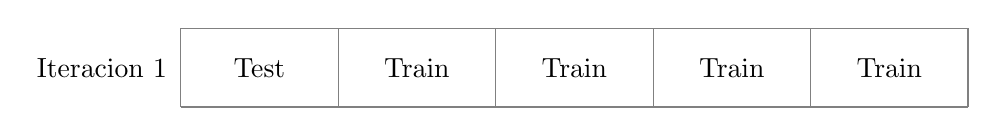
\begin{tikzpicture}
    \draw[xstep=2cm,ystep=1,color=gray] (0, 0) grid (10, 1);
    \node at (-1,0.5) {Iteracion 1};
    \node at (1,0.5) {Test};
    \node at (3,0.5) {Train};
    \node at (5,0.5) {Train};
    \node at (7,0.5) {Train};
    \node at (9,0.5) {Train};
    \end{tikzpicture}
    
    \begin{tikzpicture}
    \node at (1,0.5) {};
    \end{tikzpicture}
    
    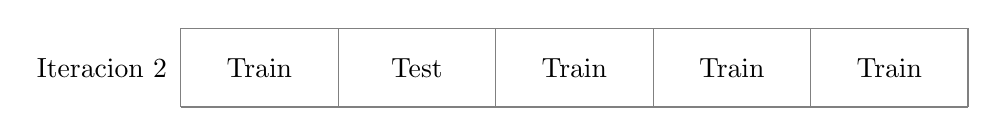
\begin{tikzpicture}
    \draw[xstep=2cm,ystep=1,color=gray] (0, 0) grid (10, 1);
    \node at (-1,0.5) {Iteracion 2};
    \node at (1,0.5) {Train};
    \node at (3,0.5) {Test};
    \node at (5,0.5) {Train};
    \node at (7,0.5) {Train};
    \node at (9,0.5) {Train};
    \end{tikzpicture}
    
    \begin{tikzpicture}
    \node at (1,0.5) {};
    \end{tikzpicture}
    
    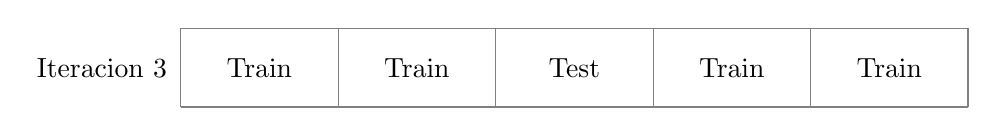
\begin{tikzpicture}
    \draw[xstep=2cm,ystep=1,color=gray] (0, 0) grid (10, 1);
    \node at (-1,0.5) {Iteracion 3};
    \node at (1,0.5) {Train};
    \node at (3,0.5) {Train};
    \node at (5,0.5) {Test};
    \node at (7,0.5) {Train};
    \node at (9,0.5) {Train};
    \end{tikzpicture}
    
    \begin{tikzpicture}
    \node at (1,0.5) {};
    \end{tikzpicture}
    
    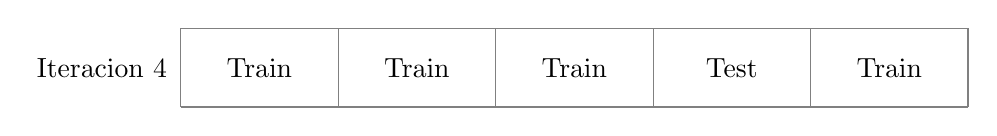
\begin{tikzpicture}
    \draw[xstep=2cm,ystep=1,color=gray] (0, 0) grid (10, 1);
    \node at (-1,0.5) {Iteracion 4};
    \node at (1,0.5) {Train};
    \node at (3,0.5) {Train};
    \node at (5,0.5) {Train};
    \node at (7,0.5) {Test};
    \node at (9,0.5) {Train};
    \end{tikzpicture}
    
    \begin{tikzpicture}
    \node at (1,0.5) {};
    \end{tikzpicture}
    
    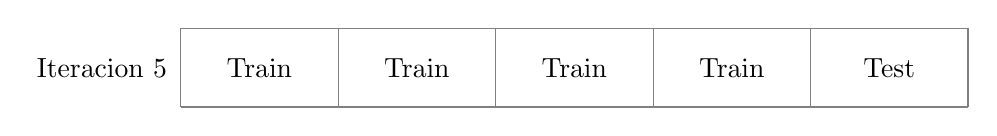
\begin{tikzpicture}
    \draw[xstep=2cm,ystep=1,color=gray] (0, 0) grid (10, 1);
    \node at (-1,0.5) {Iteracion 5};
    \node at (1,0.5) {Train};
    \node at (3,0.5) {Train};
    \node at (5,0.5) {Train};
    \node at (7,0.5) {Train};
    \node at (9,0.5) {Test};
    \end{tikzpicture}
\end{center}

Para poder comparar la calidad de los conjuntos de datos generados por los algoritmos de esta biblioteca, se ha entrenado un clasificador \textit{C4.5} \cite{c4.5} y una \textit{SVM} \cite{svm}—. Ambos clasificadores son los implementados en la librería \textit{WEKA} \cite{weka} \cite{wekaweb}. Dichos clasificadores han sido entrenados para cada una de las cinco particiones de \textit{train} comentadas anteriormente y probados contra la correspondiente partición de \textit{test}. Este proceso se ha hecho para los conjuntos de datos originales y para los conjuntos de datos reducidos por cada algoritmo. Para poder comparar los resultados se han usado las 3 métricas descritas a continuación.

\subsection{Porcentaje de acierto.} \label{subsec:porcentaje}

Es la métrica más usada en este tipo de problems y, probablemente, la más fácil de calcular y obtener. Este tipo de algoritmos pretende predecir un comportamiento y que mejor manera de medir como de bueno es el algoritmo que calculando como de buenos es prediciendo nuevas instancias. Para obtener esta métrica solo debemos predecir las clases del conjunto de \textit{test}, compararlas con las etiquetas reales de dicho conjunto y calcular que porcentaje son correctas. A mayor porcentaje, mejor es el algoritmo, ya que consigue predecir un mayor número de instancias.

\subsection{AUC.} \label{subsec:auc}

Acrónimo de \textit{Area Under Curve}, o \textit{Area Bajo la Curva}. En este proyecto se ha usado la curva \textit{ROC} —acrónimo de \textit{Receiver Operating Characteristic}, \textit{Característica Operativa del Receptor} es español— \cite{roc}. La curva ROC se obtiene dibujando el ratio de verdaderos positivos —\textit{True Positive Rate, TPR}— frente al ratio de falsos positivos —\textit{False Positive Rate, FPR}— para diferentes valores de los parámetros empleados en el algoritmo. El ratio de verdaderos positivos se puede calcular aplicando la siguiente fórmula:
\begin{equation}
	\label{eq:tpr}
	TPR = TP / (TP + FN)
\end{equation}
donde \textit{TP} representa los \textit{True Positives} —instancias positivas que se han clasificado correctamente como positivas— y \textit{FN} representa los \textit{False Negatives} —instancias positivas que se han clasificado incorrectamente como negativas—. El ratio de falsos positivos se puede calcular aplicando la siguiente fórmula:
\begin{equation}
	FPR = FN / (FP + TN)
\end{equation}
donde \textit{FN} representa los \textit{False Negatives} —instancias positivas que se han clasificado incorrectamente como negativas—, \textit{FP} representa los \textit{False Positives} —instancias negativas que se han clasificado incorrectamente como positivas— y \textit{TN} representa los \textit{True Negatives} —instancias negativas que se han clasificado correctamente como negativas—. \\

La gráfica de la curva ROC tiene la siguiente forma \footnote{Imagen creada por mí usando \textit{Python} \cite{pythonweb} y \textit{scikit-learn.} \cite{scikit-learn}}:

\begin{figure}[H]
	\includegraphics[width=\linewidth]{./imagenes/7_roc.png}
	\caption{Ejemplo curva ROC.}
	\label{img:roc}
\end{figure}

Para ver si un clasificador es bueno podemos calcular el área bajo la curva ROC. A mayor valor de área, mejor es el clasificador. En la imagen \ref{img:roc} podemos ver una línea discontinua. Dicha línea representa un área de \textit{0.5}. En dicha imagen también podemos ver que el área calculada es de \textit{0.77}, un valor bastante aceptable.

\subsection{Media geométrica.} \label{subsec:gm}

La media geométrica \cite{gm} se define como:

\begin{equation}
	g = \sqrt{a^+ \cdot a^-}
\end{equation}

donde a$^+$ denota la precisión en las instancias positivas —esto es \textit{TPR}— y a$^-$ denota la precisión en las instancias positivas —esto es \textit{TNR}—. \textit{TPR} calcula como hemos visto en la ecuación \ref{eq:tpr} y \textit{TNR} se calcula de la siguiente forma:

\begin{equation}
	TNR = \frac{TP}{TP + FN}
\end{equation}

Esta métrica une dos objetivos; busca maximizar la precisión a la vez que equilibrar el tamaño de ambas clases.

\section{Resultados numéricos.} \label{sec:resultados_numericos}

A continuación se muestran varias tablas donde iremos analizando los resultados obtenidos por los distintos algoritmos. Como se ha comentado en la sección \ref{sec:clasificacion} se ha usado \textit{k-fold} y la cantidad de datos recogida es abrumadora. Es por ello que, a continuación, se muestran las tablas con los valores medios de las cinco ejecuciones. Dichas tablas tienen un formato bastante colorido, ya que se ha aplicado un coloreado basado en \textit{mapas de calor}. Esta técnica colorea las celdas con un color más cálido —en este caso colores rojizos— cuanto mejor es el valor representado por dicha celda y un color más frío —en este caso colores azules— cuanto peor es el valor representado por dicha celda. En las tablas \ref{tab:tamanio_reducido}, \ref{tab:porcentaje_reducido} y \ref{tab:ir} se ha aplicado por filas, pudiendo comparar así el comportamiento de cada algoritmo. En las tablas \ref{tab:metricas_pt1}, \ref{tab:metricas_pt2}, \ref{tab:metricas_pt3} y \ref{tab:metricas_pt4} se ha aplicado por columnas, permitiendo comparar los algoritmos y ver el mejor valor de cada métrica. En el apéndice \ref{ch:apendice} se encuentran las tablas con toda la información recogida, para que se pueda verificar que las tablas presentadas en esta sección son reales. \\

Todas las ejecuciones han sido realizadas con los valores por defecto de los parámetros. Dichos valores los podemos ver en la sección \ref{sec:implementacion_algoritmos} o en la página web que contiene la documentación del proyecto, \href{https://nestorrv.github.io}{https://nestorrv.github.io}. \\

Para comparar como de efectivo es el proceso de reducción se ha comparado el tamaño del conjunto de datos antes y después de la aplicación de los algoritmos. Esta comparación la podemos ver en la tabla \ref{tab:tamanio_reducido}. Por lo general, el algoritmo que mejor se comporta es \textit{IPADE-ID} \cite{ipade}, junto con \textit{CPM} \cite{cpm}. En la tabla \ref{tab:porcentaje_reducido} podemos ver los porcentajes de reducción para los distintos algoritmos. Si nos fijamos en los valores medios, podemos ver que se obtiene un alto porcentaje de reducción, en torno a la mitad del tamaño original. \\

En la tabla \ref{tab:ir} podemos ver como se comporta el \textit{Imbalanced Ratio} tras aplicar los distintos algoritmos. En este caso, el algoritmo que mejor se comporta —por lo general— es \textit{IHTS} \cite{ihts} junto con \textit{ClusterOSS} \cite{clusteross}. Si nos fijamos en los valores medios, podemos ver que se obtiene un \textit{Imbalanced Ratio} bastante menor que en el conjunto de datos original, lo cual nos indica que se ha conseguido una mejor proporción de instancias positivas con respecto a instancias negativas. \\

En las tablas \ref{tab:metricas_pt1}, \ref{tab:metricas_pt2}, \ref{tab:metricas_pt3} y \ref{tab:metricas_pt4} podemos ver los valores medios de las métricas comentadas en la sección \ref{sec:clasificacion} para las cinco ejecuciones —obtenidas al aplicar \textit{k-fold}— de los conjuntos de datos antes y después de ser reducidos por los algoritmos. Como podemos ver, los valores medios obtenidos tras aplicar los algoritmos es bastante similar a la media de los conjuntos de datos original —los cuales podemos ver en la fila identificada por \textit{original}—. En todos los casos, hay un algoritmo que mejora los valores del conjunto original. \\

Tal y como hemos visto en esta sección, realizar un proceso de \textit{undersampling} aporta ventajas, pero tiene un inconveniente, y es que no es un proceso gratis. Este proceso lleva asociado un tiempo de ejecución. En la tabla \ref{tab:tiempos} podemos ver los tiempos de ejecución de cada algoritmo en cada conjunto de datos. El formato de dicha tabla es: \textit{minutos:segundos:milisegundos}. Como podemos ver, la mayoría de los algoritmos son bastante rápidos, excepto \textit{EUS} \cite{eus} e \textit{IPADE-ID}, ya que al ser algoritmos evolutivos necesitan más tiempo de ejecución. 

\hvFloat[
 floatPos=!htb,
 capWidth=h,
 capPos=r,
 capAngle=90,
 objectAngle=90,
 capVPos=c,
 objectPos=c]{table}{\scalebox{0.7}{\begin{tabular}{l|c|ccccccccccccccc|c}
\textbf{Dataset} & \textbf{Tamaño Original} & \textbf{BC} & \textbf{ClusterOSS} & \textbf{CNN} & \textbf{CPM} & \textbf{EE} & \textbf{ENN} & \textbf{EUS} & \textbf{IHTS} & \textbf{IPADE} & \textbf{NCL} & \textbf{NM} & \textbf{OSS} & \textbf{RU} & \textbf{SBC} & \textbf{TL} & \textbf{Media} \\
\midrule
\textbf{ecoli-0\_vs\_1} & 220   & \cellcolor[rgb]{ .988,  .988,  1}154 & \cellcolor[rgb]{ .976,  .608,  .616}64 & \cellcolor[rgb]{ .973,  .412,  .42}17 & \cellcolor[rgb]{ .973,  .416,  .424}18 & \cellcolor[rgb]{ .988,  .988,  1}154 & \cellcolor[rgb]{ .353,  .541,  .776}220 & \cellcolor[rgb]{ .988,  .988,  1}154 & \cellcolor[rgb]{ .98,  .784,  .796}106 & \cellcolor[rgb]{ .973,  .42,  .427}19 & \cellcolor[rgb]{ .451,  .612,  .812}210 & \cellcolor[rgb]{ .988,  .988,  1}154 & \cellcolor[rgb]{ .984,  .875,  .882}127 & \cellcolor[rgb]{ .988,  .988,  1}154 & \cellcolor[rgb]{ .443,  .604,  .808}211 & \cellcolor[rgb]{ .451,  .612,  .812}210 & 131.46667 \\
\textbf{ecoli1} & 336   & \cellcolor[rgb]{ .988,  .988,  1}154 & \cellcolor[rgb]{ .973,  .502,  .514}56 & \cellcolor[rgb]{ .976,  .624,  .631}80 & \cellcolor[rgb]{ .976,  .647,  .655}85 & \cellcolor[rgb]{ .988,  .988,  1}154 & \cellcolor[rgb]{ .353,  .541,  .776}321 & \cellcolor[rgb]{ .988,  .988,  1}154 & \cellcolor[rgb]{ .976,  .663,  .671}88 & \cellcolor[rgb]{ .973,  .412,  .42}37 & \cellcolor[rgb]{ .439,  .604,  .808}299 & \cellcolor[rgb]{ .988,  .988,  1}154 & \cellcolor[rgb]{ .718,  .796,  .906}226 & \cellcolor[rgb]{ .988,  .988,  1}154 & \cellcolor[rgb]{ .471,  .624,  .82}291 & \cellcolor[rgb]{ .451,  .612,  .812}296 & 169.93333 \\
\textbf{ecoli2} & 336   & \cellcolor[rgb]{ .988,  .988,  1}104 & \cellcolor[rgb]{ .973,  .482,  .49}34 & \cellcolor[rgb]{ .98,  .722,  .729}67 & \cellcolor[rgb]{ .976,  .69,  .702}63 & \cellcolor[rgb]{ .988,  .988,  1}104 & \cellcolor[rgb]{ .353,  .541,  .776}329 & \cellcolor[rgb]{ .988,  .988,  1}104 & \cellcolor[rgb]{ .976,  .69,  .702}63 & \cellcolor[rgb]{ .973,  .412,  .42}24 & \cellcolor[rgb]{ .388,  .569,  .792}317 & \cellcolor[rgb]{ .988,  .988,  1}104 & \cellcolor[rgb]{ .49,  .639,  .827}281 & \cellcolor[rgb]{ .988,  .988,  1}104 & \cellcolor[rgb]{ .412,  .584,  .8}309 & \cellcolor[rgb]{ .404,  .576,  .796}312 & 154.6 \\
\textbf{ecoli3} & 336   & \cellcolor[rgb]{ .988,  .988,  1}70 & \cellcolor[rgb]{ .973,  .549,  .561}42 & \cellcolor[rgb]{ .984,  .894,  .906}64 & \cellcolor[rgb]{ .976,  .675,  .686}50 & \cellcolor[rgb]{ .988,  .988,  1}70 & \cellcolor[rgb]{ .353,  .541,  .776}324 & \cellcolor[rgb]{ .988,  .988,  1}70 & \cellcolor[rgb]{ .976,  .627,  .639}47 & \cellcolor[rgb]{ .973,  .412,  .42}33 & \cellcolor[rgb]{ .38,  .561,  .788}314 & \cellcolor[rgb]{ .988,  .988,  1}70 & \cellcolor[rgb]{ .541,  .675,  .843}250 & \cellcolor[rgb]{ .988,  .988,  1}70 & \cellcolor[rgb]{ .408,  .58,  .796}303 & \cellcolor[rgb]{ .388,  .569,  .792}310 & 139.13333 \\
\textbf{glass-0-1-2-3\_vs\_4-5-6} & 214   & \cellcolor[rgb]{ .988,  .988,  1}102 & \cellcolor[rgb]{ .973,  .424,  .435}30 & \cellcolor[rgb]{ .973,  .431,  .443}31 & \cellcolor[rgb]{ .973,  .412,  .42}28 & \cellcolor[rgb]{ .988,  .988,  1}102 & \cellcolor[rgb]{ .353,  .541,  .776}206 & \cellcolor[rgb]{ .988,  .988,  1}102 & \cellcolor[rgb]{ .976,  .627,  .639}56 & \cellcolor[rgb]{ .973,  .431,  .443}31 & \cellcolor[rgb]{ .416,  .584,  .8}196 & \cellcolor[rgb]{ .988,  .988,  1}102 & \cellcolor[rgb]{ .416,  .584,  .8}196 & \cellcolor[rgb]{ .988,  .988,  1}102 & \cellcolor[rgb]{ .38,  .561,  .788}202 & \cellcolor[rgb]{ .38,  .561,  .788}202 & 112.53333 \\
\textbf{glass0} & 214   & \cellcolor[rgb]{ .988,  .988,  1}140 & \cellcolor[rgb]{ .973,  .427,  .435}41 & \cellcolor[rgb]{ .976,  .635,  .647}78 & \cellcolor[rgb]{ .976,  .604,  .612}72 & \cellcolor[rgb]{ .988,  .988,  1}140 & \cellcolor[rgb]{ .353,  .541,  .776}183 & \cellcolor[rgb]{ .988,  .988,  1}140 & \cellcolor[rgb]{ .98,  .749,  .761}98 & \cellcolor[rgb]{ .973,  .412,  .42}38 & \cellcolor[rgb]{ .533,  .667,  .839}171 & \cellcolor[rgb]{ .988,  .988,  1}140 & \cellcolor[rgb]{ .984,  .953,  .965}134 & \cellcolor[rgb]{ .988,  .988,  1}140 & \cellcolor[rgb]{ .443,  .604,  .808}177 & \cellcolor[rgb]{ .545,  .678,  .847}170 & 124.13333 \\
\textbf{glass1} & 214   & \cellcolor[rgb]{ .988,  .988,  1}152 & \cellcolor[rgb]{ .973,  .412,  .42}34 & \cellcolor[rgb]{ .976,  .671,  .678}87 & \cellcolor[rgb]{ .976,  .639,  .647}81 & \cellcolor[rgb]{ .988,  .988,  1}152 & \cellcolor[rgb]{ .353,  .541,  .776}192 & \cellcolor[rgb]{ .988,  .988,  1}152 & \cellcolor[rgb]{ .98,  .804,  .816}115 & \cellcolor[rgb]{ .973,  .439,  .447}40 & \cellcolor[rgb]{ .69,  .776,  .894}171 & \cellcolor[rgb]{ .988,  .988,  1}152 & \cellcolor[rgb]{ .816,  .867,  .941}163 & \cellcolor[rgb]{ .988,  .988,  1}152 & \cellcolor[rgb]{ .467,  .62,  .816}185 & \cellcolor[rgb]{ .671,  .765,  .89}172 & 133.33333 \\
\textbf{glass6} & 214   & \cellcolor[rgb]{ .988,  .988,  1}58 & \cellcolor[rgb]{ .976,  .663,  .671}36 & \cellcolor[rgb]{ .973,  .412,  .42}19 & \cellcolor[rgb]{ .973,  .455,  .463}22 & \cellcolor[rgb]{ .988,  .988,  1}58 & \cellcolor[rgb]{ .353,  .541,  .776}213 & \cellcolor[rgb]{ .988,  .988,  1}58 & \cellcolor[rgb]{ .976,  .631,  .639}34 & \cellcolor[rgb]{ .973,  .514,  .522}26 & \cellcolor[rgb]{ .416,  .588,  .8}198 & \cellcolor[rgb]{ .988,  .988,  1}58 & \cellcolor[rgb]{ .871,  .906,  .961}87 & \cellcolor[rgb]{ .988,  .988,  1}58 & \cellcolor[rgb]{ .4,  .576,  .796}202 & \cellcolor[rgb]{ .4,  .576,  .796}202 & 88.6 \\
\textbf{haberman} & 306   & \cellcolor[rgb]{ .988,  .988,  1}162 & \cellcolor[rgb]{ .973,  .49,  .498}55 & \cellcolor[rgb]{ .984,  .984,  1}163 & \cellcolor[rgb]{ .984,  .918,  .929}147 & \cellcolor[rgb]{ .988,  .988,  1}162 & \cellcolor[rgb]{ .353,  .541,  .776}273 & \cellcolor[rgb]{ .984,  .984,  1}163 & \cellcolor[rgb]{ .976,  .616,  .624}82 & \cellcolor[rgb]{ .973,  .412,  .42}38 & \cellcolor[rgb]{ .573,  .698,  .855}235 & \cellcolor[rgb]{ .988,  .988,  1}162 & \cellcolor[rgb]{ .769,  .831,  .922}201 & \cellcolor[rgb]{ .988,  .988,  1}162 & \cellcolor[rgb]{ .722,  .8,  .906}209 & \cellcolor[rgb]{ .706,  .788,  .902}212 & 161.73333 \\
\textbf{iris0} & 150   & \cellcolor[rgb]{ .988,  .988,  1}100 & \cellcolor[rgb]{ .973,  .475,  .482}13 & \cellcolor[rgb]{ .973,  .412,  .42}2 & \cellcolor[rgb]{ .973,  .412,  .42}2 & \cellcolor[rgb]{ .988,  .988,  1}100 & \cellcolor[rgb]{ .353,  .541,  .776}150 & \cellcolor[rgb]{ .988,  .988,  1}100 & \cellcolor[rgb]{ .98,  .8,  .808}68 & \cellcolor[rgb]{ .973,  .475,  .482}13 & \cellcolor[rgb]{ .353,  .541,  .776}150 & \cellcolor[rgb]{ .988,  .988,  1}100 & \cellcolor[rgb]{ .976,  .686,  .694}49 & \cellcolor[rgb]{ .988,  .988,  1}100 & \cellcolor[rgb]{ .38,  .561,  .788}148 & \cellcolor[rgb]{ .404,  .58,  .796}146 & 82.73333 \\
\textbf{new-thyroid1} & 215   & \cellcolor[rgb]{ .988,  .988,  1}70 & \cellcolor[rgb]{ .98,  .702,  .714}41 & \cellcolor[rgb]{ .973,  .412,  .42}11 & \cellcolor[rgb]{ .973,  .427,  .439}13 & \cellcolor[rgb]{ .988,  .988,  1}70 & \cellcolor[rgb]{ .353,  .541,  .776}213 & \cellcolor[rgb]{ .988,  .988,  1}70 & \cellcolor[rgb]{ .984,  .969,  .976}68 & \cellcolor[rgb]{ .973,  .537,  .545}24 & \cellcolor[rgb]{ .404,  .576,  .796}202 & \cellcolor[rgb]{ .988,  .988,  1}70 & \cellcolor[rgb]{ .984,  .898,  .91}61 & \cellcolor[rgb]{ .988,  .988,  1}70 & \cellcolor[rgb]{ .376,  .557,  .784}208 & \cellcolor[rgb]{ .392,  .569,  .792}205 & 93.06667 \\
\textbf{new-thyroid2} & 215   & \cellcolor[rgb]{ .988,  .988,  1}70 & \cellcolor[rgb]{ .976,  .631,  .639}36 & \cellcolor[rgb]{ .973,  .412,  .42}15 & \cellcolor[rgb]{ .973,  .42,  .427}16 & \cellcolor[rgb]{ .988,  .988,  1}70 & \cellcolor[rgb]{ .353,  .541,  .776}213 & \cellcolor[rgb]{ .988,  .988,  1}70 & \cellcolor[rgb]{ .976,  .671,  .682}40 & \cellcolor[rgb]{ .973,  .494,  .502}23 & \cellcolor[rgb]{ .4,  .573,  .792}203 & \cellcolor[rgb]{ .988,  .988,  1}70 & \cellcolor[rgb]{ .886,  .918,  .965}93 & \cellcolor[rgb]{ .988,  .988,  1}70 & \cellcolor[rgb]{ .384,  .565,  .788}206 & \cellcolor[rgb]{ .392,  .569,  .792}205 & 93.33333 \\
\textbf{page-blocks0} & 5472  & \cellcolor[rgb]{ .988,  .988,  1}1118 & \cellcolor[rgb]{ .976,  .624,  .635}502 & \cellcolor[rgb]{ .976,  .631,  .643}514 & \cellcolor[rgb]{ .976,  .631,  .643}514 & \cellcolor[rgb]{ .988,  .988,  1}1118 & \cellcolor[rgb]{ .353,  .541,  .776}5410 & \cellcolor[rgb]{ .984,  .984,  .996}1117 & \cellcolor[rgb]{ .98,  .722,  .729}665 & \cellcolor[rgb]{ .973,  .412,  .42}135 & \cellcolor[rgb]{ .376,  .561,  .788}5255 & \cellcolor[rgb]{ .988,  .988,  1}1118 & \cellcolor[rgb]{ .475,  .627,  .82}4598 & \cellcolor[rgb]{ .988,  .988,  1}1118 & \cellcolor[rgb]{ .667,  .761,  .886}3312 & \cellcolor[rgb]{ .388,  .565,  .788}5186 & 2112 \\
\textbf{pima} & 768   & \cellcolor[rgb]{ .988,  .988,  1}536 & \cellcolor[rgb]{ .973,  .537,  .545}161 & \cellcolor[rgb]{ .98,  .796,  .808}377 & \cellcolor[rgb]{ .98,  .792,  .804}374 & \cellcolor[rgb]{ .988,  .988,  1}536 & \cellcolor[rgb]{ .353,  .541,  .776}678 & \cellcolor[rgb]{ .984,  .984,  .996}535 & \cellcolor[rgb]{ .976,  .686,  .698}287 & \cellcolor[rgb]{ .973,  .412,  .42}55 & \cellcolor[rgb]{ .792,  .851,  .933}580 & \cellcolor[rgb]{ .988,  .988,  1}536 & \cellcolor[rgb]{ .98,  .984,  1}538 & \cellcolor[rgb]{ .988,  .988,  1}536 & \cellcolor[rgb]{ .988,  .988,  1}536 & \cellcolor[rgb]{ .89,  .922,  .969}558 & 454.86667 \\
\textbf{segment0} & 2308  & \cellcolor[rgb]{ .988,  .988,  1}658 & \cellcolor[rgb]{ .976,  .643,  .651}287 & \cellcolor[rgb]{ .973,  .439,  .447}69 & \cellcolor[rgb]{ .973,  .435,  .443}65 & \cellcolor[rgb]{ .988,  .988,  1}658 & \cellcolor[rgb]{ .353,  .541,  .776}2290 & \cellcolor[rgb]{ .984,  .98,  .992}652 & \cellcolor[rgb]{ .965,  .973,  .992}725 & \cellcolor[rgb]{ .973,  .412,  .42}38 & \cellcolor[rgb]{ .361,  .545,  .78}2277 & \cellcolor[rgb]{ .988,  .988,  1}658 & \cellcolor[rgb]{ .529,  .667,  .839}1841 & \cellcolor[rgb]{ .988,  .988,  1}658 & \cellcolor[rgb]{ .533,  .671,  .843}1830 & \cellcolor[rgb]{ .4,  .576,  .796}2172 & 991.86667 \\
\textbf{vehicle0} & 846   & \cellcolor[rgb]{ .988,  .988,  1}398 & \cellcolor[rgb]{ .973,  .541,  .553}148 & \cellcolor[rgb]{ .973,  .518,  .525}133 & \cellcolor[rgb]{ .973,  .553,  .561}154 & \cellcolor[rgb]{ .988,  .988,  1}398 & \cellcolor[rgb]{ .353,  .541,  .776}829 & \cellcolor[rgb]{ .988,  .988,  1}399 & \cellcolor[rgb]{ .984,  .894,  .902}345 & \cellcolor[rgb]{ .973,  .412,  .42}73 & \cellcolor[rgb]{ .416,  .588,  .8}787 & \cellcolor[rgb]{ .988,  .988,  1}398 & \cellcolor[rgb]{ .51,  .651,  .831}724 & \cellcolor[rgb]{ .988,  .988,  1}398 & \cellcolor[rgb]{ .561,  .686,  .851}690 & \cellcolor[rgb]{ .494,  .643,  .827}734 & 440.53333 \\
\textbf{vehicle1} & 846   & \cellcolor[rgb]{ .988,  .988,  1}434 & \cellcolor[rgb]{ .973,  .467,  .475}187 & \cellcolor[rgb]{ .984,  .871,  .882}380 & \cellcolor[rgb]{ .984,  .886,  .894}386 & \cellcolor[rgb]{ .988,  .988,  1}434 & \cellcolor[rgb]{ .353,  .541,  .776}756 & \cellcolor[rgb]{ .984,  .961,  .973}422 & \cellcolor[rgb]{ .976,  .69,  .698}293 & \cellcolor[rgb]{ .973,  .412,  .42}161 & \cellcolor[rgb]{ .541,  .675,  .843}661 & \cellcolor[rgb]{ .988,  .988,  1}434 & \cellcolor[rgb]{ .639,  .741,  .878}612 & \cellcolor[rgb]{ .988,  .988,  1}434 & \cellcolor[rgb]{ .733,  .808,  .91}565 & \cellcolor[rgb]{ .627,  .733,  .875}618 & 451.8 \\
\textbf{vehicle2} & 846   & \cellcolor[rgb]{ .988,  .988,  1}436 & \cellcolor[rgb]{ .976,  .573,  .58}161 & \cellcolor[rgb]{ .973,  .537,  .545}138 & \cellcolor[rgb]{ .973,  .545,  .553}143 & \cellcolor[rgb]{ .988,  .988,  1}436 & \cellcolor[rgb]{ .353,  .541,  .776}816 & \cellcolor[rgb]{ .984,  .98,  .992}433 & \cellcolor[rgb]{ .984,  .863,  .871}353 & \cellcolor[rgb]{ .973,  .412,  .42}53 & \cellcolor[rgb]{ .412,  .58,  .796}783 & \cellcolor[rgb]{ .988,  .988,  1}436 & \cellcolor[rgb]{ .502,  .647,  .831}729 & \cellcolor[rgb]{ .988,  .988,  1}436 & \cellcolor[rgb]{ .69,  .78,  .898}616 & \cellcolor[rgb]{ .49,  .635,  .824}736 & 447 \\
\textbf{vehicle3} & 846   & \cellcolor[rgb]{ .988,  .988,  1}424 & \cellcolor[rgb]{ .973,  .412,  .42}127 & \cellcolor[rgb]{ .984,  .855,  .867}356 & \cellcolor[rgb]{ .984,  .882,  .894}370 & \cellcolor[rgb]{ .988,  .988,  1}424 & \cellcolor[rgb]{ .353,  .541,  .776}774 & \cellcolor[rgb]{ .984,  .973,  .984}417 & \cellcolor[rgb]{ .929,  .945,  .98}458 & \cellcolor[rgb]{ .973,  .416,  .424}131 & \cellcolor[rgb]{ .537,  .671,  .843}674 & \cellcolor[rgb]{ .988,  .988,  1}424 & \cellcolor[rgb]{ .651,  .753,  .882}610 & \cellcolor[rgb]{ .988,  .988,  1}424 & \cellcolor[rgb]{ .745,  .82,  .918}558 & \cellcolor[rgb]{ .627,  .733,  .875}624 & 453 \\
\textbf{wisconsin} & 683   & \cellcolor[rgb]{ .988,  .988,  1}478 & \cellcolor[rgb]{ .973,  .412,  .42}28 & \cellcolor[rgb]{ .973,  .471,  .478}74 & \cellcolor[rgb]{ .973,  .467,  .475}73 & \cellcolor[rgb]{ .988,  .988,  1}478 & \cellcolor[rgb]{ .384,  .565,  .788}672 & \cellcolor[rgb]{ .988,  .988,  1}478 & \cellcolor[rgb]{ .984,  .914,  .925}421 & \cellcolor[rgb]{ .973,  .439,  .447}52 & \cellcolor[rgb]{ .416,  .584,  .8}662 & \cellcolor[rgb]{ .988,  .988,  1}478 & \cellcolor[rgb]{ .98,  .761,  .773}303 & \cellcolor[rgb]{ .988,  .988,  1}478 & \cellcolor[rgb]{ .353,  .541,  .776}681 & \cellcolor[rgb]{ .412,  .584,  .8}663 & 401.26667 \\
\textbf{yeast1} & 1484  & \cellcolor[rgb]{ .988,  .988,  1}858 & \cellcolor[rgb]{ .973,  .525,  .537}294 & \cellcolor[rgb]{ .984,  .843,  .855}681 & \cellcolor[rgb]{ .984,  .855,  .867}696 & \cellcolor[rgb]{ .988,  .988,  1}858 & \cellcolor[rgb]{ .514,  .655,  .835}1325 & \cellcolor[rgb]{ .988,  .988,  1}859 & \cellcolor[rgb]{ .98,  .702,  .71}508 & \cellcolor[rgb]{ .973,  .412,  .42}150 & \cellcolor[rgb]{ .698,  .784,  .898}1146 & \cellcolor[rgb]{ .988,  .988,  1}858 & \cellcolor[rgb]{ .733,  .808,  .91}1111 & \cellcolor[rgb]{ .988,  .988,  1}858 & \cellcolor[rgb]{ .353,  .541,  .776}1481 & \cellcolor[rgb]{ .729,  .808,  .91}1114 & 853.13333 \\
\textbf{yeast3} & 1484  & \cellcolor[rgb]{ .988,  .988,  1}326 & \cellcolor[rgb]{ .976,  .557,  .565}151 & \cellcolor[rgb]{ .98,  .788,  .796}245 & \cellcolor[rgb]{ .98,  .769,  .78}238 & \cellcolor[rgb]{ .988,  .988,  1}326 & \cellcolor[rgb]{ .353,  .541,  .776}1451 & \cellcolor[rgb]{ .988,  .988,  1}326 & \cellcolor[rgb]{ .976,  .624,  .635}179 & \cellcolor[rgb]{ .973,  .412,  .42}92 & \cellcolor[rgb]{ .388,  .565,  .788}1395 & \cellcolor[rgb]{ .988,  .988,  1}326 & \cellcolor[rgb]{ .404,  .58,  .796}1362 & \cellcolor[rgb]{ .988,  .988,  1}326 & \cellcolor[rgb]{ .549,  .678,  .847}1109 & \cellcolor[rgb]{ .404,  .58,  .796}1362 & 614.26667 \\
\end{tabular}}}{Tamaño de los conjuntos de datos reducidos.}{tab:tamanio_reducido}

\hvFloat[
 floatPos=!htb,
 capWidth=h,
 capPos=r,
 capAngle=90,
 objectAngle=90,
 capVPos=c,
 objectPos=c]{table}{\scalebox{0.7}{\begin{tabular}{l|ccccccccccccccc|c}
\textbf{Dataset} & \textbf{BC} & \textbf{ClusterOSS} & \textbf{CNN} & \textbf{CPM} & \textbf{EE} & \textbf{ENN} & \textbf{EUS} & \textbf{IHTS} & \textbf{IPADE} & \textbf{NCL} & \textbf{NM} & \textbf{OSS} & \textbf{RU} & \textbf{SBC} & \textbf{TL} & \textbf{Media} \\
\midrule
\textbf{ecoli-0\_vs\_1} & \cellcolor[rgb]{ .988,  .988,  1}30 & \cellcolor[rgb]{ .98,  .612,  .62}70.91 & \cellcolor[rgb]{ .973,  .412,  .42}92.27 & \cellcolor[rgb]{ .976,  .42,  .427}91.82 & \cellcolor[rgb]{ .988,  .988,  1}30 & \cellcolor[rgb]{ .353,  .541,  .776}0 & \cellcolor[rgb]{ .988,  .988,  1}30 & \cellcolor[rgb]{ .984,  .788,  .8}51.82 & \cellcolor[rgb]{ .976,  .424,  .431}91.36 & \cellcolor[rgb]{ .447,  .608,  .808}4.55 & \cellcolor[rgb]{ .988,  .988,  1}30 & \cellcolor[rgb]{ .988,  .878,  .886}42.27 & \cellcolor[rgb]{ .988,  .988,  1}30 & \cellcolor[rgb]{ .439,  .6,  .804}4.09 & \cellcolor[rgb]{ .447,  .608,  .808}4.55 & 40.24 \\
\textbf{ecoli1} & \cellcolor[rgb]{ .988,  .988,  1}54.17 & \cellcolor[rgb]{ .976,  .506,  .518}83.33 & \cellcolor[rgb]{ .98,  .627,  .635}76.19 & \cellcolor[rgb]{ .98,  .651,  .659}74.7 & \cellcolor[rgb]{ .988,  .988,  1}54.17 & \cellcolor[rgb]{ .353,  .541,  .776}4.46 & \cellcolor[rgb]{ .988,  .988,  1}54.17 & \cellcolor[rgb]{ .98,  .667,  .675}73.81 & \cellcolor[rgb]{ .973,  .412,  .42}88.99 & \cellcolor[rgb]{ .435,  .6,  .804}11.01 & \cellcolor[rgb]{ .988,  .988,  1}54.17 & \cellcolor[rgb]{ .714,  .792,  .902}32.74 & \cellcolor[rgb]{ .988,  .988,  1}54.17 & \cellcolor[rgb]{ .467,  .62,  .816}13.39 & \cellcolor[rgb]{ .447,  .608,  .808}11.9 & 49.42 \\
\textbf{ecoli2} & \cellcolor[rgb]{ .988,  .988,  1}69.05 & \cellcolor[rgb]{ .976,  .486,  .494}89.88 & \cellcolor[rgb]{ .984,  .725,  .733}80.06 & \cellcolor[rgb]{ .98,  .694,  .706}81.25 & \cellcolor[rgb]{ .988,  .988,  1}69.05 & \cellcolor[rgb]{ .353,  .541,  .776}2.08 & \cellcolor[rgb]{ .988,  .988,  1}69.05 & \cellcolor[rgb]{ .98,  .694,  .706}81.25 & \cellcolor[rgb]{ .973,  .412,  .42}92.86 & \cellcolor[rgb]{ .384,  .565,  .788}5.65 & \cellcolor[rgb]{ .988,  .988,  1}69.05 & \cellcolor[rgb]{ .486,  .635,  .824}16.37 & \cellcolor[rgb]{ .988,  .988,  1}69.05 & \cellcolor[rgb]{ .408,  .58,  .796}8.04 & \cellcolor[rgb]{ .4,  .573,  .792}7.14 & 53.99 \\
\textbf{ecoli3} & \cellcolor[rgb]{ .988,  .988,  1}79.17 & \cellcolor[rgb]{ .976,  .553,  .565}87.5 & \cellcolor[rgb]{ .988,  .898,  .91}80.95 & \cellcolor[rgb]{ .98,  .678,  .69}85.12 & \cellcolor[rgb]{ .988,  .988,  1}79.17 & \cellcolor[rgb]{ .353,  .541,  .776}3.57 & \cellcolor[rgb]{ .988,  .988,  1}79.17 & \cellcolor[rgb]{ .98,  .631,  .643}86.01 & \cellcolor[rgb]{ .973,  .412,  .42}90.18 & \cellcolor[rgb]{ .376,  .557,  .784}6.55 & \cellcolor[rgb]{ .988,  .988,  1}79.17 & \cellcolor[rgb]{ .537,  .671,  .839}25.6 & \cellcolor[rgb]{ .988,  .988,  1}79.17 & \cellcolor[rgb]{ .404,  .576,  .792}9.82 & \cellcolor[rgb]{ .384,  .565,  .788}7.74 & 58.59 \\
\textbf{glass-0-1-2-3\_vs\_4-5-6} & \cellcolor[rgb]{ .988,  .988,  1}52.34 & \cellcolor[rgb]{ .976,  .427,  .439}85.98 & \cellcolor[rgb]{ .976,  .435,  .447}85.51 & \cellcolor[rgb]{ .973,  .412,  .42}86.92 & \cellcolor[rgb]{ .988,  .988,  1}52.34 & \cellcolor[rgb]{ .353,  .541,  .776}3.74 & \cellcolor[rgb]{ .988,  .988,  1}52.34 & \cellcolor[rgb]{ .98,  .631,  .643}73.83 & \cellcolor[rgb]{ .976,  .435,  .447}85.51 & \cellcolor[rgb]{ .412,  .58,  .796}8.41 & \cellcolor[rgb]{ .988,  .988,  1}52.34 & \cellcolor[rgb]{ .412,  .58,  .796}8.41 & \cellcolor[rgb]{ .988,  .988,  1}52.34 & \cellcolor[rgb]{ .376,  .557,  .784}5.61 & \cellcolor[rgb]{ .376,  .557,  .784}5.61 & 47.41 \\
\textbf{glass0} & \cellcolor[rgb]{ .988,  .988,  1}34.58 & \cellcolor[rgb]{ .976,  .431,  .439}80.84 & \cellcolor[rgb]{ .98,  .639,  .651}63.55 & \cellcolor[rgb]{ .98,  .604,  .616}66.36 & \cellcolor[rgb]{ .988,  .988,  1}34.58 & \cellcolor[rgb]{ .353,  .541,  .776}14.49 & \cellcolor[rgb]{ .988,  .988,  1}34.58 & \cellcolor[rgb]{ .984,  .753,  .765}54.21 & \cellcolor[rgb]{ .973,  .412,  .42}82.24 & \cellcolor[rgb]{ .529,  .663,  .835}20.09 & \cellcolor[rgb]{ .988,  .988,  1}34.58 & \cellcolor[rgb]{ .988,  .957,  .969}37.38 & \cellcolor[rgb]{ .988,  .988,  1}34.58 & \cellcolor[rgb]{ .439,  .6,  .804}17.29 & \cellcolor[rgb]{ .541,  .675,  .843}20.56 & 41.99 \\
\textbf{glass1} & \cellcolor[rgb]{ .988,  .988,  1}28.97 & \cellcolor[rgb]{ .973,  .412,  .42}84.11 & \cellcolor[rgb]{ .98,  .675,  .682}59.35 & \cellcolor[rgb]{ .98,  .643,  .651}62.15 & \cellcolor[rgb]{ .988,  .988,  1}28.97 & \cellcolor[rgb]{ .353,  .541,  .776}10.28 & \cellcolor[rgb]{ .988,  .988,  1}28.97 & \cellcolor[rgb]{ .984,  .808,  .82}46.26 & \cellcolor[rgb]{ .976,  .443,  .451}81.31 & \cellcolor[rgb]{ .686,  .773,  .89}20.09 & \cellcolor[rgb]{ .988,  .988,  1}28.97 & \cellcolor[rgb]{ .812,  .863,  .937}23.83 & \cellcolor[rgb]{ .988,  .988,  1}28.97 & \cellcolor[rgb]{ .463,  .616,  .812}13.55 & \cellcolor[rgb]{ .671,  .765,  .886}19.63 & 37.69 \\
\textbf{glass6} & \cellcolor[rgb]{ .988,  .988,  1}72.9 & \cellcolor[rgb]{ .98,  .667,  .675}83.18 & \cellcolor[rgb]{ .973,  .412,  .42}91.12 & \cellcolor[rgb]{ .976,  .459,  .467}89.72 & \cellcolor[rgb]{ .988,  .988,  1}72.9 & \cellcolor[rgb]{ .353,  .541,  .776}0.47 & \cellcolor[rgb]{ .988,  .988,  1}72.9 & \cellcolor[rgb]{ .98,  .635,  .643}84.11 & \cellcolor[rgb]{ .976,  .518,  .525}87.85 & \cellcolor[rgb]{ .412,  .584,  .796}7.48 & \cellcolor[rgb]{ .988,  .988,  1}72.9 & \cellcolor[rgb]{ .867,  .902,  .957}59.35 & \cellcolor[rgb]{ .988,  .988,  1}72.9 & \cellcolor[rgb]{ .396,  .573,  .792}5.61 & \cellcolor[rgb]{ .396,  .573,  .792}5.61 & 58.6 \\
\textbf{haberman} & \cellcolor[rgb]{ .988,  .988,  1}47.06 & \cellcolor[rgb]{ .976,  .494,  .502}82.03 & \cellcolor[rgb]{ .98,  .98,  .996}46.73 & \cellcolor[rgb]{ .988,  .922,  .933}51.96 & \cellcolor[rgb]{ .988,  .988,  1}47.06 & \cellcolor[rgb]{ .353,  .541,  .776}10.78 & \cellcolor[rgb]{ .98,  .98,  .996}46.73 & \cellcolor[rgb]{ .98,  .62,  .627}73.2 & \cellcolor[rgb]{ .973,  .412,  .42}87.58 & \cellcolor[rgb]{ .569,  .694,  .851}23.2 & \cellcolor[rgb]{ .988,  .988,  1}47.06 & \cellcolor[rgb]{ .765,  .827,  .918}34.31 & \cellcolor[rgb]{ .988,  .988,  1}47.06 & \cellcolor[rgb]{ .718,  .796,  .902}31.7 & \cellcolor[rgb]{ .702,  .784,  .898}30.72 & 47.15 \\
\textbf{iris0} & \cellcolor[rgb]{ .988,  .988,  1}33.33 & \cellcolor[rgb]{ .976,  .478,  .486}91.33 & \cellcolor[rgb]{ .973,  .412,  .42}98.67 & \cellcolor[rgb]{ .973,  .412,  .42}98.67 & \cellcolor[rgb]{ .988,  .988,  1}33.33 & \cellcolor[rgb]{ .353,  .541,  .776}0 & \cellcolor[rgb]{ .988,  .988,  1}33.33 & \cellcolor[rgb]{ .984,  .8,  .812}54.67 & \cellcolor[rgb]{ .976,  .478,  .486}91.33 & \cellcolor[rgb]{ .353,  .541,  .776}0 & \cellcolor[rgb]{ .988,  .988,  1}33.33 & \cellcolor[rgb]{ .98,  .69,  .698}67.33 & \cellcolor[rgb]{ .988,  .988,  1}33.33 & \cellcolor[rgb]{ .376,  .557,  .784}1.33 & \cellcolor[rgb]{ .4,  .576,  .792}2.67 & 44.84 \\
\textbf{new-thyroid1} & \cellcolor[rgb]{ .988,  .988,  1}67.44 & \cellcolor[rgb]{ .984,  .706,  .718}80.93 & \cellcolor[rgb]{ .973,  .412,  .42}94.88 & \cellcolor[rgb]{ .976,  .431,  .443}93.95 & \cellcolor[rgb]{ .988,  .988,  1}67.44 & \cellcolor[rgb]{ .353,  .541,  .776}0.93 & \cellcolor[rgb]{ .988,  .988,  1}67.44 & \cellcolor[rgb]{ .988,  .973,  .98}68.37 & \cellcolor[rgb]{ .976,  .541,  .549}88.84 & \cellcolor[rgb]{ .4,  .573,  .792}6.05 & \cellcolor[rgb]{ .988,  .988,  1}67.44 & \cellcolor[rgb]{ .988,  .902,  .914}71.63 & \cellcolor[rgb]{ .988,  .988,  1}67.44 & \cellcolor[rgb]{ .373,  .553,  .78}3.26 & \cellcolor[rgb]{ .388,  .565,  .788}4.65 & 56.71 \\
\textbf{new-thyroid2} & \cellcolor[rgb]{ .988,  .988,  1}67.44 & \cellcolor[rgb]{ .98,  .635,  .643}83.26 & \cellcolor[rgb]{ .973,  .412,  .42}93.02 & \cellcolor[rgb]{ .976,  .424,  .431}92.56 & \cellcolor[rgb]{ .988,  .988,  1}67.44 & \cellcolor[rgb]{ .353,  .541,  .776}0.93 & \cellcolor[rgb]{ .988,  .988,  1}67.44 & \cellcolor[rgb]{ .98,  .675,  .686}81.4 & \cellcolor[rgb]{ .976,  .498,  .506}89.3 & \cellcolor[rgb]{ .396,  .569,  .788}5.58 & \cellcolor[rgb]{ .988,  .988,  1}67.44 & \cellcolor[rgb]{ .882,  .914,  .961}56.74 & \cellcolor[rgb]{ .988,  .988,  1}67.44 & \cellcolor[rgb]{ .38,  .561,  .784}4.19 & \cellcolor[rgb]{ .388,  .565,  .788}4.65 & 56.59 \\
\textbf{page-blocks0} & \cellcolor[rgb]{ .988,  .988,  1}79.57 & \cellcolor[rgb]{ .98,  .627,  .639}90.83 & \cellcolor[rgb]{ .98,  .635,  .647}90.61 & \cellcolor[rgb]{ .98,  .635,  .647}90.61 & \cellcolor[rgb]{ .988,  .988,  1}79.57 & \cellcolor[rgb]{ .353,  .541,  .776}1.13 & \cellcolor[rgb]{ .988,  .988,  1}79.59 & \cellcolor[rgb]{ .984,  .725,  .733}87.85 & \cellcolor[rgb]{ .973,  .412,  .42}97.53 & \cellcolor[rgb]{ .373,  .557,  .784}3.97 & \cellcolor[rgb]{ .988,  .988,  1}79.57 & \cellcolor[rgb]{ .471,  .624,  .816}15.97 & \cellcolor[rgb]{ .988,  .988,  1}79.57 & \cellcolor[rgb]{ .663,  .757,  .882}39.47 & \cellcolor[rgb]{ .384,  .561,  .784}5.23 & 61.4 \\
\textbf{pima} & \cellcolor[rgb]{ .988,  .988,  1}30.21 & \cellcolor[rgb]{ .976,  .541,  .549}79.04 & \cellcolor[rgb]{ .984,  .8,  .812}50.91 & \cellcolor[rgb]{ .984,  .796,  .808}51.3 & \cellcolor[rgb]{ .988,  .988,  1}30.21 & \cellcolor[rgb]{ .353,  .541,  .776}11.72 & \cellcolor[rgb]{ .988,  .988,  1}30.34 & \cellcolor[rgb]{ .98,  .69,  .702}62.63 & \cellcolor[rgb]{ .973,  .412,  .42}92.84 & \cellcolor[rgb]{ .788,  .847,  .929}24.48 & \cellcolor[rgb]{ .988,  .988,  1}30.21 & \cellcolor[rgb]{ .976,  .98,  .996}29.95 & \cellcolor[rgb]{ .988,  .988,  1}30.21 & \cellcolor[rgb]{ .988,  .988,  1}30.21 & \cellcolor[rgb]{ .886,  .918,  .965}27.34 & 40.77 \\
\textbf{segment0} & \cellcolor[rgb]{ .988,  .988,  1}71.49 & \cellcolor[rgb]{ .98,  .647,  .655}87.56 & \cellcolor[rgb]{ .976,  .443,  .451}97.01 & \cellcolor[rgb]{ .976,  .439,  .447}97.18 & \cellcolor[rgb]{ .988,  .988,  1}71.49 & \cellcolor[rgb]{ .353,  .541,  .776}0.78 & \cellcolor[rgb]{ .988,  .984,  .996}71.75 & \cellcolor[rgb]{ .961,  .969,  .988}68.59 & \cellcolor[rgb]{ .973,  .412,  .42}98.35 & \cellcolor[rgb]{ .357,  .541,  .776}1.34 & \cellcolor[rgb]{ .988,  .988,  1}71.49 & \cellcolor[rgb]{ .525,  .663,  .835}20.23 & \cellcolor[rgb]{ .988,  .988,  1}71.49 & \cellcolor[rgb]{ .529,  .667,  .839}20.71 & \cellcolor[rgb]{ .396,  .573,  .792}5.89 & 57.02 \\
\textbf{vehicle0} & \cellcolor[rgb]{ .988,  .988,  1}52.96 & \cellcolor[rgb]{ .976,  .545,  .557}82.51 & \cellcolor[rgb]{ .976,  .522,  .529}84.28 & \cellcolor[rgb]{ .976,  .557,  .565}81.8 & \cellcolor[rgb]{ .988,  .988,  1}52.96 & \cellcolor[rgb]{ .353,  .541,  .776}2.01 & \cellcolor[rgb]{ .984,  .984,  .996}52.84 & \cellcolor[rgb]{ .988,  .898,  .906}59.22 & \cellcolor[rgb]{ .973,  .412,  .42}91.37 & \cellcolor[rgb]{ .412,  .584,  .796}6.97 & \cellcolor[rgb]{ .988,  .988,  1}52.96 & \cellcolor[rgb]{ .506,  .647,  .827}14.42 & \cellcolor[rgb]{ .988,  .988,  1}52.96 & \cellcolor[rgb]{ .557,  .682,  .847}18.44 & \cellcolor[rgb]{ .49,  .639,  .824}13.24 & 47.93 \\
\textbf{vehicle1} & \cellcolor[rgb]{ .988,  .988,  1}48.7 & \cellcolor[rgb]{ .976,  .467,  .478}77.9 & \cellcolor[rgb]{ .988,  .875,  .886}55.08 & \cellcolor[rgb]{ .988,  .89,  .898}54.37 & \cellcolor[rgb]{ .988,  .988,  1}48.7 & \cellcolor[rgb]{ .353,  .541,  .776}10.64 & \cellcolor[rgb]{ .988,  .965,  .976}50.12 & \cellcolor[rgb]{ .98,  .694,  .702}65.37 & \cellcolor[rgb]{ .973,  .412,  .42}80.97 & \cellcolor[rgb]{ .537,  .671,  .839}21.87 & \cellcolor[rgb]{ .988,  .988,  1}48.7 & \cellcolor[rgb]{ .635,  .737,  .875}27.66 & \cellcolor[rgb]{ .988,  .988,  1}48.7 & \cellcolor[rgb]{ .729,  .804,  .906}33.22 & \cellcolor[rgb]{ .624,  .729,  .871}26.95 & 46.6 \\
\textbf{vehicle2} & \cellcolor[rgb]{ .988,  .988,  1}48.46 & \cellcolor[rgb]{ .98,  .576,  .584}80.97 & \cellcolor[rgb]{ .976,  .541,  .549}83.69 & \cellcolor[rgb]{ .976,  .549,  .557}83.1 & \cellcolor[rgb]{ .988,  .988,  1}48.46 & \cellcolor[rgb]{ .353,  .541,  .776}3.55 & \cellcolor[rgb]{ .988,  .984,  .996}48.82 & \cellcolor[rgb]{ .988,  .867,  .875}58.27 & \cellcolor[rgb]{ .973,  .412,  .42}93.74 & \cellcolor[rgb]{ .408,  .576,  .792}7.45 & \cellcolor[rgb]{ .988,  .988,  1}48.46 & \cellcolor[rgb]{ .498,  .643,  .827}13.83 & \cellcolor[rgb]{ .988,  .988,  1}48.46 & \cellcolor[rgb]{ .686,  .776,  .894}27.19 & \cellcolor[rgb]{ .486,  .631,  .82}13 & 47.16 \\
\textbf{vehicle3} & \cellcolor[rgb]{ .988,  .988,  1}49.88 & \cellcolor[rgb]{ .973,  .412,  .42}84.99 & \cellcolor[rgb]{ .988,  .859,  .871}57.92 & \cellcolor[rgb]{ .988,  .886,  .898}56.26 & \cellcolor[rgb]{ .988,  .988,  1}49.88 & \cellcolor[rgb]{ .353,  .541,  .776}8.51 & \cellcolor[rgb]{ .988,  .976,  .988}50.71 & \cellcolor[rgb]{ .925,  .941,  .976}45.86 & \cellcolor[rgb]{ .976,  .42,  .427}84.52 & \cellcolor[rgb]{ .533,  .667,  .839}20.33 & \cellcolor[rgb]{ .988,  .988,  1}49.88 & \cellcolor[rgb]{ .647,  .749,  .878}27.9 & \cellcolor[rgb]{ .988,  .988,  1}49.88 & \cellcolor[rgb]{ .741,  .816,  .914}34.04 & \cellcolor[rgb]{ .624,  .729,  .871}26.24 & 46.45 \\
\textbf{wisconsin} & \cellcolor[rgb]{ .988,  .988,  1}30.01 & \cellcolor[rgb]{ .973,  .412,  .42}95.9 & \cellcolor[rgb]{ .976,  .475,  .482}89.17 & \cellcolor[rgb]{ .976,  .471,  .478}89.31 & \cellcolor[rgb]{ .988,  .988,  1}30.01 & \cellcolor[rgb]{ .38,  .561,  .784}1.61 & \cellcolor[rgb]{ .988,  .988,  1}30.01 & \cellcolor[rgb]{ .988,  .918,  .929}38.36 & \cellcolor[rgb]{ .976,  .443,  .451}92.39 & \cellcolor[rgb]{ .412,  .58,  .796}3.07 & \cellcolor[rgb]{ .988,  .988,  1}30.01 & \cellcolor[rgb]{ .984,  .765,  .776}55.64 & \cellcolor[rgb]{ .988,  .988,  1}30.01 & \cellcolor[rgb]{ .353,  .541,  .776}0.29 & \cellcolor[rgb]{ .408,  .58,  .796}2.93 & 41.25 \\
\textbf{yeast1} & \cellcolor[rgb]{ .988,  .988,  1}42.18 & \cellcolor[rgb]{ .976,  .529,  .541}80.19 & \cellcolor[rgb]{ .984,  .847,  .855}54.11 & \cellcolor[rgb]{ .988,  .859,  .871}53.1 & \cellcolor[rgb]{ .988,  .988,  1}42.18 & \cellcolor[rgb]{ .51,  .651,  .831}10.71 & \cellcolor[rgb]{ .984,  .984,  .996}42.12 & \cellcolor[rgb]{ .984,  .706,  .714}65.77 & \cellcolor[rgb]{ .973,  .412,  .42}89.89 & \cellcolor[rgb]{ .694,  .78,  .894}22.78 & \cellcolor[rgb]{ .988,  .988,  1}42.18 & \cellcolor[rgb]{ .729,  .804,  .906}25.13 & \cellcolor[rgb]{ .988,  .988,  1}42.18 & \cellcolor[rgb]{ .353,  .541,  .776}0.2 & \cellcolor[rgb]{ .725,  .804,  .906}24.93 & 42.51 \\
\textbf{yeast3} & \cellcolor[rgb]{ .988,  .988,  1}78.03 & \cellcolor[rgb]{ .98,  .561,  .569}89.82 & \cellcolor[rgb]{ .984,  .792,  .8}83.49 & \cellcolor[rgb]{ .984,  .773,  .784}83.96 & \cellcolor[rgb]{ .988,  .988,  1}78.03 & \cellcolor[rgb]{ .353,  .541,  .776}2.22 & \cellcolor[rgb]{ .988,  .988,  1}78.03 & \cellcolor[rgb]{ .98,  .627,  .635}87.94 & \cellcolor[rgb]{ .973,  .412,  .42}93.8 & \cellcolor[rgb]{ .384,  .561,  .784}6 & \cellcolor[rgb]{ .988,  .988,  1}78.03 & \cellcolor[rgb]{ .4,  .576,  .792}8.22 & \cellcolor[rgb]{ .988,  .988,  1}78.03 & \cellcolor[rgb]{ .545,  .675,  .843}25.27 & \cellcolor[rgb]{ .4,  .576,  .792}8.22 & 58.61 \\
\end{tabular}}}%
{Porcentaje de reducción.}{tab:porcentaje_reducido}

\hvFloat[
 floatPos=!htb,
 capWidth=h,
 capPos=r,
 capAngle=90,
 objectAngle=90,
 capVPos=c,
 objectPos=c]{table}{\scalebox{0.67}{\begin{tabular}{l|c|ccccccccccccccc|c}
\textbf{Dataset} & \textbf{IR Original} & \textbf{BC} & \textbf{ClusterOSS} & \textbf{CNN} & \textbf{CPM} & \textbf{EE} & \textbf{ENN} & \textbf{EUS} & \textbf{IHTS} & \textbf{IPADE} & \textbf{NCL} & \textbf{NM} & \textbf{OSS} & \textbf{RU} & \textbf{SBC} & \textbf{TL} & \textbf{Media} \\
\midrule
\textbf{ecoli-0\_vs\_1} & \textbf{1.85714} & \cellcolor[rgb]{ .988,  .988,  1}1 & \cellcolor[rgb]{ .973,  .412,  .42}0.30612 & \cellcolor[rgb]{ .91,  .933,  .973}1.125 & \cellcolor[rgb]{ .353,  .541,  .776}2 & \cellcolor[rgb]{ .988,  .988,  1}1 & \cellcolor[rgb]{ .447,  .608,  .812}1.85714 & \cellcolor[rgb]{ .988,  .988,  1}1 & \cellcolor[rgb]{ .973,  .467,  .478}0.37662 & \cellcolor[rgb]{ .98,  .761,  .769}0.72727 & \cellcolor[rgb]{ .529,  .667,  .839}1.72727 & \cellcolor[rgb]{ .988,  .988,  1}1 & \cellcolor[rgb]{ .98,  .788,  .8}0.76389 & \cellcolor[rgb]{ .988,  .988,  1}1 & \cellcolor[rgb]{ .522,  .659,  .835}1.74026 & \cellcolor[rgb]{ .408,  .58,  .796}1.91667 & 1.16935 \\
\textbf{ecoli1} & \textbf{3.36364} & \cellcolor[rgb]{ .984,  .973,  .98}1 & \cellcolor[rgb]{ .8,  .855,  .933}1.66667 & \cellcolor[rgb]{ .965,  .973,  .992}1.10526 & \cellcolor[rgb]{ .988,  .988,  1}1.02381 & \cellcolor[rgb]{ .984,  .973,  .98}1 & \cellcolor[rgb]{ .357,  .545,  .78}3.16883 & \cellcolor[rgb]{ .984,  .973,  .98}1 & \cellcolor[rgb]{ .973,  .412,  .42}0.14286 & \cellcolor[rgb]{ .976,  .671,  .682}0.54167 & \cellcolor[rgb]{ .408,  .58,  .796}2.98667 & \cellcolor[rgb]{ .984,  .973,  .98}1 & \cellcolor[rgb]{ .576,  .698,  .855}2.42424 & \cellcolor[rgb]{ .984,  .973,  .98}1 & \cellcolor[rgb]{ .471,  .624,  .82}2.77922 & \cellcolor[rgb]{ .353,  .541,  .776}3.16901 & 1.60055 \\
\textbf{ecoli2} & \textbf{5.46154} & \cellcolor[rgb]{ .976,  .624,  .631}1 & \cellcolor[rgb]{ .831,  .878,  .945}3.25 & \cellcolor[rgb]{ .988,  .988,  1}2.35 & \cellcolor[rgb]{ .925,  .945,  .98}2.70588 & \cellcolor[rgb]{ .976,  .624,  .631}1 & \cellcolor[rgb]{ .463,  .62,  .816}5.32692 & \cellcolor[rgb]{ .976,  .624,  .631}1 & \cellcolor[rgb]{ .973,  .412,  .42}0.21154 & \cellcolor[rgb]{ .973,  .486,  .494}0.5 & \cellcolor[rgb]{ .482,  .631,  .824}5.21569 & \cellcolor[rgb]{ .976,  .624,  .631}1 & \cellcolor[rgb]{ .569,  .694,  .855}4.73469 & \cellcolor[rgb]{ .976,  .624,  .631}1 & \cellcolor[rgb]{ .529,  .667,  .839}4.94231 & \cellcolor[rgb]{ .353,  .541,  .776}5.93333 & 2.67802 \\
\textbf{ecoli3} & \textbf{8.6} & \cellcolor[rgb]{ .988,  .988,  1}1 & \cellcolor[rgb]{ .973,  .549,  .557}0.5 & \cellcolor[rgb]{ .949,  .961,  .988}1.56 & \cellcolor[rgb]{ .969,  .976,  .996}1.27273 & \cellcolor[rgb]{ .988,  .988,  1}1 & \cellcolor[rgb]{ .435,  .6,  .808}8.25714 & \cellcolor[rgb]{ .988,  .988,  1}1 & \cellcolor[rgb]{ .973,  .412,  .42}0.34286 & \cellcolor[rgb]{ .98,  .757,  .765}0.73684 & \cellcolor[rgb]{ .439,  .604,  .808}8.23529 & \cellcolor[rgb]{ .988,  .988,  1}1 & \cellcolor[rgb]{ .565,  .69,  .851}6.57576 & \cellcolor[rgb]{ .988,  .988,  1}1 & \cellcolor[rgb]{ .482,  .631,  .824}7.65714 & \cellcolor[rgb]{ .353,  .541,  .776}9.33333 & 3.29807 \\
\textbf{glass-0-1-2-3\_vs\_4-5-6} & \textbf{3.19608} & \cellcolor[rgb]{ .988,  .988,  1}1 & \cellcolor[rgb]{ .725,  .804,  .91}2 & \cellcolor[rgb]{ .984,  .945,  .957}0.9375 & \cellcolor[rgb]{ .949,  .961,  .988}1.15385 & \cellcolor[rgb]{ .988,  .988,  1}1 & \cellcolor[rgb]{ .447,  .608,  .812}3.03922 & \cellcolor[rgb]{ .988,  .988,  1}1 & \cellcolor[rgb]{ .973,  .412,  .42}0.09804 & \cellcolor[rgb]{ .976,  .651,  .663}0.47619 & \cellcolor[rgb]{ .478,  .631,  .824}2.92 & \cellcolor[rgb]{ .988,  .988,  1}1 & \cellcolor[rgb]{ .412,  .584,  .8}3.17021 & \cellcolor[rgb]{ .988,  .988,  1}1 & \cellcolor[rgb]{ .471,  .624,  .82}2.96078 & \cellcolor[rgb]{ .353,  .541,  .776}3.3913 & 1.67647 \\
\textbf{glass0} & \textbf{2.05714} & \cellcolor[rgb]{ .98,  .729,  .741}1 & \cellcolor[rgb]{ .353,  .541,  .776}1.92857 & \cellcolor[rgb]{ .941,  .957,  .984}1.51613 & \cellcolor[rgb]{ .988,  .988,  1}1.48276 & \cellcolor[rgb]{ .98,  .729,  .741}1 & \cellcolor[rgb]{ .804,  .859,  .937}1.61429 & \cellcolor[rgb]{ .98,  .729,  .741}1 & \cellcolor[rgb]{ .973,  .412,  .42}0.4 & \cellcolor[rgb]{ .98,  .788,  .8}1.11111 & \cellcolor[rgb]{ .396,  .573,  .792}1.89831 & \cellcolor[rgb]{ .98,  .729,  .741}1 & \cellcolor[rgb]{ .855,  .894,  .953}1.57692 & \cellcolor[rgb]{ .98,  .729,  .741}1 & \cellcolor[rgb]{ .925,  .945,  .98}1.52857 & \cellcolor[rgb]{ .49,  .639,  .827}1.83333 & 1.326 \\
\textbf{glass1} & \textbf{1.81579} & \cellcolor[rgb]{ .988,  .988,  1}1 & \cellcolor[rgb]{ .973,  .533,  .545}0.61905 & \cellcolor[rgb]{ .847,  .89,  .953}1.175 & \cellcolor[rgb]{ .784,  .847,  .929}1.25 & \cellcolor[rgb]{ .988,  .988,  1}1 & \cellcolor[rgb]{ .557,  .686,  .851}1.52632 & \cellcolor[rgb]{ .988,  .988,  1}1 & \cellcolor[rgb]{ .973,  .412,  .42}0.51316 & \cellcolor[rgb]{ .976,  .592,  .6}0.66667 & \cellcolor[rgb]{ .682,  .773,  .894}1.375 & \cellcolor[rgb]{ .988,  .988,  1}1 & \cellcolor[rgb]{ .365,  .549,  .78}1.76271 & \cellcolor[rgb]{ .988,  .988,  1}1 & \cellcolor[rgb]{ .635,  .741,  .878}1.43421 & \cellcolor[rgb]{ .353,  .541,  .776}1.77419 & 1.13975 \\
\textbf{glass6} & \textbf{6.37931} & \cellcolor[rgb]{ .988,  .988,  1}1 & \cellcolor[rgb]{ .976,  .682,  .694}0.56522 & \cellcolor[rgb]{ .851,  .894,  .953}2.16667 & \cellcolor[rgb]{ .706,  .788,  .902}3.4 & \cellcolor[rgb]{ .988,  .988,  1}1 & \cellcolor[rgb]{ .353,  .541,  .776}6.34483 & \cellcolor[rgb]{ .988,  .988,  1}1 & \cellcolor[rgb]{ .973,  .412,  .42}0.17241 & \cellcolor[rgb]{ .984,  .886,  .898}0.85714 & \cellcolor[rgb]{ .416,  .588,  .8}5.82759 & \cellcolor[rgb]{ .988,  .988,  1}1 & \cellcolor[rgb]{ .843,  .886,  .949}2.22222 & \cellcolor[rgb]{ .988,  .988,  1}1 & \cellcolor[rgb]{ .4,  .576,  .796}5.96552 & \cellcolor[rgb]{ .369,  .553,  .784}6.21429 & 2.58239 \\
\textbf{haberman} & \textbf{2.77778} & \cellcolor[rgb]{ .984,  .98,  .992}1 & \cellcolor[rgb]{ .984,  .918,  .929}0.89655 & \cellcolor[rgb]{ .8,  .855,  .933}1.50769 & \cellcolor[rgb]{ .878,  .914,  .965}1.29688 & \cellcolor[rgb]{ .984,  .98,  .992}1 & \cellcolor[rgb]{ .467,  .62,  .816}2.37037 & \cellcolor[rgb]{ .988,  .988,  1}1.01235 & \cellcolor[rgb]{ .973,  .412,  .42}0.01235 & \cellcolor[rgb]{ .98,  .702,  .714}0.52 & \cellcolor[rgb]{ .506,  .651,  .831}2.26389 & \cellcolor[rgb]{ .984,  .98,  .992}1 & \cellcolor[rgb]{ .357,  .545,  .78}2.65455 & \cellcolor[rgb]{ .984,  .98,  .992}1 & \cellcolor[rgb]{ .769,  .835,  .925}1.58025 & \cellcolor[rgb]{ .353,  .541,  .776}2.65517 & 1.38467 \\
\textbf{iris0} & \textbf{2} & \cellcolor[rgb]{ .988,  .988,  1}1 & \cellcolor[rgb]{ .353,  .541,  .776}12 & \cellcolor[rgb]{ .988,  .988,  1}1 & \cellcolor[rgb]{ .988,  .988,  1}1 & \cellcolor[rgb]{ .988,  .988,  1}1 & \cellcolor[rgb]{ .933,  .949,  .98}2 & \cellcolor[rgb]{ .988,  .988,  1}1 & \cellcolor[rgb]{ .976,  .608,  .62}0.36 & \cellcolor[rgb]{ .973,  .506,  .514}0.18182 & \cellcolor[rgb]{ .933,  .949,  .98}2 & \cellcolor[rgb]{ .988,  .988,  1}1 & \cellcolor[rgb]{ .973,  .412,  .42}0.02083 & \cellcolor[rgb]{ .988,  .988,  1}1 & \cellcolor[rgb]{ .933,  .953,  .984}1.96 & \cellcolor[rgb]{ .929,  .949,  .98}2.04167 & 1.83762 \\
\textbf{new-thyroid1} & \textbf{5.14286} & \cellcolor[rgb]{ .988,  .988,  1}1 & \cellcolor[rgb]{ .976,  .569,  .58}0.51852 & \cellcolor[rgb]{ .961,  .969,  .992}1.2 & \cellcolor[rgb]{ .984,  .863,  .875}0.85714 & \cellcolor[rgb]{ .988,  .988,  1}1 & \cellcolor[rgb]{ .373,  .557,  .784}5.08571 & \cellcolor[rgb]{ .988,  .988,  1}1 & \cellcolor[rgb]{ .984,  .937,  .949}0.94286 & \cellcolor[rgb]{ .973,  .412,  .42}0.33333 & \cellcolor[rgb]{ .396,  .573,  .792}4.94118 & \cellcolor[rgb]{ .988,  .988,  1}1 & \cellcolor[rgb]{ .976,  .98,  .996}1.10345 & \cellcolor[rgb]{ .988,  .988,  1}1 & \cellcolor[rgb]{ .396,  .573,  .792}4.94286 & \cellcolor[rgb]{ .353,  .541,  .776}5.21212 & 2.00914 \\
\textbf{new-thyroid2} & \textbf{5.14286} & \cellcolor[rgb]{ .988,  .988,  1}1 & \cellcolor[rgb]{ .976,  .608,  .62}0.44 & \cellcolor[rgb]{ .969,  .976,  .996}1.14286 & \cellcolor[rgb]{ .98,  .835,  .847}0.77778 & \cellcolor[rgb]{ .988,  .988,  1}1 & \cellcolor[rgb]{ .373,  .557,  .784}5.08571 & \cellcolor[rgb]{ .988,  .988,  1}1 & \cellcolor[rgb]{ .973,  .412,  .42}0.14286 & \cellcolor[rgb]{ .973,  .553,  .561}0.35294 & \cellcolor[rgb]{ .392,  .569,  .792}4.97059 & \cellcolor[rgb]{ .988,  .988,  1}1 & \cellcolor[rgb]{ .855,  .894,  .953}1.90625 & \cellcolor[rgb]{ .988,  .988,  1}1 & \cellcolor[rgb]{ .404,  .576,  .796}4.88571 & \cellcolor[rgb]{ .353,  .541,  .776}5.21212 & 1.99445 \\
\textbf{page-blocks0} & \textbf{8.78891} & \cellcolor[rgb]{ .988,  .988,  1}1 & \cellcolor[rgb]{ .973,  .412,  .42}0.0308 & \cellcolor[rgb]{ .957,  .969,  .992}1.41315 & \cellcolor[rgb]{ .953,  .965,  .988}1.45933 & \cellcolor[rgb]{ .988,  .988,  1}1 & \cellcolor[rgb]{ .376,  .557,  .784}8.678 & \cellcolor[rgb]{ .984,  .984,  .996}0.99821 & \cellcolor[rgb]{ .973,  .506,  .514}0.18962 & \cellcolor[rgb]{ .984,  .929,  .937}0.90141 & \cellcolor[rgb]{ .388,  .569,  .792}8.51993 & \cellcolor[rgb]{ .988,  .988,  1}1 & \cellcolor[rgb]{ .459,  .616,  .816}7.65913 & \cellcolor[rgb]{ .988,  .988,  1}1 & \cellcolor[rgb]{ .678,  .769,  .89}4.92487 & \cellcolor[rgb]{ .353,  .541,  .776}8.95393 & 3.18189 \\
\textbf{pima} & \textbf{1.86567} & \cellcolor[rgb]{ .988,  .988,  1}1 & \cellcolor[rgb]{ .973,  .455,  .463}0.14184 & \cellcolor[rgb]{ .859,  .898,  .957}1.17919 & \cellcolor[rgb]{ .882,  .914,  .965}1.14943 & \cellcolor[rgb]{ .988,  .988,  1}1 & \cellcolor[rgb]{ .608,  .722,  .867}1.52985 & \cellcolor[rgb]{ .984,  .984,  .996}0.99627 & \cellcolor[rgb]{ .973,  .412,  .42}0.0709 & \cellcolor[rgb]{ .984,  .847,  .859}0.77419 & \cellcolor[rgb]{ .651,  .753,  .882}1.46809 & \cellcolor[rgb]{ .988,  .988,  1}1 & \cellcolor[rgb]{ .49,  .639,  .827}1.69 & \cellcolor[rgb]{ .988,  .988,  1}1 & \cellcolor[rgb]{ .988,  .988,  1}1 & \cellcolor[rgb]{ .353,  .541,  .776}1.87629 & 1.0584 \\
\textbf{segment0} & \textbf{6.0152} & \cellcolor[rgb]{ .984,  .882,  .894}1 & \cellcolor[rgb]{ .973,  .412,  .42}0.05515 & \cellcolor[rgb]{ .867,  .902,  .957}2.13636 & \cellcolor[rgb]{ .827,  .878,  .945}2.42105 & \cellcolor[rgb]{ .984,  .882,  .894}1 & \cellcolor[rgb]{ .361,  .549,  .78}5.96049 & \cellcolor[rgb]{ .984,  .875,  .886}0.98176 & \cellcolor[rgb]{ .988,  .988,  1}1.20365 & \cellcolor[rgb]{ .98,  .749,  .757}0.72727 & \cellcolor[rgb]{ .353,  .541,  .776}6.00615 & \cellcolor[rgb]{ .984,  .882,  .894}1 & \cellcolor[rgb]{ .482,  .631,  .824}5.05592 & \cellcolor[rgb]{ .984,  .882,  .894}1 & \cellcolor[rgb]{ .545,  .678,  .847}4.56231 & \cellcolor[rgb]{ .361,  .549,  .78}5.96154 & 2.60478 \\
\textbf{vehicle0} & \textbf{3.25126} & \cellcolor[rgb]{ .984,  .984,  .996}1 & \cellcolor[rgb]{ .973,  .412,  .42}0.0963 & \cellcolor[rgb]{ .906,  .929,  .973}1.33333 & \cellcolor[rgb]{ .984,  .988,  1}1.02632 & \cellcolor[rgb]{ .984,  .984,  .996}1 & \cellcolor[rgb]{ .427,  .596,  .804}3.16583 & \cellcolor[rgb]{ .988,  .988,  1}1.00503 & \cellcolor[rgb]{ .98,  .816,  .824}0.73367 & \cellcolor[rgb]{ .984,  .843,  .855}0.78049 & \cellcolor[rgb]{ .439,  .604,  .808}3.12042 & \cellcolor[rgb]{ .984,  .984,  .996}1 & \cellcolor[rgb]{ .467,  .62,  .816}3.02222 & \cellcolor[rgb]{ .984,  .984,  .996}1 & \cellcolor[rgb]{ .612,  .722,  .867}2.46734 & \cellcolor[rgb]{ .353,  .541,  .776}3.44848 & 1.6133 \\
\textbf{vehicle1} & \textbf{2.89862} & \cellcolor[rgb]{ .98,  .812,  .824}1 & \cellcolor[rgb]{ .988,  .988,  1}1.28049 & \cellcolor[rgb]{ .894,  .922,  .969}1.55034 & \cellcolor[rgb]{ .886,  .918,  .965}1.57333 & \cellcolor[rgb]{ .98,  .812,  .824}1 & \cellcolor[rgb]{ .557,  .682,  .847}2.48387 & \cellcolor[rgb]{ .98,  .776,  .788}0.9447 & \cellcolor[rgb]{ .973,  .412,  .42}0.35023 & \cellcolor[rgb]{ .984,  .976,  .988}1.26761 & \cellcolor[rgb]{ .6,  .718,  .867}2.35533 & \cellcolor[rgb]{ .98,  .812,  .824}1 & \cellcolor[rgb]{ .451,  .608,  .812}2.77778 & \cellcolor[rgb]{ .98,  .812,  .824}1 & \cellcolor[rgb]{ .875,  .91,  .961}1.60369 & \cellcolor[rgb]{ .353,  .541,  .776}3.03922 & 1.54844 \\
\textbf{vehicle2} & \textbf{2.88073} & \cellcolor[rgb]{ .988,  .988,  1}1 & \cellcolor[rgb]{ .973,  .412,  .42}0.11034 & \cellcolor[rgb]{ .69,  .78,  .898}1.875 & \cellcolor[rgb]{ .871,  .906,  .961}1.34426 & \cellcolor[rgb]{ .988,  .988,  1}1 & \cellcolor[rgb]{ .392,  .569,  .792}2.74312 & \cellcolor[rgb]{ .984,  .976,  .988}0.98624 & \cellcolor[rgb]{ .98,  .741,  .749}0.61927 & \cellcolor[rgb]{ .98,  .729,  .741}0.60606 & \cellcolor[rgb]{ .396,  .573,  .792}2.72857 & \cellcolor[rgb]{ .988,  .988,  1}1 & \cellcolor[rgb]{ .361,  .549,  .78}2.83684 & \cellcolor[rgb]{ .988,  .988,  1}1 & \cellcolor[rgb]{ .706,  .792,  .902}1.82569 & \cellcolor[rgb]{ .353,  .541,  .776}2.8534 & 1.50192 \\
\textbf{vehicle3} & \textbf{2.99057} & \cellcolor[rgb]{ .98,  .804,  .816}1 & \cellcolor[rgb]{ .973,  .412,  .42}0.64935 & \cellcolor[rgb]{ .875,  .91,  .961}1.45517 & \cellcolor[rgb]{ .871,  .906,  .961}1.46667 & \cellcolor[rgb]{ .98,  .804,  .816}1 & \cellcolor[rgb]{ .408,  .58,  .796}2.65094 & \cellcolor[rgb]{ .98,  .769,  .776}0.96698 & \cellcolor[rgb]{ .988,  .988,  1}1.16038 & \cellcolor[rgb]{ .98,  .824,  .835}1.01538 & \cellcolor[rgb]{ .463,  .62,  .816}2.51042 & \cellcolor[rgb]{ .98,  .804,  .816}1 & \cellcolor[rgb]{ .369,  .553,  .784}2.74233 & \cellcolor[rgb]{ .98,  .804,  .816}1 & \cellcolor[rgb]{ .804,  .859,  .937}1.63208 & \cellcolor[rgb]{ .353,  .541,  .776}2.78182 & 1.53543 \\
\textbf{wisconsin} & \textbf{1.85774} & \cellcolor[rgb]{ .988,  .988,  1}1 & \cellcolor[rgb]{ .976,  .671,  .678}0.64706 & \cellcolor[rgb]{ .973,  .443,  .451}0.39623 & \cellcolor[rgb]{ .973,  .451,  .459}0.40385 & \cellcolor[rgb]{ .988,  .988,  1}1 & \cellcolor[rgb]{ .384,  .565,  .788}1.81172 & \cellcolor[rgb]{ .988,  .988,  1}1 & \cellcolor[rgb]{ .98,  .773,  .78}0.76151 & \cellcolor[rgb]{ .976,  .651,  .659}0.625 & \cellcolor[rgb]{ .396,  .573,  .792}1.79325 & \cellcolor[rgb]{ .988,  .988,  1}1 & \cellcolor[rgb]{ .973,  .412,  .42}0.35874 & \cellcolor[rgb]{ .988,  .988,  1}1 & \cellcolor[rgb]{ .353,  .541,  .776}1.84937 & \cellcolor[rgb]{ .357,  .545,  .78}1.84549 & 1.03281 \\
\textbf{yeast1} & \textbf{2.45921} & \cellcolor[rgb]{ .98,  .827,  .839}1 & \cellcolor[rgb]{ .635,  .741,  .878}1.9697 & \cellcolor[rgb]{ .929,  .949,  .98}1.42349 & \cellcolor[rgb]{ .988,  .988,  1}1.31229 & \cellcolor[rgb]{ .98,  .827,  .839}1 & \cellcolor[rgb]{ .573,  .694,  .855}2.08858 & \cellcolor[rgb]{ .98,  .827,  .839}1.00233 & \cellcolor[rgb]{ .973,  .412,  .42}0.18415 & \cellcolor[rgb]{ .98,  .718,  .725}0.78571 & \cellcolor[rgb]{ .58,  .702,  .859}2.07239 & \cellcolor[rgb]{ .98,  .827,  .839}1 & \cellcolor[rgb]{ .384,  .565,  .788}2.43963 & \cellcolor[rgb]{ .98,  .827,  .839}1 & \cellcolor[rgb]{ .376,  .557,  .784}2.45221 & \cellcolor[rgb]{ .353,  .541,  .776}2.49216 & 1.48151 \\
\textbf{yeast3} & \textbf{8.10429} & \cellcolor[rgb]{ .984,  .863,  .875}1 & \cellcolor[rgb]{ .973,  .412,  .42}0.10219 & \cellcolor[rgb]{ .918,  .941,  .976}2.02469 & \cellcolor[rgb]{ .941,  .953,  .984}1.8 & \cellcolor[rgb]{ .984,  .863,  .875}1 & \cellcolor[rgb]{ .384,  .561,  .788}7.90184 & \cellcolor[rgb]{ .984,  .863,  .875}1 & \cellcolor[rgb]{ .973,  .412,  .42}0.09816 & \cellcolor[rgb]{ .988,  .988,  1}1.2439 & \cellcolor[rgb]{ .392,  .573,  .792}7.77358 & \cellcolor[rgb]{ .984,  .863,  .875}1 & \cellcolor[rgb]{ .353,  .541,  .776}8.2027 & \cellcolor[rgb]{ .984,  .863,  .875}1 & \cellcolor[rgb]{ .573,  .698,  .855}5.80368 & \cellcolor[rgb]{ .373,  .553,  .784}8.01987 & 3.19804 \\
\end{tabular}}}%
{\textit{Imbalanced Ratio} de los conjuntos de datos reducidos.}{tab:ir}

\hvFloat[
 floatPos=!htb,
 capWidth=h,
 capPos=r,
 capAngle=90,
 objectAngle=90,
 capVPos=c,
 objectPos=c]{table}{\scalebox{0.6}{\begin{tabular}{l|cccccc|cccccc|cccccc}
\multicolumn{1}{r}{} & \multicolumn{6}{c|}{\textbf{ecoli0}}          & \multicolumn{6}{c|}{\textbf{ecoli1}}          & \multicolumn{6}{c}{\textbf{ecoli2}} \\
\midrule
\textbf{Algoritmo} & \multicolumn{1}{l}{\textbf{j48auc}} & \multicolumn{1}{l}{\textbf{j48gm}} & \multicolumn{1}{l}{\textbf{j48\_\%}} & \multicolumn{1}{l}{\textbf{SVMauc}} & \multicolumn{1}{l}{\textbf{SVMgm}} & \multicolumn{1}{l|}{\textbf{SVM\_\%}} & \multicolumn{1}{l}{\textbf{j48auc}} & \multicolumn{1}{l}{\textbf{j48gm}} & \multicolumn{1}{l}{\textbf{j48\_\%}} & \multicolumn{1}{l}{\textbf{SVMauc}} & \multicolumn{1}{l}{\textbf{SVMgm}} & \multicolumn{1}{l|}{\textbf{SVM\_\%}} & \multicolumn{1}{l}{\textbf{j48auc}} & \multicolumn{1}{l}{\textbf{j48gm}} & \multicolumn{1}{l}{\textbf{j48\_\%}} & \multicolumn{1}{l}{\textbf{SVMauc}} & \multicolumn{1}{l}{\textbf{SVMgm}} & \multicolumn{1}{l}{\textbf{SVM\_\%}} \\
\midrule
\textbf{BC} & \cellcolor[rgb]{ .988,  .988,  1}0.979 & \cellcolor[rgb]{ .831,  .878,  .945}0.961 & \cellcolor[rgb]{ .82,  .867,  .937}95.944 & \cellcolor[rgb]{ .973,  .412,  .42}0.976 & \cellcolor[rgb]{ .973,  .412,  .42}0.976 & \cellcolor[rgb]{ .973,  .412,  .42}98.167 & \cellcolor[rgb]{ .957,  .965,  .988}0.877 & \cellcolor[rgb]{ .984,  .725,  .733}0.869 & \cellcolor[rgb]{ .886,  .918,  .965}85.404 & \cellcolor[rgb]{ .976,  .529,  .537}0.873 & \cellcolor[rgb]{ .976,  .518,  .525}0.871 & \multicolumn{1}{r}{\cellcolor[rgb]{ .976,  .98,  .996}85.68} & \cellcolor[rgb]{ .976,  .529,  .537}0.873 & \cellcolor[rgb]{ .98,  .608,  .616}0.866 & \cellcolor[rgb]{ .988,  .91,  .922}87.61 & \cellcolor[rgb]{ .976,  .514,  .522}0.892 & \cellcolor[rgb]{ .976,  .502,  .514}0.889 & \cellcolor[rgb]{ .969,  .976,  .992}86.654 \\
\textbf{CNN} & \cellcolor[rgb]{ .988,  .875,  .886}0.98 & \cellcolor[rgb]{ .98,  .671,  .678}0.98 & \cellcolor[rgb]{ .984,  .737,  .749}98.111 & \cellcolor[rgb]{ .988,  .875,  .886}0.964 & \cellcolor[rgb]{ .984,  .847,  .855}0.964 & \cellcolor[rgb]{ .984,  .984,  .996}96.833 & \cellcolor[rgb]{ .98,  .655,  .667}0.904 & \cellcolor[rgb]{ .894,  .922,  .965}0.81 & \cellcolor[rgb]{ .98,  .592,  .6}89.614 & \cellcolor[rgb]{ .988,  .988,  1}0.825 & \cellcolor[rgb]{ .984,  .984,  .996}0.813 & \multicolumn{1}{r}{\cellcolor[rgb]{ .98,  .647,  .659}88.125} & \cellcolor[rgb]{ .729,  .804,  .906}0.757 & \cellcolor[rgb]{ .875,  .906,  .957}0.747 & \cellcolor[rgb]{ .984,  .773,  .784}89.632 & \cellcolor[rgb]{ .745,  .816,  .914}0.691 & \cellcolor[rgb]{ .761,  .827,  .918}0.548 & \cellcolor[rgb]{ .984,  .757,  .765}89.963 \\
\textbf{CPM} & \cellcolor[rgb]{ .976,  .529,  .537}0.983 & \cellcolor[rgb]{ .976,  .541,  .549}0.982 & \cellcolor[rgb]{ .973,  .412,  .42}98.611 & \cellcolor[rgb]{ .988,  .988,  1}0.961 & \cellcolor[rgb]{ .988,  .988,  1}0.96 & \cellcolor[rgb]{ .984,  .816,  .824}97.278 & \cellcolor[rgb]{ .8,  .855,  .933}0.832 & \cellcolor[rgb]{ .725,  .804,  .906}0.765 & \cellcolor[rgb]{ .918,  .937,  .973}86.324 & \cellcolor[rgb]{ .604,  .718,  .863}0.629 & \cellcolor[rgb]{ .678,  .769,  .89}0.421 & \multicolumn{1}{r}{\cellcolor[rgb]{ .89,  .918,  .965}82.224} & \cellcolor[rgb]{ .722,  .8,  .906}0.755 & \cellcolor[rgb]{ .898,  .925,  .969}0.763 & \cellcolor[rgb]{ .988,  .988,  1}86.415 & \cellcolor[rgb]{ .576,  .698,  .855}0.63 & \cellcolor[rgb]{ .569,  .694,  .851}0.378 & \cellcolor[rgb]{ .961,  .969,  .988}85.827 \\
\textbf{ClusterOSS} & \cellcolor[rgb]{ .353,  .541,  .776}0.924 & \cellcolor[rgb]{ .373,  .553,  .78}0.919 & \cellcolor[rgb]{ .353,  .541,  .776}91 & \cellcolor[rgb]{ .969,  .976,  .992}0.952 & \cellcolor[rgb]{ .976,  .98,  .996}0.95 & \cellcolor[rgb]{ .961,  .969,  .988}95.056 & \cellcolor[rgb]{ .353,  .541,  .776}0.7 & \cellcolor[rgb]{ .384,  .565,  .788}0.675 & \cellcolor[rgb]{ .439,  .6,  .804}71.746 & \cellcolor[rgb]{ .78,  .843,  .925}0.72 & \cellcolor[rgb]{ .788,  .847,  .929}0.561 & \multicolumn{1}{r}{\cellcolor[rgb]{ .91,  .933,  .973}83.125} & \cellcolor[rgb]{ .745,  .82,  .914}0.763 & \cellcolor[rgb]{ .698,  .784,  .898}0.622 & \cellcolor[rgb]{ .965,  .969,  .988}84.504 & \cellcolor[rgb]{ .882,  .914,  .961}0.741 & \cellcolor[rgb]{ .753,  .824,  .918}0.541 & \cellcolor[rgb]{ .969,  .976,  .992}86.691 \\
\textbf{EE} & \cellcolor[rgb]{ .953,  .961,  .984}0.976 & \cellcolor[rgb]{ .988,  .988,  1}0.975 & \cellcolor[rgb]{ .988,  .988,  1}97.722 & \cellcolor[rgb]{ .961,  .969,  .988}0.947 & \cellcolor[rgb]{ .973,  .976,  .992}0.946 & \cellcolor[rgb]{ .965,  .973,  .992}95.389 & \cellcolor[rgb]{ .973,  .412,  .42}0.917 & \cellcolor[rgb]{ .976,  .541,  .553}0.893 & \cellcolor[rgb]{ .965,  .973,  .992}87.813 & \cellcolor[rgb]{ .976,  .471,  .478}0.879 & \cellcolor[rgb]{ .976,  .467,  .475}0.877 & \multicolumn{1}{r}{\cellcolor[rgb]{ .984,  .984,  .996}86.029} & \cellcolor[rgb]{ .976,  .557,  .565}0.871 & \cellcolor[rgb]{ .988,  .902,  .914}0.835 & \cellcolor[rgb]{ .937,  .953,  .98}82.463 & \cellcolor[rgb]{ .976,  .455,  .463}0.906 & \cellcolor[rgb]{ .976,  .451,  .459}0.904 & \cellcolor[rgb]{ .988,  .988,  1}88.346 \\
\textbf{ENN} & \cellcolor[rgb]{ .976,  .529,  .537}0.983 & \cellcolor[rgb]{ .976,  .541,  .549}0.982 & \cellcolor[rgb]{ .973,  .412,  .42}98.611 & \cellcolor[rgb]{ .973,  .976,  .992}0.953 & \cellcolor[rgb]{ .976,  .98,  .996}0.951 & \cellcolor[rgb]{ .984,  .984,  .996}96.778 & \cellcolor[rgb]{ .98,  .62,  .627}0.906 & \cellcolor[rgb]{ .98,  .643,  .651}0.88 & \cellcolor[rgb]{ .973,  .412,  .42}90.147 & \cellcolor[rgb]{ .984,  .8,  .808}0.845 & \cellcolor[rgb]{ .984,  .765,  .773}0.843 & \multicolumn{1}{r}{\cellcolor[rgb]{ .984,  .8,  .808}87.224} & \cellcolor[rgb]{ .973,  .412,  .42}0.881 & \cellcolor[rgb]{ .973,  .412,  .42}0.886 & \cellcolor[rgb]{ .973,  .412,  .42}94.982 & \cellcolor[rgb]{ .988,  .988,  1}0.779 & \cellcolor[rgb]{ .988,  .988,  1}0.748 & \cellcolor[rgb]{ .984,  .757,  .769}89.945 \\
\textbf{EUS} & \cellcolor[rgb]{ .871,  .906,  .957}0.969 & \cellcolor[rgb]{ .91,  .933,  .973}0.968 & \cellcolor[rgb]{ .902,  .925,  .969}96.833 & \cellcolor[rgb]{ .984,  .761,  .769}0.967 & \cellcolor[rgb]{ .984,  .773,  .784}0.966 & \cellcolor[rgb]{ .984,  .816,  .824}97.278 & \cellcolor[rgb]{ .976,  .451,  .459}0.915 & \cellcolor[rgb]{ .973,  .412,  .42}0.91 & \cellcolor[rgb]{ .976,  .475,  .482}89.963 & \cellcolor[rgb]{ .976,  .471,  .478}0.879 & \cellcolor[rgb]{ .976,  .467,  .475}0.877 & \multicolumn{1}{r}{\cellcolor[rgb]{ .988,  .988,  1}86.085} & \cellcolor[rgb]{ .984,  .847,  .855}0.851 & \cellcolor[rgb]{ .984,  .827,  .839}0.843 & \cellcolor[rgb]{ .973,  .976,  .992}85.404 & \cellcolor[rgb]{ .973,  .412,  .42}0.916 & \cellcolor[rgb]{ .973,  .412,  .42}0.915 & \cellcolor[rgb]{ .984,  .812,  .824}89.577 \\
\textbf{IHTS} & \cellcolor[rgb]{ .906,  .929,  .969}0.972 & \cellcolor[rgb]{ .878,  .91,  .961}0.965 & \cellcolor[rgb]{ .851,  .89,  .949}96.278 & \cellcolor[rgb]{ .976,  .49,  .498}0.974 & \cellcolor[rgb]{ .976,  .486,  .494}0.974 & \cellcolor[rgb]{ .988,  .914,  .925}97.056 & \cellcolor[rgb]{ .447,  .608,  .808}0.728 & \cellcolor[rgb]{ .353,  .541,  .776}0.666 & \cellcolor[rgb]{ .353,  .541,  .776}69.063 & \cellcolor[rgb]{ .8,  .855,  .933}0.729 & \cellcolor[rgb]{ .8,  .855,  .933}0.577 & \multicolumn{1}{r}{\cellcolor[rgb]{ .353,  .541,  .776}60.864} & \cellcolor[rgb]{ .353,  .541,  .776}0.634 & \cellcolor[rgb]{ .353,  .541,  .776}0.377 & \cellcolor[rgb]{ .353,  .541,  .776}33.713 & \cellcolor[rgb]{ .353,  .541,  .776}0.548 & \cellcolor[rgb]{ .353,  .541,  .776}0.187 & \cellcolor[rgb]{ .353,  .541,  .776}23.842 \\
\textbf{IPADE-ID} & \cellcolor[rgb]{ .859,  .898,  .953}0.968 & \cellcolor[rgb]{ .353,  .541,  .776}0.917 & \cellcolor[rgb]{ .376,  .557,  .784}91.278 & \cellcolor[rgb]{ .353,  .541,  .776}0.607 & \cellcolor[rgb]{ .353,  .541,  .776}0.365 & \cellcolor[rgb]{ .353,  .541,  .776}48.722 & \cellcolor[rgb]{ .624,  .733,  .871}0.78 & \cellcolor[rgb]{ .49,  .639,  .824}0.703 & \cellcolor[rgb]{ .929,  .945,  .976}86.691 & \cellcolor[rgb]{ .353,  .541,  .776}0.5 & \cellcolor[rgb]{ .353,  .541,  .776}0 & \multicolumn{1}{r}{\cellcolor[rgb]{ .761,  .827,  .918}77.114} & \cellcolor[rgb]{ .745,  .82,  .914}0.763 & \cellcolor[rgb]{ .745,  .816,  .914}0.656 & \cellcolor[rgb]{ .878,  .91,  .961}77.574 & \cellcolor[rgb]{ .451,  .608,  .808}0.584 & \cellcolor[rgb]{ .353,  .541,  .776}0.184 & \cellcolor[rgb]{ .965,  .973,  .992}86.324 \\
\textbf{NCL} & \cellcolor[rgb]{ .984,  .761,  .769}0.981 & \cellcolor[rgb]{ .98,  .608,  .616}0.981 & \cellcolor[rgb]{ .98,  .667,  .675}98.222 & \cellcolor[rgb]{ .98,  .682,  .694}0.969 & \cellcolor[rgb]{ .98,  .702,  .71}0.968 & \cellcolor[rgb]{ .98,  .588,  .6}97.778 & \cellcolor[rgb]{ .988,  .988,  1}0.886 & \cellcolor[rgb]{ .914,  .937,  .973}0.815 & \cellcolor[rgb]{ .988,  .988,  1}88.419 & \cellcolor[rgb]{ .984,  .984,  .996}0.824 & \cellcolor[rgb]{ .988,  .988,  1}0.817 & \multicolumn{1}{r}{\cellcolor[rgb]{ .984,  .984,  .996}86.029} & \cellcolor[rgb]{ .988,  .89,  .902}0.848 & \cellcolor[rgb]{ .976,  .502,  .51}0.877 & \cellcolor[rgb]{ .976,  .455,  .463}94.375 & \cellcolor[rgb]{ .976,  .98,  .996}0.776 & \cellcolor[rgb]{ .98,  .98,  .996}0.742 & \cellcolor[rgb]{ .98,  .588,  .6}91.103 \\
\textbf{NM} & \cellcolor[rgb]{ .988,  .875,  .886}0.98 & \cellcolor[rgb]{ .98,  .671,  .678}0.98 & \cellcolor[rgb]{ .98,  .702,  .71}98.167 & \cellcolor[rgb]{ .98,  .984,  .996}0.958 & \cellcolor[rgb]{ .98,  .984,  .996}0.956 & \cellcolor[rgb]{ .988,  .867,  .875}97.167 & \cellcolor[rgb]{ .973,  .412,  .42}0.917 & \cellcolor[rgb]{ .98,  .635,  .643}0.881 & \cellcolor[rgb]{ .984,  .714,  .725}89.246 & \cellcolor[rgb]{ .984,  .729,  .741}0.852 & \cellcolor[rgb]{ .984,  .71,  .722}0.849 & \multicolumn{1}{r}{\cellcolor[rgb]{ .98,  .671,  .678}87.996} & \cellcolor[rgb]{ .875,  .91,  .961}0.805 & \cellcolor[rgb]{ .902,  .929,  .969}0.767 & \cellcolor[rgb]{ .859,  .898,  .953}75.809 & \cellcolor[rgb]{ .984,  .753,  .765}0.835 & \cellcolor[rgb]{ .984,  .718,  .725}0.827 & \cellcolor[rgb]{ .878,  .91,  .961}77.555 \\
\textbf{OSS} & \cellcolor[rgb]{ .973,  .412,  .42}0.984 & \cellcolor[rgb]{ .98,  .671,  .678}0.98 & \cellcolor[rgb]{ .98,  .702,  .71}98.167 & \cellcolor[rgb]{ .988,  .953,  .965}0.962 & \cellcolor[rgb]{ .988,  .953,  .965}0.961 & \cellcolor[rgb]{ .988,  .988,  1}96.889 & \cellcolor[rgb]{ .902,  .925,  .969}0.861 & \cellcolor[rgb]{ .957,  .965,  .988}0.826 & \cellcolor[rgb]{ .976,  .498,  .51}89.89 & \cellcolor[rgb]{ .969,  .973,  .992}0.815 & \cellcolor[rgb]{ .976,  .98,  .996}0.805 & \multicolumn{1}{r}{\cellcolor[rgb]{ .98,  .6,  .612}88.401} & \cellcolor[rgb]{ .988,  .988,  1}0.841 & \cellcolor[rgb]{ .988,  .875,  .886}0.838 & \cellcolor[rgb]{ .976,  .514,  .525}93.474 & \cellcolor[rgb]{ .941,  .957,  .984}0.763 & \cellcolor[rgb]{ .961,  .969,  .988}0.724 & \cellcolor[rgb]{ .976,  .463,  .471}91.985 \\
\textbf{RU} & \cellcolor[rgb]{ .745,  .816,  .914}0.958 & \cellcolor[rgb]{ .788,  .847,  .929}0.957 & \cellcolor[rgb]{ .776,  .839,  .925}95.5 & \cellcolor[rgb]{ .965,  .969,  .988}0.948 & \cellcolor[rgb]{ .973,  .976,  .992}0.946 & \cellcolor[rgb]{ .973,  .976,  .992}95.944 & \cellcolor[rgb]{ .98,  .561,  .573}0.909 & \cellcolor[rgb]{ .98,  .627,  .635}0.882 & \cellcolor[rgb]{ .918,  .937,  .973}86.305 & \cellcolor[rgb]{ .973,  .412,  .42}0.885 & \cellcolor[rgb]{ .973,  .412,  .42}0.883 & \multicolumn{1}{r}{\cellcolor[rgb]{ .988,  .953,  .965}86.305} & \cellcolor[rgb]{ .988,  .902,  .914}0.847 & \cellcolor[rgb]{ .984,  .808,  .82}0.845 & \cellcolor[rgb]{ .949,  .961,  .984}83.438 & \cellcolor[rgb]{ .976,  .502,  .51}0.895 & \cellcolor[rgb]{ .976,  .486,  .494}0.894 & \cellcolor[rgb]{ .969,  .973,  .992}86.563 \\
\textbf{SCB} & \cellcolor[rgb]{ .882,  .914,  .961}0.97 & \cellcolor[rgb]{ .878,  .91,  .961}0.965 & \cellcolor[rgb]{ .851,  .89,  .949}96.278 & \cellcolor[rgb]{ .984,  .761,  .769}0.967 & \cellcolor[rgb]{ .984,  .737,  .749}0.967 & \cellcolor[rgb]{ .98,  .616,  .624}97.722 & \cellcolor[rgb]{ .98,  .6,  .608}0.907 & \cellcolor[rgb]{ .98,  .565,  .573}0.89 & \cellcolor[rgb]{ .988,  .973,  .984}88.474 & \cellcolor[rgb]{ .976,  .451,  .459}0.881 & \cellcolor[rgb]{ .976,  .439,  .447}0.88 & \multicolumn{1}{r}{\cellcolor[rgb]{ .984,  .788,  .8}87.279} & \cellcolor[rgb]{ .976,  .471,  .478}0.877 & \cellcolor[rgb]{ .988,  .988,  1}0.826 & \cellcolor[rgb]{ .976,  .514,  .525}93.474 & \cellcolor[rgb]{ .988,  .906,  .918}0.799 & \cellcolor[rgb]{ .988,  .898,  .91}0.775 & \cellcolor[rgb]{ .976,  .545,  .553}91.415 \\
\textbf{TL} & \cellcolor[rgb]{ .973,  .412,  .42}0.984 & \cellcolor[rgb]{ .973,  .412,  .42}0.984 & \cellcolor[rgb]{ .973,  .412,  .42}98.611 & \cellcolor[rgb]{ .976,  .98,  .996}0.955 & \cellcolor[rgb]{ .98,  .98,  .996}0.953 & \cellcolor[rgb]{ .984,  .984,  .996}96.833 & \cellcolor[rgb]{ .976,  .98,  .996}0.883 & \cellcolor[rgb]{ .988,  .988,  1}0.834 & \cellcolor[rgb]{ .98,  .612,  .62}89.559 & \cellcolor[rgb]{ .976,  .98,  .996}0.82 & \cellcolor[rgb]{ .973,  .976,  .992}0.801 & \multicolumn{1}{r}{\cellcolor[rgb]{ .973,  .412,  .42}89.522} & \cellcolor[rgb]{ .812,  .863,  .937}0.784 & \cellcolor[rgb]{ .925,  .945,  .976}0.784 & \cellcolor[rgb]{ .976,  .553,  .561}92.904 & \cellcolor[rgb]{ .988,  .961,  .973}0.786 & \cellcolor[rgb]{ .988,  .957,  .969}0.758 & \cellcolor[rgb]{ .973,  .412,  .42}92.316 \\
\midrule
\textbf{original} & \textbf{0.979} & \textbf{0.975} & \textbf{97.722} & \textbf{0.967} & \textbf{0.967} & \textbf{97.722} & \textbf{0.876} & \textbf{0.819} & \textbf{89.228} & \textbf{0.794} & \textbf{0.773} & \multicolumn{1}{r}{\textbf{87.702}} & \textbf{0.867} & \textbf{0.856} & \textbf{94.393} & \textbf{0.777} & \textbf{0.739} & \textbf{91.415} \\
\multicolumn{1}{r}{} &       &       &       &       &       & \multicolumn{1}{r}{} &       &       &       &       &       & \multicolumn{1}{r}{} &       &       &       &       &       &  \\
\multicolumn{1}{r}{} & \multicolumn{6}{c|}{\textbf{ecoli3}}          & \multicolumn{6}{c|}{\textbf{glass-0-1-2-3\_vs\_4-5-6}} & \multicolumn{6}{c}{\textbf{glass0}} \\
\midrule
\textbf{Algoritmo} & \multicolumn{1}{l}{\textbf{j48auc}} & \multicolumn{1}{l}{\textbf{j48gm}} & \multicolumn{1}{l}{\textbf{j48\_\%}} & \multicolumn{1}{l}{\textbf{SVMauc}} & \multicolumn{1}{l}{\textbf{SVMgm}} & \multicolumn{1}{l|}{\textbf{SVM\_\%}} & \multicolumn{1}{l}{\textbf{j48auc}} & \multicolumn{1}{l}{\textbf{j48gm}} & \multicolumn{1}{l}{\textbf{j48\_\%}} & \multicolumn{1}{l}{\textbf{SVMauc}} & \multicolumn{1}{l}{\textbf{SVMgm}} & \multicolumn{1}{l|}{\textbf{SVM\_\%}} & \multicolumn{1}{l}{\textbf{j48auc}} & \multicolumn{1}{l}{\textbf{j48gm}} & \multicolumn{1}{l}{\textbf{j48\_\%}} & \multicolumn{1}{l}{\textbf{SVMauc}} & \multicolumn{1}{l}{\textbf{SVMgm}} & \multicolumn{1}{l}{\textbf{SVM\_\%}} \\
\midrule
\textbf{BC} & \cellcolor[rgb]{ .871,  .906,  .957}0.768 & \cellcolor[rgb]{ .976,  .98,  .996}0.751 & \cellcolor[rgb]{ .918,  .937,  .973}79.485 & \cellcolor[rgb]{ .976,  .459,  .467}0.87 & \cellcolor[rgb]{ .976,  .439,  .447}0.866 & \cellcolor[rgb]{ .98,  .98,  .996}81.287 & \cellcolor[rgb]{ .984,  .737,  .749}0.905 & \cellcolor[rgb]{ .988,  .988,  1}0.892 & \cellcolor[rgb]{ .988,  .988,  1}91.077 & \cellcolor[rgb]{ .98,  .576,  .588}0.885 & \cellcolor[rgb]{ .976,  .435,  .443}0.883 & \cellcolor[rgb]{ .988,  .988,  1}90.55 & \cellcolor[rgb]{ .988,  .882,  .894}0.79 & \cellcolor[rgb]{ .98,  .69,  .698}0.78 & \cellcolor[rgb]{ .988,  .937,  .949}77.065 & \cellcolor[rgb]{ .98,  .62,  .627}0.712 & \cellcolor[rgb]{ .98,  .631,  .639}0.649 & \cellcolor[rgb]{ .843,  .886,  .949}61.196 \\
\textbf{CNN} & \cellcolor[rgb]{ .533,  .667,  .839}0.653 & \cellcolor[rgb]{ .541,  .671,  .839}0.512 & \cellcolor[rgb]{ .976,  .506,  .514}91.085 & \cellcolor[rgb]{ .353,  .541,  .776}0.5 & \cellcolor[rgb]{ .353,  .541,  .776}0 & \cellcolor[rgb]{ .98,  .557,  .569}89.577 & \cellcolor[rgb]{ .561,  .686,  .847}0.811 & \cellcolor[rgb]{ .733,  .808,  .91}0.788 & \cellcolor[rgb]{ .455,  .612,  .812}79.402 & \cellcolor[rgb]{ .886,  .914,  .961}0.807 & \cellcolor[rgb]{ .933,  .949,  .98}0.786 & \cellcolor[rgb]{ .965,  .969,  .988}88.947 & \cellcolor[rgb]{ .353,  .541,  .776}0.579 & \cellcolor[rgb]{ .518,  .655,  .831}0.378 & \cellcolor[rgb]{ .396,  .573,  .792}64.507 & \cellcolor[rgb]{ .463,  .62,  .816}0.5 & \cellcolor[rgb]{ .353,  .541,  .776}0 & \cellcolor[rgb]{ .984,  .722,  .729}67.287 \\
\textbf{CPM} & \cellcolor[rgb]{ .545,  .675,  .843}0.657 & \cellcolor[rgb]{ .557,  .686,  .847}0.522 & \cellcolor[rgb]{ .627,  .733,  .871}64.007 & \cellcolor[rgb]{ .533,  .667,  .839}0.557 & \cellcolor[rgb]{ .651,  .749,  .878}0.274 & \cellcolor[rgb]{ .98,  .624,  .631}88.401 & \cellcolor[rgb]{ .651,  .749,  .878}0.825 & \cellcolor[rgb]{ .773,  .835,  .922}0.803 & \cellcolor[rgb]{ .463,  .616,  .812}79.569 & \cellcolor[rgb]{ .875,  .906,  .957}0.8 & \cellcolor[rgb]{ .925,  .945,  .976}0.776 & \cellcolor[rgb]{ .831,  .878,  .945}79.785 & \cellcolor[rgb]{ .667,  .761,  .886}0.677 & \cellcolor[rgb]{ .875,  .906,  .957}0.665 & \cellcolor[rgb]{ .6,  .718,  .863}68.715 & \cellcolor[rgb]{ .463,  .62,  .816}0.5 & \cellcolor[rgb]{ .353,  .541,  .776}0 & \cellcolor[rgb]{ .984,  .722,  .729}67.287 \\
\textbf{ClusterOSS} & \cellcolor[rgb]{ .988,  .988,  1}0.807 & \cellcolor[rgb]{ .988,  .988,  1}0.757 & \cellcolor[rgb]{ .824,  .871,  .941}74.522 & \cellcolor[rgb]{ .984,  .729,  .737}0.782 & \cellcolor[rgb]{ .984,  .804,  .812}0.678 & \cellcolor[rgb]{ .98,  .98,  .996}81.232 & \cellcolor[rgb]{ .851,  .894,  .953}0.857 & \cellcolor[rgb]{ .827,  .875,  .941}0.827 & \cellcolor[rgb]{ .757,  .827,  .918}86.077 & \cellcolor[rgb]{ .941,  .953,  .98}0.839 & \cellcolor[rgb]{ .961,  .969,  .988}0.822 & \cellcolor[rgb]{ .988,  .957,  .969}90.694 & \cellcolor[rgb]{ .714,  .796,  .902}0.692 & \cellcolor[rgb]{ .875,  .91,  .961}0.667 & \cellcolor[rgb]{ .576,  .698,  .855}68.217 & \cellcolor[rgb]{ .765,  .827,  .918}0.581 & \cellcolor[rgb]{ .988,  .988,  1}0.506 & \cellcolor[rgb]{ .98,  .682,  .69}67.763 \\
\textbf{EE} & \cellcolor[rgb]{ .98,  .604,  .612}0.875 & \cellcolor[rgb]{ .973,  .412,  .42}0.858 & \cellcolor[rgb]{ .961,  .969,  .988}81.985 & \cellcolor[rgb]{ .976,  .459,  .467}0.869 & \cellcolor[rgb]{ .976,  .439,  .447}0.866 & \cellcolor[rgb]{ .976,  .98,  .996}81.121 & \cellcolor[rgb]{ .98,  .608,  .62}0.919 & \cellcolor[rgb]{ .988,  .859,  .871}0.901 & \cellcolor[rgb]{ .961,  .969,  .988}90.478 & \cellcolor[rgb]{ .98,  .682,  .69}0.88 & \cellcolor[rgb]{ .98,  .592,  .6}0.876 & \cellcolor[rgb]{ .984,  .792,  .8}91.388 & \cellcolor[rgb]{ .988,  .847,  .859}0.794 & \cellcolor[rgb]{ .984,  .812,  .82}0.77 & \cellcolor[rgb]{ .984,  .831,  .843}78.018 & \cellcolor[rgb]{ .98,  .675,  .686}0.701 & \cellcolor[rgb]{ .98,  .659,  .671}0.637 & \cellcolor[rgb]{ .8,  .855,  .933}60.288 \\
\textbf{ENN} & \cellcolor[rgb]{ .988,  .898,  .91}0.823 & \cellcolor[rgb]{ .988,  .945,  .957}0.765 & \cellcolor[rgb]{ .976,  .416,  .424}92.5 & \cellcolor[rgb]{ .871,  .906,  .957}0.661 & \cellcolor[rgb]{ .969,  .973,  .992}0.565 & \cellcolor[rgb]{ .976,  .463,  .471}91.36 & \cellcolor[rgb]{ .973,  .412,  .42}0.94 & \cellcolor[rgb]{ .973,  .412,  .42}0.932 & \cellcolor[rgb]{ .973,  .412,  .42}94.928 & \cellcolor[rgb]{ .953,  .961,  .984}0.845 & \cellcolor[rgb]{ .969,  .973,  .992}0.833 & \cellcolor[rgb]{ .976,  .98,  .996}89.785 & \cellcolor[rgb]{ .988,  .89,  .902}0.789 & \cellcolor[rgb]{ .98,  .702,  .71}0.779 & \cellcolor[rgb]{ .984,  .831,  .843}78.04 & \cellcolor[rgb]{ .973,  .412,  .42}0.751 & \cellcolor[rgb]{ .973,  .412,  .42}0.735 & \cellcolor[rgb]{ .973,  .412,  .42}71.008 \\
\textbf{EUS} & \cellcolor[rgb]{ .984,  .8,  .812}0.84 & \cellcolor[rgb]{ .976,  .541,  .549}0.836 & \cellcolor[rgb]{ .988,  .988,  1}83.272 & \cellcolor[rgb]{ .973,  .412,  .42}0.884 & \cellcolor[rgb]{ .973,  .412,  .42}0.879 & \cellcolor[rgb]{ .988,  .988,  1}81.544 & \cellcolor[rgb]{ .988,  .988,  1}0.878 & \cellcolor[rgb]{ .937,  .949,  .98}0.871 & \cellcolor[rgb]{ .839,  .882,  .945}87.823 & \cellcolor[rgb]{ .984,  .984,  .996}0.863 & \cellcolor[rgb]{ .984,  .984,  .996}0.857 & \cellcolor[rgb]{ .988,  .988,  1}90.55 & \cellcolor[rgb]{ .973,  .412,  .42}0.846 & \cellcolor[rgb]{ .976,  .51,  .518}0.795 & \cellcolor[rgb]{ .984,  .831,  .843}78.04 & \cellcolor[rgb]{ .984,  .706,  .718}0.695 & \cellcolor[rgb]{ .98,  .686,  .694}0.627 & \cellcolor[rgb]{ .753,  .824,  .918}59.38 \\
\textbf{IHTS} & \cellcolor[rgb]{ .353,  .541,  .776}0.591 & \cellcolor[rgb]{ .353,  .541,  .776}0.408 & \cellcolor[rgb]{ .353,  .541,  .776}49.118 & \cellcolor[rgb]{ .988,  .988,  1}0.697 & \cellcolor[rgb]{ .894,  .922,  .965}0.495 & \cellcolor[rgb]{ .353,  .541,  .776}54.706 & \cellcolor[rgb]{ .353,  .541,  .776}0.778 & \cellcolor[rgb]{ .702,  .784,  .898}0.774 & \cellcolor[rgb]{ .353,  .541,  .776}77.153 & \cellcolor[rgb]{ .878,  .91,  .961}0.803 & \cellcolor[rgb]{ .867,  .902,  .957}0.699 & \cellcolor[rgb]{ .796,  .851,  .929}77.321 & \cellcolor[rgb]{ .757,  .824,  .918}0.705 & \cellcolor[rgb]{ .843,  .886,  .949}0.639 & \cellcolor[rgb]{ .369,  .549,  .78}63.898 & \cellcolor[rgb]{ .988,  .988,  1}0.641 & \cellcolor[rgb]{ .953,  .965,  .988}0.481 & \cellcolor[rgb]{ .392,  .569,  .788}52.248 \\
\textbf{IPADE-ID} & \cellcolor[rgb]{ .973,  .412,  .42}0.908 & \cellcolor[rgb]{ .976,  .42,  .427}0.857 & \cellcolor[rgb]{ .984,  .722,  .729}87.61 & \cellcolor[rgb]{ .988,  .933,  .945}0.715 & \cellcolor[rgb]{ .988,  .988,  1}0.581 & \cellcolor[rgb]{ .749,  .82,  .914}71.581 & \cellcolor[rgb]{ .6,  .714,  .863}0.817 & \cellcolor[rgb]{ .353,  .541,  .776}0.629 & \cellcolor[rgb]{ .659,  .757,  .882}83.876 & \cellcolor[rgb]{ .353,  .541,  .776}0.5 & \cellcolor[rgb]{ .353,  .541,  .776}0 & \cellcolor[rgb]{ .353,  .541,  .776}46.316 & \cellcolor[rgb]{ .498,  .643,  .827}0.625 & \cellcolor[rgb]{ .353,  .541,  .776}0.246 & \cellcolor[rgb]{ .353,  .541,  .776}63.566 & \cellcolor[rgb]{ .463,  .62,  .816}0.5 & \cellcolor[rgb]{ .353,  .541,  .776}0 & \cellcolor[rgb]{ .463,  .62,  .816}53.643 \\
\textbf{NCL} & \cellcolor[rgb]{ .976,  .976,  .992}0.803 & \cellcolor[rgb]{ .91,  .933,  .973}0.715 & \cellcolor[rgb]{ .973,  .412,  .42}92.555 & \cellcolor[rgb]{ .396,  .573,  .792}0.514 & \cellcolor[rgb]{ .435,  .596,  .804}0.076 & \cellcolor[rgb]{ .976,  .541,  .553}89.871 & \cellcolor[rgb]{ .941,  .957,  .984}0.871 & \cellcolor[rgb]{ .988,  .961,  .973}0.894 & \cellcolor[rgb]{ .98,  .639,  .647}93.421 & \cellcolor[rgb]{ .976,  .557,  .565}0.886 & \cellcolor[rgb]{ .976,  .459,  .467}0.882 & \cellcolor[rgb]{ .976,  .486,  .498}92.656 & \cellcolor[rgb]{ .98,  .98,  .996}0.775 & \cellcolor[rgb]{ .945,  .957,  .984}0.722 & \cellcolor[rgb]{ .988,  .988,  1}76.6 & \cellcolor[rgb]{ .988,  .957,  .969}0.647 & \cellcolor[rgb]{ .984,  .745,  .757}0.603 & \cellcolor[rgb]{ .98,  .565,  .573}69.169 \\
\textbf{NM} & \cellcolor[rgb]{ .69,  .776,  .894}0.706 & \cellcolor[rgb]{ .718,  .796,  .902}0.61 & \cellcolor[rgb]{ .831,  .875,  .941}74.853 & \cellcolor[rgb]{ .812,  .863,  .937}0.643 & \cellcolor[rgb]{ .988,  .882,  .894}0.636 & \cellcolor[rgb]{ .443,  .604,  .808}58.658 & \cellcolor[rgb]{ .984,  .722,  .729}0.907 & \cellcolor[rgb]{ .984,  .831,  .843}0.903 & \cellcolor[rgb]{ .988,  .902,  .914}91.675 & \cellcolor[rgb]{ .98,  .576,  .588}0.885 & \cellcolor[rgb]{ .973,  .412,  .42}0.884 & \cellcolor[rgb]{ .988,  .957,  .969}90.694 & \cellcolor[rgb]{ .898,  .922,  .965}0.749 & \cellcolor[rgb]{ .922,  .941,  .976}0.702 & \cellcolor[rgb]{ .624,  .733,  .871}69.192 & \cellcolor[rgb]{ .353,  .541,  .776}0.47 & \cellcolor[rgb]{ .878,  .91,  .961}0.42 & \cellcolor[rgb]{ .353,  .541,  .776}51.406 \\
\textbf{OSS} & \cellcolor[rgb]{ .965,  .973,  .992}0.8 & \cellcolor[rgb]{ .894,  .922,  .965}0.707 & \cellcolor[rgb]{ .976,  .486,  .494}91.415 & \cellcolor[rgb]{ .38,  .561,  .784}0.509 & \cellcolor[rgb]{ .431,  .596,  .804}0.074 & \cellcolor[rgb]{ .98,  .592,  .6}88.989 & \cellcolor[rgb]{ .953,  .965,  .988}0.873 & \cellcolor[rgb]{ .922,  .941,  .976}0.866 & \cellcolor[rgb]{ .988,  .98,  .992}91.148 & \cellcolor[rgb]{ .988,  .988,  1}0.865 & \cellcolor[rgb]{ .988,  .988,  1}0.858 & \cellcolor[rgb]{ .953,  .961,  .984}88.206 & \cellcolor[rgb]{ .988,  .973,  .984}0.779 & \cellcolor[rgb]{ .98,  .62,  .627}0.786 & \cellcolor[rgb]{ .98,  .678,  .69}79.402 & \cellcolor[rgb]{ .714,  .796,  .902}0.568 & \cellcolor[rgb]{ .788,  .847,  .929}0.348 & \cellcolor[rgb]{ .976,  .451,  .459}70.554 \\
\textbf{RU} & \cellcolor[rgb]{ .988,  .898,  .91}0.823 & \cellcolor[rgb]{ .98,  .682,  .69}0.811 & \cellcolor[rgb]{ .937,  .953,  .98}80.68 & \cellcolor[rgb]{ .976,  .478,  .486}0.863 & \cellcolor[rgb]{ .976,  .455,  .463}0.858 & \cellcolor[rgb]{ .953,  .961,  .984}80.074 & \cellcolor[rgb]{ .976,  .424,  .431}0.939 & \cellcolor[rgb]{ .98,  .616,  .624}0.918 & \cellcolor[rgb]{ .984,  .843,  .855}92.057 & \cellcolor[rgb]{ .98,  .702,  .71}0.879 & \cellcolor[rgb]{ .98,  .592,  .6}0.876 & \cellcolor[rgb]{ .988,  .973,  .984}90.622 & \cellcolor[rgb]{ .98,  .573,  .58}0.827 & \cellcolor[rgb]{ .98,  .655,  .663}0.783 & \cellcolor[rgb]{ .988,  .988,  1}76.622 & \cellcolor[rgb]{ .98,  .62,  .627}0.712 & \cellcolor[rgb]{ .98,  .627,  .635}0.65 & \cellcolor[rgb]{ .847,  .89,  .949}61.24 \\
\textbf{SCB} & \cellcolor[rgb]{ .98,  .675,  .686}0.862 & \cellcolor[rgb]{ .988,  .871,  .882}0.778 & \cellcolor[rgb]{ .98,  .576,  .588}89.908 & \cellcolor[rgb]{ .98,  .616,  .627}0.818 & \cellcolor[rgb]{ .976,  .557,  .565}0.805 & \cellcolor[rgb]{ .973,  .412,  .42}92.279 & \cellcolor[rgb]{ .976,  .545,  .553}0.926 & \cellcolor[rgb]{ .98,  .6,  .612}0.919 & \cellcolor[rgb]{ .98,  .627,  .639}93.493 & \cellcolor[rgb]{ .988,  .949,  .961}0.867 & \cellcolor[rgb]{ .988,  .945,  .957}0.86 & \cellcolor[rgb]{ .984,  .722,  .733}91.675 & \cellcolor[rgb]{ .988,  .988,  1}0.777 & \cellcolor[rgb]{ .988,  .988,  1}0.755 & \cellcolor[rgb]{ .941,  .957,  .984}75.692 & \cellcolor[rgb]{ .984,  .706,  .718}0.695 & \cellcolor[rgb]{ .98,  .643,  .651}0.644 & \cellcolor[rgb]{ .988,  .988,  1}63.998 \\
\textbf{TL} & \cellcolor[rgb]{ .988,  .918,  .925}0.82 & \cellcolor[rgb]{ .988,  .922,  .933}0.769 & \cellcolor[rgb]{ .976,  .451,  .459}91.985 & \cellcolor[rgb]{ .353,  .541,  .776}0.5 & \cellcolor[rgb]{ .353,  .541,  .776}0 & \cellcolor[rgb]{ .98,  .557,  .569}89.577 & \cellcolor[rgb]{ .98,  .608,  .62}0.919 & \cellcolor[rgb]{ .98,  .659,  .667}0.915 & \cellcolor[rgb]{ .98,  .561,  .569}93.947 & \cellcolor[rgb]{ .973,  .412,  .42}0.893 & \cellcolor[rgb]{ .973,  .412,  .42}0.884 & \cellcolor[rgb]{ .973,  .412,  .42}92.967 & \cellcolor[rgb]{ .976,  .557,  .565}0.829 & \cellcolor[rgb]{ .973,  .412,  .42}0.803 & \cellcolor[rgb]{ .973,  .412,  .42}81.805 & \cellcolor[rgb]{ .514,  .655,  .831}0.514 & \cellcolor[rgb]{ .463,  .62,  .816}0.089 & \cellcolor[rgb]{ .98,  .682,  .69}67.763 \\
\midrule
\textbf{original} & \textbf{0.805} & \textbf{0.753} & \textbf{93.438} & \textbf{0.5} & \textbf{0} & \textbf{89.577} & \textbf{0.909} & \textbf{0.886} & \textbf{92.057} & \textbf{0.861} & \textbf{0.853} & \textbf{91.603} & \textbf{0.791} & \textbf{0.731} & \textbf{77.065} & \textbf{0.55} & \textbf{0.307} & \textbf{69.612} \\
\end{tabular}}}{Métricas clasificacion (parte 1).}{tab:metricas_pt1}

\hvFloat[
 floatPos=!htb,
 capWidth=h,
 capPos=r,
 capAngle=90,
 objectAngle=90,
 capVPos=c,
 objectPos=c]{table}{\scalebox{0.6}{\begin{tabular}{l|cccccc|cccccc|cccccc}
\multicolumn{1}{r}{} & \multicolumn{6}{c|}{\textbf{glass1}}          & \multicolumn{6}{c|}{\textbf{glass6}}          & \multicolumn{6}{c}{\textbf{haberman}} \\
\midrule
\textbf{Algoritmo} & \multicolumn{1}{l}{\textbf{j48auc}} & \multicolumn{1}{l}{\textbf{j48gm}} & \multicolumn{1}{l}{\textbf{j48\_\%}} & \multicolumn{1}{l}{\textbf{SVMauc}} & \multicolumn{1}{l}{\textbf{SVMgm}} & \multicolumn{1}{l|}{\textbf{SVM\_\%}} & \multicolumn{1}{l}{\textbf{j48auc}} & \multicolumn{1}{l}{\textbf{j48gm}} & \multicolumn{1}{l}{\textbf{j48\_\%}} & \multicolumn{1}{l}{\textbf{SVMauc}} & \multicolumn{1}{l}{\textbf{SVMgm}} & \multicolumn{1}{l|}{\textbf{SVM\_\%}} & \multicolumn{1}{l}{\textbf{j48auc}} & \multicolumn{1}{l}{\textbf{j48gm}} & \multicolumn{1}{l}{\textbf{j48\_\%}} & \multicolumn{1}{l}{\textbf{SVMauc}} & \multicolumn{1}{l}{\textbf{SVMgm}} & \multicolumn{1}{l}{\textbf{SVM\_\%}} \\
\midrule
\textbf{BC} & \cellcolor[rgb]{ .984,  .984,  .996}0.69 & \cellcolor[rgb]{ .984,  .984,  .996}0.651 & \cellcolor[rgb]{ .925,  .941,  .976}68.612 & \cellcolor[rgb]{ .976,  .42,  .427}0.602 & \cellcolor[rgb]{ .973,  .412,  .42}0.525 & \cellcolor[rgb]{ .918,  .937,  .973}51.89 & \cellcolor[rgb]{ .929,  .945,  .976}0.874 & \cellcolor[rgb]{ .988,  .988,  1}0.869 & \cellcolor[rgb]{ .945,  .957,  .984}85.061 & \cellcolor[rgb]{ .961,  .969,  .988}0.873 & \cellcolor[rgb]{ .973,  .976,  .992}0.864 & \multicolumn{1}{r}{\cellcolor[rgb]{ .91,  .933,  .973}90.199} & \cellcolor[rgb]{ .984,  .725,  .733}0.625 & \cellcolor[rgb]{ .976,  .545,  .557}0.612 & \cellcolor[rgb]{ .988,  .875,  .886}70.612 & \cellcolor[rgb]{ .976,  .463,  .471}0.615 & \cellcolor[rgb]{ .976,  .443,  .451}0.564 & \cellcolor[rgb]{ .953,  .961,  .984}70.656 \\
\textbf{CNN} & \cellcolor[rgb]{ .353,  .541,  .776}0.5 & \cellcolor[rgb]{ .353,  .541,  .776}0 & \cellcolor[rgb]{ .643,  .745,  .878}59.139 & \cellcolor[rgb]{ .988,  .871,  .882}0.53 & \cellcolor[rgb]{ .988,  .965,  .976}0.32 & \cellcolor[rgb]{ .98,  .643,  .655}61.053 & \cellcolor[rgb]{ .573,  .698,  .855}0.812 & \cellcolor[rgb]{ .82,  .871,  .941}0.707 & \cellcolor[rgb]{ .694,  .78,  .894}58.804 & \cellcolor[rgb]{ .651,  .753,  .882}0.708 & \cellcolor[rgb]{ .647,  .749,  .878}0.506 & \multicolumn{1}{r}{\cellcolor[rgb]{ .894,  .922,  .965}89.247} & \cellcolor[rgb]{ .737,  .812,  .91}0.567 & \cellcolor[rgb]{ .643,  .745,  .878}0.366 & \cellcolor[rgb]{ .929,  .945,  .976}66.485 & \cellcolor[rgb]{ .459,  .616,  .812}0.498 & \cellcolor[rgb]{ .353,  .541,  .776}0 & \cellcolor[rgb]{ .988,  .984,  .996}73.259 \\
\textbf{CPM} & \cellcolor[rgb]{ .592,  .71,  .859}0.573 & \cellcolor[rgb]{ .741,  .812,  .91}0.4 & \cellcolor[rgb]{ .533,  .667,  .839}55.407 & \cellcolor[rgb]{ .847,  .89,  .949}0.504 & \cellcolor[rgb]{ .749,  .82,  .914}0.195 & \cellcolor[rgb]{ .984,  .827,  .835}57.177 & \cellcolor[rgb]{ .353,  .541,  .776}0.773 & \cellcolor[rgb]{ .835,  .878,  .945}0.721 & \cellcolor[rgb]{ .804,  .859,  .933}70.21 & \cellcolor[rgb]{ .353,  .541,  .776}0.547 & \cellcolor[rgb]{ .365,  .549,  .78}0.196 & \multicolumn{1}{r}{\cellcolor[rgb]{ .859,  .898,  .953}87.386} & \cellcolor[rgb]{ .573,  .694,  .851}0.54 & \cellcolor[rgb]{ .353,  .541,  .776}0.206 & \cellcolor[rgb]{ .976,  .502,  .51}73.582 & \cellcolor[rgb]{ .353,  .541,  .776}0.496 & \cellcolor[rgb]{ .353,  .541,  .776}0 & \cellcolor[rgb]{ .98,  .984,  .996}72.937 \\
\textbf{ClusterOSS} & \cellcolor[rgb]{ .541,  .675,  .843}0.557 & \cellcolor[rgb]{ .859,  .898,  .953}0.524 & \cellcolor[rgb]{ .482,  .631,  .82}53.636 & \cellcolor[rgb]{ .988,  .988,  1}0.511 & \cellcolor[rgb]{ .988,  .988,  1}0.31 & \cellcolor[rgb]{ .678,  .769,  .89}45.478 & \cellcolor[rgb]{ .984,  .718,  .729}0.907 & \cellcolor[rgb]{ .976,  .549,  .557}0.895 & \cellcolor[rgb]{ .988,  .933,  .945}89.723 & \cellcolor[rgb]{ .98,  .678,  .69}0.913 & \cellcolor[rgb]{ .98,  .682,  .69}0.908 & \multicolumn{1}{r}{\cellcolor[rgb]{ .902,  .925,  .969}89.623} & \cellcolor[rgb]{ .808,  .863,  .937}0.579 & \cellcolor[rgb]{ .988,  .988,  1}0.552 & \cellcolor[rgb]{ .827,  .875,  .941}60.69 & \cellcolor[rgb]{ .988,  .988,  1}0.508 & \cellcolor[rgb]{ .988,  .988,  1}0.089 & \cellcolor[rgb]{ .584,  .702,  .855}43.515 \\
\textbf{EE} & \cellcolor[rgb]{ .98,  .675,  .686}0.727 & \cellcolor[rgb]{ .98,  .635,  .647}0.702 & \cellcolor[rgb]{ .988,  .98,  .992}70.789 & \cellcolor[rgb]{ .98,  .557,  .569}0.58 & \cellcolor[rgb]{ .976,  .529,  .537}0.482 & \cellcolor[rgb]{ .792,  .851,  .929}48.565 & \cellcolor[rgb]{ .976,  .518,  .529}0.924 & \cellcolor[rgb]{ .976,  .514,  .525}0.897 & \cellcolor[rgb]{ .988,  .882,  .894}90.133 & \cellcolor[rgb]{ .984,  .737,  .745}0.908 & \cellcolor[rgb]{ .98,  .702,  .71}0.906 & \multicolumn{1}{r}{\cellcolor[rgb]{ .988,  .988,  1}94.385} & \cellcolor[rgb]{ .976,  .506,  .518}0.639 & \cellcolor[rgb]{ .973,  .412,  .42}0.63 & \cellcolor[rgb]{ .941,  .953,  .98}67.108 & \cellcolor[rgb]{ .976,  .545,  .557}0.598 & \cellcolor[rgb]{ .976,  .502,  .51}0.513 & \cellcolor[rgb]{ .988,  .976,  .988}73.281 \\
\textbf{ENN} & \cellcolor[rgb]{ .988,  .98,  .992}0.692 & \cellcolor[rgb]{ .976,  .98,  .996}0.644 & \cellcolor[rgb]{ .984,  .812,  .824}72.249 & \cellcolor[rgb]{ .51,  .651,  .831}0.487 & \cellcolor[rgb]{ .549,  .678,  .843}0.096 & \cellcolor[rgb]{ .98,  .592,  .6}62.177 & \cellcolor[rgb]{ .984,  .804,  .812}0.9 & \cellcolor[rgb]{ .976,  .498,  .506}0.898 & \cellcolor[rgb]{ .976,  .475,  .482}93.444 & \cellcolor[rgb]{ .98,  .643,  .655}0.916 & \cellcolor[rgb]{ .98,  .639,  .647}0.912 & \multicolumn{1}{r}{\cellcolor[rgb]{ .98,  .565,  .576}95.77} & \cellcolor[rgb]{ .984,  .804,  .812}0.62 & \cellcolor[rgb]{ .984,  .82,  .831}0.575 & \cellcolor[rgb]{ .988,  .961,  .973}69.922 & \cellcolor[rgb]{ .984,  .765,  .773}0.554 & \cellcolor[rgb]{ .98,  .671,  .678}0.368 & \cellcolor[rgb]{ .98,  .627,  .635}74.527 \\
\textbf{EUS} & \cellcolor[rgb]{ .98,  .624,  .631}0.733 & \cellcolor[rgb]{ .98,  .58,  .588}0.71 & \cellcolor[rgb]{ .988,  .988,  1}70.718 & \cellcolor[rgb]{ .973,  .412,  .42}0.603 & \cellcolor[rgb]{ .976,  .439,  .447}0.515 & \cellcolor[rgb]{ .902,  .925,  .969}51.435 & \cellcolor[rgb]{ .984,  .792,  .8}0.901 & \cellcolor[rgb]{ .98,  .635,  .643}0.89 & \cellcolor[rgb]{ .988,  .988,  1}89.269 & \cellcolor[rgb]{ .988,  .851,  .863}0.898 & \cellcolor[rgb]{ .984,  .831,  .839}0.894 & \multicolumn{1}{r}{\cellcolor[rgb]{ .945,  .957,  .984}92.071} & \cellcolor[rgb]{ .984,  .773,  .78}0.622 & \cellcolor[rgb]{ .98,  .584,  .592}0.607 & \cellcolor[rgb]{ .984,  .816,  .827}71.068 & \cellcolor[rgb]{ .976,  .463,  .471}0.615 & \cellcolor[rgb]{ .976,  .502,  .51}0.513 & \cellcolor[rgb]{ .973,  .412,  .42}75.284 \\
\textbf{IHTS} & \cellcolor[rgb]{ .761,  .827,  .918}0.623 & \cellcolor[rgb]{ .745,  .82,  .914}0.407 & \cellcolor[rgb]{ .353,  .541,  .776}49.234 & \cellcolor[rgb]{ .988,  .988,  1}0.511 & \cellcolor[rgb]{ .482,  .631,  .82}0.065 & \cellcolor[rgb]{ .353,  .541,  .776}36.77 & \cellcolor[rgb]{ .769,  .831,  .922}0.846 & \cellcolor[rgb]{ .949,  .961,  .984}0.832 & \cellcolor[rgb]{ .886,  .914,  .961}78.815 & \cellcolor[rgb]{ .745,  .816,  .914}0.758 & \cellcolor[rgb]{ .776,  .839,  .925}0.647 & \multicolumn{1}{r}{\cellcolor[rgb]{ .463,  .616,  .812}65.183} & \cellcolor[rgb]{ .353,  .541,  .776}0.504 & \cellcolor[rgb]{ .408,  .576,  .792}0.236 & \cellcolor[rgb]{ .353,  .541,  .776}33.515 & \cellcolor[rgb]{ .565,  .69,  .851}0.5 & \cellcolor[rgb]{ .353,  .541,  .776}0 & \cellcolor[rgb]{ .353,  .541,  .776}26.418 \\
\textbf{IPADE-ID} & \cellcolor[rgb]{ .502,  .643,  .827}0.545 & \cellcolor[rgb]{ .576,  .698,  .855}0.233 & \cellcolor[rgb]{ .455,  .612,  .812}52.775 & \cellcolor[rgb]{ .769,  .831,  .922}0.5 & \cellcolor[rgb]{ .353,  .541,  .776}0 & \cellcolor[rgb]{ .988,  .988,  1}53.684 & \cellcolor[rgb]{ .973,  .412,  .42}0.933 & \cellcolor[rgb]{ .353,  .541,  .776}0.253 & \cellcolor[rgb]{ .353,  .541,  .776}23.344 & \cellcolor[rgb]{ .408,  .58,  .796}0.578 & \cellcolor[rgb]{ .353,  .541,  .776}0.18 & \multicolumn{1}{r}{\cellcolor[rgb]{ .353,  .541,  .776}59.003} & \cellcolor[rgb]{ .973,  .412,  .42}0.645 & \cellcolor[rgb]{ .675,  .765,  .886}0.382 & \cellcolor[rgb]{ .569,  .694,  .851}45.94 & \cellcolor[rgb]{ .565,  .69,  .851}0.5 & \cellcolor[rgb]{ .353,  .541,  .776}0 & \cellcolor[rgb]{ .353,  .541,  .776}26.418 \\
\textbf{NCL} & \cellcolor[rgb]{ .988,  .988,  1}0.691 & \cellcolor[rgb]{ .984,  .847,  .855}0.673 & \cellcolor[rgb]{ .988,  .886,  .898}71.627 & \cellcolor[rgb]{ .847,  .89,  .949}0.504 & \cellcolor[rgb]{ .596,  .71,  .859}0.119 & \cellcolor[rgb]{ .976,  .498,  .506}64.139 & \cellcolor[rgb]{ .988,  .988,  1}0.884 & \cellcolor[rgb]{ .98,  .616,  .627}0.891 & \cellcolor[rgb]{ .976,  .416,  .424}93.92 & \cellcolor[rgb]{ .988,  .988,  1}0.886 & \cellcolor[rgb]{ .988,  .988,  1}0.879 & \multicolumn{1}{r}{\cellcolor[rgb]{ .984,  .843,  .855}94.862} & \cellcolor[rgb]{ .871,  .906,  .957}0.589 & \cellcolor[rgb]{ .965,  .973,  .992}0.54 & \cellcolor[rgb]{ .988,  .988,  1}69.689 & \cellcolor[rgb]{ .722,  .8,  .906}0.503 & \cellcolor[rgb]{ .745,  .816,  .914}0.055 & \cellcolor[rgb]{ .988,  .976,  .988}73.281 \\
\textbf{NM} & \cellcolor[rgb]{ .941,  .957,  .984}0.678 & \cellcolor[rgb]{ .988,  .988,  1}0.653 & \cellcolor[rgb]{ .792,  .847,  .929}64.115 & \cellcolor[rgb]{ .353,  .541,  .776}0.479 & \cellcolor[rgb]{ .98,  .612,  .62}0.451 & \cellcolor[rgb]{ .89,  .918,  .965}51.124 & \cellcolor[rgb]{ .945,  .957,  .984}0.877 & \cellcolor[rgb]{ .984,  .984,  .996}0.867 & \cellcolor[rgb]{ .953,  .965,  .988}86.013 & \cellcolor[rgb]{ .973,  .412,  .42}0.936 & \cellcolor[rgb]{ .973,  .412,  .42}0.933 & \multicolumn{1}{r}{\cellcolor[rgb]{ .973,  .412,  .42}96.268} & \cellcolor[rgb]{ .984,  .835,  .847}0.618 & \cellcolor[rgb]{ .984,  .718,  .725}0.589 & \cellcolor[rgb]{ .898,  .925,  .969}64.627 & \cellcolor[rgb]{ .973,  .412,  .42}0.625 & \cellcolor[rgb]{ .973,  .412,  .42}0.59 & \cellcolor[rgb]{ .957,  .965,  .988}71.101 \\
\textbf{OSS} & \cellcolor[rgb]{ .973,  .412,  .42}0.757 & \cellcolor[rgb]{ .973,  .412,  .42}0.733 & \cellcolor[rgb]{ .976,  .482,  .49}75.12 & \cellcolor[rgb]{ .984,  .808,  .82}0.54 & \cellcolor[rgb]{ .639,  .741,  .875}0.14 & \cellcolor[rgb]{ .973,  .412,  .42}65.957 & \cellcolor[rgb]{ .431,  .596,  .804}0.787 & \cellcolor[rgb]{ .965,  .969,  .988}0.847 & \cellcolor[rgb]{ .98,  .984,  .996}88.793 & \cellcolor[rgb]{ .984,  .984,  .996}0.885 & \cellcolor[rgb]{ .984,  .984,  .996}0.876 & \multicolumn{1}{r}{\cellcolor[rgb]{ .98,  .565,  .573}95.781} & \cellcolor[rgb]{ .918,  .937,  .973}0.597 & \cellcolor[rgb]{ .631,  .737,  .875}0.358 & \cellcolor[rgb]{ .973,  .412,  .42}74.271 & \cellcolor[rgb]{ .459,  .616,  .812}0.498 & \cellcolor[rgb]{ .353,  .541,  .776}0 & \cellcolor[rgb]{ .988,  .988,  1}73.237 \\
\textbf{RU} & \cellcolor[rgb]{ .984,  .745,  .757}0.719 & \cellcolor[rgb]{ .976,  .506,  .518}0.72 & \cellcolor[rgb]{ .988,  .961,  .973}70.957 & \cellcolor[rgb]{ .976,  .537,  .549}0.583 & \cellcolor[rgb]{ .976,  .498,  .506}0.494 & \cellcolor[rgb]{ .831,  .878,  .945}49.545 & \cellcolor[rgb]{ .988,  .847,  .859}0.896 & \cellcolor[rgb]{ .976,  .514,  .525}0.897 & \cellcolor[rgb]{ .988,  .929,  .941}89.767 & \cellcolor[rgb]{ .98,  .667,  .678}0.914 & \cellcolor[rgb]{ .98,  .671,  .678}0.909 & \multicolumn{1}{r}{\cellcolor[rgb]{ .988,  .851,  .863}94.839} & \cellcolor[rgb]{ .988,  .988,  1}0.608 & \cellcolor[rgb]{ .984,  .776,  .784}0.581 & \cellcolor[rgb]{ .922,  .941,  .976}66.051 & \cellcolor[rgb]{ .984,  .71,  .718}0.565 & \cellcolor[rgb]{ .976,  .482,  .494}0.529 & \cellcolor[rgb]{ .855,  .894,  .953}63.448 \\
\textbf{SCB} & \cellcolor[rgb]{ .984,  .718,  .729}0.722 & \cellcolor[rgb]{ .98,  .557,  .569}0.713 & \cellcolor[rgb]{ .984,  .796,  .808}72.392 & \cellcolor[rgb]{ .984,  .808,  .82}0.54 & \cellcolor[rgb]{ .984,  .788,  .8}0.385 & \cellcolor[rgb]{ .984,  .737,  .745}59.091 & \cellcolor[rgb]{ .98,  .659,  .671}0.912 & \cellcolor[rgb]{ .973,  .412,  .42}0.903 & \cellcolor[rgb]{ .973,  .412,  .42}93.942 & \cellcolor[rgb]{ .984,  .796,  .804}0.903 & \cellcolor[rgb]{ .984,  .82,  .831}0.895 & \multicolumn{1}{r}{\cellcolor[rgb]{ .976,  .557,  .565}95.803} & \cellcolor[rgb]{ .98,  .678,  .686}0.628 & \cellcolor[rgb]{ .976,  .525,  .533}0.615 & \cellcolor[rgb]{ .984,  .843,  .855}70.845 & \cellcolor[rgb]{ .988,  .886,  .898}0.529 & \cellcolor[rgb]{ .984,  .835,  .847}0.223 & \cellcolor[rgb]{ .988,  .898,  .91}73.56 \\
\textbf{TL} & \cellcolor[rgb]{ .984,  .8,  .808}0.713 & \cellcolor[rgb]{ .976,  .529,  .537}0.717 & \cellcolor[rgb]{ .973,  .412,  .42}75.718 & \cellcolor[rgb]{ .769,  .831,  .922}0.5 & \cellcolor[rgb]{ .353,  .541,  .776}0 & \cellcolor[rgb]{ .976,  .478,  .486}64.593 & \cellcolor[rgb]{ .671,  .765,  .886}0.829 & \cellcolor[rgb]{ .98,  .984,  .996}0.865 & \cellcolor[rgb]{ .976,  .529,  .541}92.99 & \cellcolor[rgb]{ .988,  .988,  1}0.886 & \cellcolor[rgb]{ .984,  .984,  .996}0.878 & \multicolumn{1}{r}{\cellcolor[rgb]{ .98,  .702,  .71}95.327} & \cellcolor[rgb]{ .835,  .878,  .945}0.583 & \cellcolor[rgb]{ .8,  .855,  .933}0.45 & \cellcolor[rgb]{ .984,  .706,  .718}71.947 & \cellcolor[rgb]{ .565,  .69,  .851}0.5 & \cellcolor[rgb]{ .353,  .541,  .776}0 & \cellcolor[rgb]{ .988,  .894,  .906}73.582 \\
\midrule
\textbf{original} & \textbf{0.721} & \textbf{0.664} & \textbf{73.23} & \textbf{0.5} & \textbf{0} & \textbf{64.593} & \textbf{0.869} & \textbf{0.833} & \textbf{93.001} & \textbf{0.889} & \textbf{0.882} & \multicolumn{1}{r}{\textbf{95.792}} & \textbf{0.598} & \textbf{0.571} & \textbf{70.289} & \textbf{0.5} & \textbf{0} & \textbf{73.582} \\
\multicolumn{1}{r}{} &       &       &       &       &       & \multicolumn{1}{r}{} &       &       &       &       &       & \multicolumn{1}{r}{} &       &       &       &       &       &  \\
\multicolumn{1}{r}{} & \multicolumn{6}{c|}{\textbf{iris0}}           & \multicolumn{6}{c|}{\textbf{new-thyroid1}}    & \multicolumn{6}{c}{\textbf{new-thyroid2}} \\
\midrule
\textbf{Algoritmo} & \multicolumn{1}{l}{\textbf{j48auc}} & \multicolumn{1}{l}{\textbf{j48gm}} & \multicolumn{1}{l}{\textbf{j48\_\%}} & \multicolumn{1}{l}{\textbf{SVMauc}} & \multicolumn{1}{l}{\textbf{SVMgm}} & \multicolumn{1}{l|}{\textbf{SVM\_\%}} & \multicolumn{1}{l}{\textbf{j48auc}} & \multicolumn{1}{l}{\textbf{j48gm}} & \multicolumn{1}{l}{\textbf{j48\_\%}} & \multicolumn{1}{l}{\textbf{SVMauc}} & \multicolumn{1}{l}{\textbf{SVMgm}} & \multicolumn{1}{l|}{\textbf{SVM\_\%}} & \multicolumn{1}{l}{\textbf{j48auc}} & \multicolumn{1}{l}{\textbf{j48gm}} & \multicolumn{1}{l}{\textbf{j48\_\%}} & \multicolumn{1}{l}{\textbf{SVMauc}} & \multicolumn{1}{l}{\textbf{SVMgm}} & \multicolumn{1}{l}{\textbf{SVM\_\%}} \\
\midrule
\textbf{BC} & \cellcolor[rgb]{ .973,  .412,  .42}0.99 & \cellcolor[rgb]{ .973,  .412,  .42}0.99 & \cellcolor[rgb]{ .973,  .412,  .42}99.333 & \cellcolor[rgb]{ .973,  .412,  .42}1 & \cellcolor[rgb]{ .973,  .412,  .42}1 & \cellcolor[rgb]{ .973,  .412,  .42}100 & \cellcolor[rgb]{ .984,  .71,  .718}0.951 & \cellcolor[rgb]{ .976,  .486,  .498}0.95 & \cellcolor[rgb]{ .984,  .745,  .753}95.814 & \cellcolor[rgb]{ .976,  .522,  .529}0.96 & \cellcolor[rgb]{ .976,  .51,  .518}0.959 & \cellcolor[rgb]{ .976,  .518,  .525}97.209 & \cellcolor[rgb]{ .984,  .827,  .839}0.921 & \cellcolor[rgb]{ .984,  .824,  .835}0.919 & \cellcolor[rgb]{ .988,  .988,  1}92.558 & \cellcolor[rgb]{ .98,  .643,  .651}0.966 & \cellcolor[rgb]{ .98,  .62,  .627}0.965 & \cellcolor[rgb]{ .98,  .576,  .588}98.14 \\
\textbf{CNN} & \cellcolor[rgb]{ .353,  .541,  .776}0.5 & \cellcolor[rgb]{ .353,  .541,  .776}0 & \cellcolor[rgb]{ .353,  .541,  .776}33.333 & \cellcolor[rgb]{ .973,  .976,  .992}0.99 & \cellcolor[rgb]{ .976,  .98,  .996}0.99 & \cellcolor[rgb]{ .973,  .976,  .992}99.333 & \cellcolor[rgb]{ .922,  .941,  .976}0.898 & \cellcolor[rgb]{ .953,  .965,  .988}0.898 & \cellcolor[rgb]{ .918,  .937,  .973}90.698 & \cellcolor[rgb]{ .988,  .988,  1}0.885 & \cellcolor[rgb]{ .988,  .988,  1}0.87 & \cellcolor[rgb]{ .867,  .902,  .957}88.372 & \cellcolor[rgb]{ .737,  .812,  .91}0.784 & \cellcolor[rgb]{ .835,  .882,  .945}0.76 & \cellcolor[rgb]{ .914,  .933,  .973}86.977 & \cellcolor[rgb]{ .984,  .71,  .718}0.961 & \cellcolor[rgb]{ .98,  .678,  .686}0.96 & \cellcolor[rgb]{ .957,  .965,  .988}93.488 \\
\textbf{CPM} & \cellcolor[rgb]{ .353,  .541,  .776}0.5 & \cellcolor[rgb]{ .353,  .541,  .776}0 & \cellcolor[rgb]{ .353,  .541,  .776}33.333 & \cellcolor[rgb]{ .8,  .855,  .933}0.87 & \cellcolor[rgb]{ .863,  .898,  .953}0.846 & \cellcolor[rgb]{ .741,  .812,  .91}88.667 & \cellcolor[rgb]{ .761,  .827,  .918}0.825 & \cellcolor[rgb]{ .855,  .894,  .953}0.823 & \cellcolor[rgb]{ .804,  .855,  .933}84.186 & \cellcolor[rgb]{ .745,  .816,  .914}0.811 & \cellcolor[rgb]{ .655,  .753,  .882}0.736 & \cellcolor[rgb]{ .353,  .541,  .776}68.372 & \cellcolor[rgb]{ .906,  .929,  .969}0.864 & \cellcolor[rgb]{ .929,  .949,  .98}0.852 & \cellcolor[rgb]{ .961,  .969,  .988}90.698 & \cellcolor[rgb]{ .976,  .455,  .463}0.98 & \cellcolor[rgb]{ .976,  .439,  .447}0.98 & \cellcolor[rgb]{ .976,  .494,  .506}98.605 \\
\textbf{ClusterOSS} & \cellcolor[rgb]{ .604,  .718,  .863}0.69 & \cellcolor[rgb]{ .651,  .753,  .882}0.464 & \cellcolor[rgb]{ .8,  .855,  .933}79.333 & \cellcolor[rgb]{ .855,  .894,  .953}0.91 & \cellcolor[rgb]{ .902,  .925,  .969}0.894 & \cellcolor[rgb]{ .855,  .894,  .953}94 & \cellcolor[rgb]{ .98,  .663,  .671}0.955 & \cellcolor[rgb]{ .973,  .412,  .42}0.954 & \cellcolor[rgb]{ .988,  .988,  1}94.419 & \cellcolor[rgb]{ .98,  .584,  .592}0.95 & \cellcolor[rgb]{ .98,  .569,  .58}0.948 & \cellcolor[rgb]{ .949,  .961,  .984}91.628 & \cellcolor[rgb]{ .988,  .988,  1}0.902 & \cellcolor[rgb]{ .976,  .98,  .996}0.897 & \cellcolor[rgb]{ .941,  .957,  .984}89.302 & \cellcolor[rgb]{ .984,  .722,  .733}0.96 & \cellcolor[rgb]{ .98,  .69,  .698}0.959 & \cellcolor[rgb]{ .984,  .745,  .753}97.209 \\
\textbf{EE} & \cellcolor[rgb]{ .973,  .412,  .42}0.99 & \cellcolor[rgb]{ .973,  .412,  .42}0.99 & \cellcolor[rgb]{ .973,  .412,  .42}99.333 & \cellcolor[rgb]{ .973,  .412,  .42}1 & \cellcolor[rgb]{ .973,  .412,  .42}1 & \cellcolor[rgb]{ .973,  .412,  .42}100 & \cellcolor[rgb]{ .98,  .98,  .996}0.924 & \cellcolor[rgb]{ .988,  .988,  1}0.923 & \cellcolor[rgb]{ .961,  .969,  .988}93.023 & \cellcolor[rgb]{ .98,  .557,  .569}0.954 & \cellcolor[rgb]{ .976,  .541,  .553}0.953 & \cellcolor[rgb]{ .973,  .412,  .42}98.14 & \cellcolor[rgb]{ .984,  .776,  .784}0.927 & \cellcolor[rgb]{ .988,  .871,  .882}0.915 & \cellcolor[rgb]{ .973,  .976,  .992}91.628 & \cellcolor[rgb]{ .98,  .6,  .612}0.969 & \cellcolor[rgb]{ .98,  .58,  .592}0.968 & \cellcolor[rgb]{ .976,  .494,  .506}98.605 \\
\textbf{ENN} & \cellcolor[rgb]{ .988,  .988,  1}0.98 & \cellcolor[rgb]{ .988,  .988,  1}0.979 & \cellcolor[rgb]{ .988,  .988,  1}98.667 & \cellcolor[rgb]{ .973,  .412,  .42}1 & \cellcolor[rgb]{ .973,  .412,  .42}1 & \cellcolor[rgb]{ .973,  .412,  .42}100 & \cellcolor[rgb]{ .988,  .882,  .894}0.936 & \cellcolor[rgb]{ .976,  .976,  .992}0.914 & \cellcolor[rgb]{ .98,  .663,  .671}96.279 & \cellcolor[rgb]{ .663,  .761,  .886}0.786 & \cellcolor[rgb]{ .698,  .784,  .898}0.754 & \cellcolor[rgb]{ .988,  .988,  1}93.023 & \cellcolor[rgb]{ .98,  .984,  .996}0.9 & \cellcolor[rgb]{ .945,  .957,  .984}0.864 & \cellcolor[rgb]{ .98,  .671,  .678}94.884 & \cellcolor[rgb]{ .565,  .69,  .851}0.757 & \cellcolor[rgb]{ .694,  .78,  .894}0.707 & \cellcolor[rgb]{ .937,  .953,  .98}92.093 \\
\textbf{EUS} & \cellcolor[rgb]{ .988,  .988,  1}0.98 & \cellcolor[rgb]{ .988,  .988,  1}0.979 & \cellcolor[rgb]{ .988,  .988,  1}98.667 & \cellcolor[rgb]{ .973,  .412,  .42}1 & \cellcolor[rgb]{ .973,  .412,  .42}1 & \cellcolor[rgb]{ .973,  .412,  .42}100 & \cellcolor[rgb]{ .98,  .98,  .996}0.924 & \cellcolor[rgb]{ .988,  .988,  1}0.923 & \cellcolor[rgb]{ .961,  .969,  .988}93.023 & \cellcolor[rgb]{ .98,  .627,  .635}0.943 & \cellcolor[rgb]{ .98,  .612,  .624}0.94 & \cellcolor[rgb]{ .98,  .624,  .631}96.279 & \cellcolor[rgb]{ .988,  .922,  .933}0.91 & \cellcolor[rgb]{ .988,  .953,  .965}0.908 & \cellcolor[rgb]{ .937,  .953,  .98}88.837 & \cellcolor[rgb]{ .988,  .988,  1}0.94 & \cellcolor[rgb]{ .988,  .988,  1}0.934 & \cellcolor[rgb]{ .98,  .663,  .671}97.674 \\
\textbf{IHTS} & \cellcolor[rgb]{ .973,  .412,  .42}0.99 & \cellcolor[rgb]{ .973,  .412,  .42}0.99 & \cellcolor[rgb]{ .973,  .412,  .42}99.333 & \cellcolor[rgb]{ .973,  .412,  .42}1 & \cellcolor[rgb]{ .973,  .412,  .42}1 & \cellcolor[rgb]{ .973,  .412,  .42}100 & \cellcolor[rgb]{ .988,  .988,  1}0.927 & \cellcolor[rgb]{ .988,  .933,  .945}0.926 & \cellcolor[rgb]{ .937,  .949,  .98}91.628 & \cellcolor[rgb]{ .969,  .976,  .992}0.88 & \cellcolor[rgb]{ .969,  .973,  .992}0.863 & \cellcolor[rgb]{ .698,  .784,  .898}81.86 & \cellcolor[rgb]{ .796,  .851,  .929}0.811 & \cellcolor[rgb]{ .769,  .835,  .922}0.696 & \cellcolor[rgb]{ .667,  .761,  .886}68.372 & \cellcolor[rgb]{ .4,  .573,  .792}0.686 & \cellcolor[rgb]{ .553,  .682,  .847}0.595 & \cellcolor[rgb]{ .353,  .541,  .776}47.442 \\
\textbf{IPADE-ID} & \cellcolor[rgb]{ .431,  .596,  .804}0.56 & \cellcolor[rgb]{ .451,  .612,  .812}0.155 & \cellcolor[rgb]{ .714,  .796,  .902}70.667 & \cellcolor[rgb]{ .353,  .541,  .776}0.56 & \cellcolor[rgb]{ .353,  .541,  .776}0.205 & \cellcolor[rgb]{ .353,  .541,  .776}70.667 & \cellcolor[rgb]{ .353,  .541,  .776}0.64 & \cellcolor[rgb]{ .353,  .541,  .776}0.434 & \cellcolor[rgb]{ .353,  .541,  .776}59.07 & \cellcolor[rgb]{ .353,  .541,  .776}0.69 & \cellcolor[rgb]{ .353,  .541,  .776}0.613 & \cellcolor[rgb]{ .722,  .8,  .906}82.791 & \cellcolor[rgb]{ .353,  .541,  .776}0.6 & \cellcolor[rgb]{ .353,  .541,  .776}0.292 & \cellcolor[rgb]{ .353,  .541,  .776}44.651 & \cellcolor[rgb]{ .353,  .541,  .776}0.665 & \cellcolor[rgb]{ .353,  .541,  .776}0.438 & \cellcolor[rgb]{ .737,  .812,  .91}76.744 \\
\textbf{NCL} & \cellcolor[rgb]{ .973,  .412,  .42}0.99 & \cellcolor[rgb]{ .973,  .412,  .42}0.99 & \cellcolor[rgb]{ .973,  .412,  .42}99.333 & \cellcolor[rgb]{ .973,  .412,  .42}1 & \cellcolor[rgb]{ .973,  .412,  .42}1 & \cellcolor[rgb]{ .973,  .412,  .42}100 & \cellcolor[rgb]{ .984,  .722,  .729}0.95 & \cellcolor[rgb]{ .976,  .506,  .514}0.949 & \cellcolor[rgb]{ .984,  .824,  .835}95.349 & \cellcolor[rgb]{ .663,  .761,  .886}0.786 & \cellcolor[rgb]{ .647,  .745,  .878}0.732 & \cellcolor[rgb]{ .988,  .988,  1}93.023 & \cellcolor[rgb]{ .984,  .757,  .769}0.929 & \cellcolor[rgb]{ .976,  .557,  .565}0.942 & \cellcolor[rgb]{ .976,  .478,  .486}96.279 & \cellcolor[rgb]{ .596,  .71,  .859}0.771 & \cellcolor[rgb]{ .718,  .796,  .902}0.725 & \cellcolor[rgb]{ .945,  .957,  .984}92.558 \\
\textbf{NM} & \cellcolor[rgb]{ .973,  .412,  .42}0.99 & \cellcolor[rgb]{ .973,  .412,  .42}0.99 & \cellcolor[rgb]{ .973,  .412,  .42}99.333 & \cellcolor[rgb]{ .973,  .412,  .42}1 & \cellcolor[rgb]{ .973,  .412,  .42}1 & \cellcolor[rgb]{ .973,  .412,  .42}100 & \cellcolor[rgb]{ .973,  .412,  .42}0.976 & \cellcolor[rgb]{ .976,  .486,  .498}0.95 & \cellcolor[rgb]{ .973,  .412,  .42}97.674 & \cellcolor[rgb]{ .973,  .412,  .42}0.977 & \cellcolor[rgb]{ .973,  .412,  .42}0.977 & \cellcolor[rgb]{ .973,  .412,  .42}98.14 & \cellcolor[rgb]{ .973,  .412,  .42}0.969 & \cellcolor[rgb]{ .973,  .412,  .42}0.954 & \cellcolor[rgb]{ .976,  .478,  .486}96.279 & \cellcolor[rgb]{ .973,  .412,  .42}0.983 & \cellcolor[rgb]{ .973,  .412,  .42}0.982 & \cellcolor[rgb]{ .973,  .412,  .42}99.07 \\
\textbf{OSS} & \cellcolor[rgb]{ .616,  .725,  .867}0.7 & \cellcolor[rgb]{ .612,  .722,  .867}0.4 & \cellcolor[rgb]{ .612,  .722,  .867}60 & \cellcolor[rgb]{ .98,  .98,  .996}0.995 & \cellcolor[rgb]{ .98,  .984,  .996}0.995 & \cellcolor[rgb]{ .973,  .976,  .992}99.333 & \cellcolor[rgb]{ .984,  .827,  .835}0.941 & \cellcolor[rgb]{ .957,  .965,  .988}0.9 & \cellcolor[rgb]{ .984,  .824,  .835}95.349 & \cellcolor[rgb]{ .976,  .482,  .49}0.966 & \cellcolor[rgb]{ .976,  .478,  .486}0.965 & \cellcolor[rgb]{ .973,  .412,  .42}98.14 & \cellcolor[rgb]{ .98,  .596,  .604}0.948 & \cellcolor[rgb]{ .976,  .545,  .553}0.943 & \cellcolor[rgb]{ .973,  .412,  .42}96.744 & \cellcolor[rgb]{ .827,  .875,  .941}0.871 & \cellcolor[rgb]{ .878,  .91,  .961}0.851 & \cellcolor[rgb]{ .988,  .988,  1}95.814 \\
\textbf{RU} & \cellcolor[rgb]{ .973,  .412,  .42}0.99 & \cellcolor[rgb]{ .973,  .412,  .42}0.99 & \cellcolor[rgb]{ .973,  .412,  .42}99.333 & \cellcolor[rgb]{ .973,  .412,  .42}1 & \cellcolor[rgb]{ .973,  .412,  .42}1 & \cellcolor[rgb]{ .973,  .412,  .42}100 & \cellcolor[rgb]{ .984,  .827,  .835}0.941 & \cellcolor[rgb]{ .98,  .675,  .682}0.94 & \cellcolor[rgb]{ .976,  .98,  .996}93.953 & \cellcolor[rgb]{ .98,  .557,  .569}0.954 & \cellcolor[rgb]{ .976,  .541,  .553}0.953 & \cellcolor[rgb]{ .973,  .412,  .42}98.14 & \cellcolor[rgb]{ .988,  .922,  .933}0.91 & \cellcolor[rgb]{ .988,  .988,  1}0.905 & \cellcolor[rgb]{ .988,  .988,  1}92.558 & \cellcolor[rgb]{ .984,  .804,  .812}0.954 & \cellcolor[rgb]{ .984,  .784,  .796}0.951 & \cellcolor[rgb]{ .98,  .576,  .588}98.14 \\
\textbf{SCB} & \cellcolor[rgb]{ .988,  .988,  1}0.98 & \cellcolor[rgb]{ .988,  .988,  1}0.979 & \cellcolor[rgb]{ .988,  .988,  1}98.667 & \cellcolor[rgb]{ .973,  .412,  .42}1 & \cellcolor[rgb]{ .973,  .412,  .42}1 & \cellcolor[rgb]{ .973,  .412,  .42}100 & \cellcolor[rgb]{ .973,  .976,  .992}0.92 & \cellcolor[rgb]{ .949,  .961,  .984}0.893 & \cellcolor[rgb]{ .988,  .988,  1}94.419 & \cellcolor[rgb]{ .663,  .761,  .886}0.786 & \cellcolor[rgb]{ .69,  .78,  .894}0.751 & \cellcolor[rgb]{ .988,  .988,  1}93.023 & \cellcolor[rgb]{ .98,  .98,  .996}0.899 & \cellcolor[rgb]{ .988,  .965,  .976}0.907 & \cellcolor[rgb]{ .98,  .671,  .678}94.884 & \cellcolor[rgb]{ .631,  .737,  .875}0.786 & \cellcolor[rgb]{ .741,  .816,  .914}0.743 & \cellcolor[rgb]{ .949,  .961,  .984}93.023 \\
\textbf{TL} & \cellcolor[rgb]{ .988,  .988,  1}0.98 & \cellcolor[rgb]{ .988,  .988,  1}0.979 & \cellcolor[rgb]{ .988,  .988,  1}98.667 & \cellcolor[rgb]{ .973,  .412,  .42}1 & \cellcolor[rgb]{ .973,  .412,  .42}1 & \cellcolor[rgb]{ .973,  .412,  .42}100 & \cellcolor[rgb]{ .898,  .925,  .969}0.888 & \cellcolor[rgb]{ .953,  .961,  .984}0.897 & \cellcolor[rgb]{ .988,  .906,  .918}94.884 & \cellcolor[rgb]{ .569,  .694,  .851}0.757 & \cellcolor[rgb]{ .604,  .718,  .863}0.715 & \cellcolor[rgb]{ .961,  .969,  .988}92.093 & \cellcolor[rgb]{ .98,  .984,  .996}0.9 & \cellcolor[rgb]{ .969,  .973,  .992}0.888 & \cellcolor[rgb]{ .98,  .671,  .678}94.884 & \cellcolor[rgb]{ .596,  .71,  .859}0.771 & \cellcolor[rgb]{ .698,  .784,  .898}0.709 & \cellcolor[rgb]{ .945,  .957,  .984}92.558 \\
\midrule
\textbf{original} & \textbf{0.99} & \textbf{0.99} & \textbf{99.333} & \textbf{1} & \textbf{1} & \textbf{100} & \textbf{0.862} & \textbf{0.901} & \textbf{94.884} & \textbf{0.786} & \textbf{0.738} & \textbf{93.023} & \textbf{0.94} & \textbf{0.934} & \textbf{94.884} & \textbf{0.771} & \textbf{0.729} & \textbf{92.558} \\
\end{tabular}}}{Métricas clasificacion (parte 2).}{tab:metricas_pt2}

\hvFloat[
 floatPos=!htb,
 capWidth=h,
 capPos=r,
 capAngle=90,
 objectAngle=90,
 capVPos=c,
 objectPos=c]{table}{\scalebox{0.6}{\begin{tabular}{l|cccccc|cccccc|cccccc}
\multicolumn{1}{r}{} & \multicolumn{6}{c|}{\textbf{page-blocks0}}    & \multicolumn{6}{c|}{\textbf{pima}}            & \multicolumn{6}{c}{\textbf{segment0}} \\
\midrule
\textbf{Algoritmo} & \multicolumn{1}{l}{\textbf{j48auc}} & \multicolumn{1}{l}{\textbf{j48gm}} & \multicolumn{1}{l}{\textbf{j48\_\%}} & \multicolumn{1}{l}{\textbf{SVMauc}} & \multicolumn{1}{l}{\textbf{SVMgm}} & \multicolumn{1}{l|}{\textbf{SVM\_\%}} & \multicolumn{1}{l}{\textbf{j48auc}} & \multicolumn{1}{l}{\textbf{j48gm}} & \multicolumn{1}{l}{\textbf{j48\_\%}} & \multicolumn{1}{l}{\textbf{SVMauc}} & \multicolumn{1}{l}{\textbf{SVMgm}} & \multicolumn{1}{l|}{\textbf{SVM\_\%}} & \multicolumn{1}{l}{\textbf{j48auc}} & \multicolumn{1}{l}{\textbf{j48gm}} & \multicolumn{1}{l}{\textbf{j48\_\%}} & \multicolumn{1}{l}{\textbf{SVMauc}} & \multicolumn{1}{l}{\textbf{SVMgm}} & \multicolumn{1}{l}{\textbf{SVM\_\%}} \\
\midrule
\textbf{BC} & \cellcolor[rgb]{ .98,  .659,  .671}0.954 & \cellcolor[rgb]{ .976,  .514,  .525}0.942 & \cellcolor[rgb]{ .984,  .984,  .996}93.422 & \cellcolor[rgb]{ .976,  .439,  .447}0.85 & \cellcolor[rgb]{ .976,  .431,  .439}0.847 & \cellcolor[rgb]{ .984,  .984,  .996}90.423 & \cellcolor[rgb]{ .98,  .667,  .675}0.737 & \cellcolor[rgb]{ .984,  .847,  .855}0.697 & \cellcolor[rgb]{ .965,  .973,  .992}68.498 & \cellcolor[rgb]{ .98,  .58,  .588}0.743 & \cellcolor[rgb]{ .976,  .541,  .549}0.742 & \multicolumn{1}{r}{\cellcolor[rgb]{ .988,  .89,  .902}75.246} & \cellcolor[rgb]{ .988,  .988,  1}0.978 & \cellcolor[rgb]{ .988,  .988,  1}0.976 & \cellcolor[rgb]{ .98,  .98,  .996}97.878 & \cellcolor[rgb]{ .984,  .984,  .996}0.978 & \cellcolor[rgb]{ .988,  .988,  1}0.978 & \cellcolor[rgb]{ .98,  .984,  .996}97.268 \\
\textbf{CNN} & \cellcolor[rgb]{ .949,  .961,  .984}0.915 & \cellcolor[rgb]{ .976,  .98,  .996}0.901 & \cellcolor[rgb]{ .984,  .827,  .839}94.681 & \cellcolor[rgb]{ .698,  .784,  .898}0.628 & \cellcolor[rgb]{ .804,  .855,  .933}0.487 & \cellcolor[rgb]{ .984,  .788,  .796}91.868 & \cellcolor[rgb]{ .925,  .945,  .976}0.694 & \cellcolor[rgb]{ .918,  .937,  .973}0.623 & \cellcolor[rgb]{ .984,  .843,  .855}70.813 & \cellcolor[rgb]{ .91,  .933,  .973}0.694 & \cellcolor[rgb]{ .941,  .953,  .98}0.663 & \multicolumn{1}{r}{\cellcolor[rgb]{ .984,  .82,  .831}75.519} & \cellcolor[rgb]{ .937,  .949,  .98}0.943 & \cellcolor[rgb]{ .965,  .973,  .992}0.947 & \cellcolor[rgb]{ .937,  .953,  .98}96.142 & \cellcolor[rgb]{ .478,  .627,  .82}0.674 & \cellcolor[rgb]{ .353,  .541,  .776}0.452 & \cellcolor[rgb]{ .82,  .867,  .937}90.291 \\
\textbf{CPM} & \cellcolor[rgb]{ .973,  .976,  .992}0.933 & \cellcolor[rgb]{ .98,  .98,  .996}0.904 & \cellcolor[rgb]{ .984,  .984,  .996}93.386 & \cellcolor[rgb]{ .824,  .871,  .941}0.673 & \cellcolor[rgb]{ .886,  .914,  .961}0.577 & \cellcolor[rgb]{ .98,  .671,  .678}92.47 & \cellcolor[rgb]{ .882,  .914,  .961}0.679 & \cellcolor[rgb]{ .898,  .925,  .969}0.605 & \cellcolor[rgb]{ .984,  .824,  .831}70.981 & \cellcolor[rgb]{ .953,  .965,  .988}0.71 & \cellcolor[rgb]{ .957,  .969,  .988}0.683 & \multicolumn{1}{r}{\cellcolor[rgb]{ .976,  .545,  .557}76.569} & \cellcolor[rgb]{ .871,  .906,  .957}0.899 & \cellcolor[rgb]{ .922,  .941,  .976}0.889 & \cellcolor[rgb]{ .875,  .906,  .957}93.586 & \cellcolor[rgb]{ .667,  .761,  .886}0.786 & \cellcolor[rgb]{ .569,  .694,  .851}0.633 & \cellcolor[rgb]{ .898,  .925,  .969}93.667 \\
\textbf{ClusterOSS} & \cellcolor[rgb]{ .698,  .784,  .898}0.742 & \cellcolor[rgb]{ .831,  .878,  .945}0.693 & \cellcolor[rgb]{ .686,  .776,  .894}54.418 & \cellcolor[rgb]{ .353,  .541,  .776}0.5 & \cellcolor[rgb]{ .353,  .541,  .776}0 & \cellcolor[rgb]{ .353,  .541,  .776}10.216 & \cellcolor[rgb]{ .584,  .702,  .855}0.578 & \cellcolor[rgb]{ .855,  .894,  .953}0.561 & \cellcolor[rgb]{ .722,  .8,  .906}55.219 & \cellcolor[rgb]{ .565,  .69,  .851}0.574 & \cellcolor[rgb]{ .725,  .804,  .906}0.423 & \multicolumn{1}{r}{\cellcolor[rgb]{ .69,  .776,  .894}56.15} & \cellcolor[rgb]{ .812,  .863,  .937}0.857 & \cellcolor[rgb]{ .82,  .871,  .941}0.757 & \cellcolor[rgb]{ .463,  .62,  .816}76.982 & \cellcolor[rgb]{ .718,  .796,  .902}0.817 & \cellcolor[rgb]{ .761,  .827,  .918}0.79 & \cellcolor[rgb]{ .353,  .541,  .776}70.302 \\
\textbf{EE} & \cellcolor[rgb]{ .973,  .412,  .42}0.963 & \cellcolor[rgb]{ .973,  .412,  .42}0.948 & \cellcolor[rgb]{ .988,  .871,  .882}94.407 & \cellcolor[rgb]{ .976,  .443,  .451}0.849 & \cellcolor[rgb]{ .976,  .439,  .447}0.845 & \cellcolor[rgb]{ .984,  .984,  .996}90.607 & \cellcolor[rgb]{ .984,  .984,  .996}0.713 & \cellcolor[rgb]{ .984,  .8,  .808}0.7 & \cellcolor[rgb]{ .988,  .988,  1}69.658 & \cellcolor[rgb]{ .98,  .655,  .667}0.739 & \cellcolor[rgb]{ .98,  .608,  .616}0.738 & \multicolumn{1}{r}{\cellcolor[rgb]{ .988,  .988,  1}74.872} & \cellcolor[rgb]{ .98,  .702,  .71}0.982 & \cellcolor[rgb]{ .98,  .588,  .596}0.983 & \cellcolor[rgb]{ .988,  .969,  .98}98.181 & \cellcolor[rgb]{ .988,  .945,  .957}0.98 & \cellcolor[rgb]{ .988,  .949,  .961}0.979 & \cellcolor[rgb]{ .988,  .957,  .969}97.575 \\
\textbf{ENN} & \cellcolor[rgb]{ .984,  .741,  .753}0.951 & \cellcolor[rgb]{ .984,  .753,  .765}0.928 & \cellcolor[rgb]{ .973,  .412,  .42}97.241 & \cellcolor[rgb]{ .988,  .941,  .953}0.743 & \cellcolor[rgb]{ .988,  .937,  .949}0.701 & \cellcolor[rgb]{ .976,  .416,  .424}93.787 & \cellcolor[rgb]{ .973,  .412,  .42}0.755 & \cellcolor[rgb]{ .973,  .412,  .42}0.724 & \cellcolor[rgb]{ .976,  .478,  .49}73.688 & \cellcolor[rgb]{ .988,  .988,  1}0.721 & \cellcolor[rgb]{ .988,  .988,  1}0.714 & \multicolumn{1}{r}{\cellcolor[rgb]{ .988,  .988,  1}74.865} & \cellcolor[rgb]{ .976,  .486,  .494}0.985 & \cellcolor[rgb]{ .98,  .588,  .596}0.983 & \cellcolor[rgb]{ .976,  .435,  .443}99.35 & \cellcolor[rgb]{ .976,  .502,  .51}0.99 & \cellcolor[rgb]{ .976,  .494,  .506}0.99 & \cellcolor[rgb]{ .976,  .424,  .431}99.653 \\
\textbf{EUS} & \cellcolor[rgb]{ .984,  .827,  .835}0.948 & \cellcolor[rgb]{ .98,  .565,  .576}0.939 & \cellcolor[rgb]{ .988,  .988,  1}93.677 & \cellcolor[rgb]{ .973,  .412,  .42}0.855 & \cellcolor[rgb]{ .973,  .412,  .42}0.852 & \cellcolor[rgb]{ .988,  .988,  1}90.808 & \cellcolor[rgb]{ .984,  .82,  .831}0.726 & \cellcolor[rgb]{ .976,  .976,  .992}0.677 & \cellcolor[rgb]{ .961,  .969,  .988}68.204 & \cellcolor[rgb]{ .98,  .675,  .682}0.738 & \cellcolor[rgb]{ .98,  .655,  .663}0.735 & \multicolumn{1}{r}{\cellcolor[rgb]{ .984,  .984,  .996}74.728} & \cellcolor[rgb]{ .988,  .988,  1}0.978 & \cellcolor[rgb]{ .984,  .816,  .827}0.979 & \cellcolor[rgb]{ .988,  .969,  .98}98.181 & \cellcolor[rgb]{ .988,  .988,  1}0.979 & \cellcolor[rgb]{ .988,  .988,  1}0.978 & \cellcolor[rgb]{ .988,  .945,  .957}97.618 \\
\textbf{IHTS} & \cellcolor[rgb]{ .651,  .749,  .878}0.708 & \cellcolor[rgb]{ .651,  .749,  .878}0.43 & \cellcolor[rgb]{ .58,  .702,  .855}40.435 & \cellcolor[rgb]{ .529,  .663,  .835}0.565 & \cellcolor[rgb]{ .502,  .647,  .827}0.163 & \cellcolor[rgb]{ .482,  .631,  .82}26.727 & \cellcolor[rgb]{ .561,  .686,  .847}0.571 & \cellcolor[rgb]{ .506,  .647,  .827}0.229 & \cellcolor[rgb]{ .502,  .647,  .827}43.413 & \cellcolor[rgb]{ .416,  .584,  .796}0.522 & \cellcolor[rgb]{ .443,  .604,  .808}0.105 & \multicolumn{1}{r}{\cellcolor[rgb]{ .404,  .576,  .792}38.315} & \cellcolor[rgb]{ .839,  .882,  .945}0.875 & \cellcolor[rgb]{ .855,  .894,  .953}0.804 & \cellcolor[rgb]{ .353,  .541,  .776}72.391 & \cellcolor[rgb]{ .824,  .875,  .941}0.882 & \cellcolor[rgb]{ .855,  .894,  .953}0.869 & \cellcolor[rgb]{ .584,  .702,  .855}80.276 \\
\textbf{IPADE-ID} & \cellcolor[rgb]{ .353,  .541,  .776}0.5 & \cellcolor[rgb]{ .353,  .541,  .776}0 & \cellcolor[rgb]{ .353,  .541,  .776}10.216 & \cellcolor[rgb]{ .353,  .541,  .776}0.5 & \cellcolor[rgb]{ .353,  .541,  .776}0 & \cellcolor[rgb]{ .353,  .541,  .776}10.216 & \cellcolor[rgb]{ .353,  .541,  .776}0.5 & \cellcolor[rgb]{ .353,  .541,  .776}0.082 & \cellcolor[rgb]{ .353,  .541,  .776}35.154 & \cellcolor[rgb]{ .353,  .541,  .776}0.5 & \cellcolor[rgb]{ .353,  .541,  .776}0 & \multicolumn{1}{r}{\cellcolor[rgb]{ .353,  .541,  .776}34.894} & \cellcolor[rgb]{ .353,  .541,  .776}0.538 & \cellcolor[rgb]{ .353,  .541,  .776}0.141 & \cellcolor[rgb]{ .718,  .796,  .902}87.174 & \cellcolor[rgb]{ .353,  .541,  .776}0.597 & \cellcolor[rgb]{ .353,  .541,  .776}0.454 & \cellcolor[rgb]{ .494,  .639,  .824}76.395 \\
\textbf{NCL} & \cellcolor[rgb]{ .965,  .969,  .988}0.926 & \cellcolor[rgb]{ .988,  .988,  1}0.914 & \cellcolor[rgb]{ .976,  .486,  .498}96.783 & \cellcolor[rgb]{ .988,  .988,  1}0.733 & \cellcolor[rgb]{ .988,  .988,  1}0.686 & \cellcolor[rgb]{ .973,  .412,  .42}93.805 & \cellcolor[rgb]{ .988,  .988,  1}0.714 & \cellcolor[rgb]{ .98,  .639,  .647}0.71 & \cellcolor[rgb]{ .984,  .792,  .804}71.222 & \cellcolor[rgb]{ .98,  .675,  .682}0.738 & \cellcolor[rgb]{ .984,  .718,  .729}0.731 & \multicolumn{1}{r}{\cellcolor[rgb]{ .976,  .518,  .525}76.688} & \cellcolor[rgb]{ .98,  .631,  .639}0.983 & \cellcolor[rgb]{ .98,  .702,  .71}0.981 & \cellcolor[rgb]{ .98,  .612,  .624}98.959 & \cellcolor[rgb]{ .976,  .502,  .51}0.99 & \cellcolor[rgb]{ .976,  .494,  .506}0.99 & \cellcolor[rgb]{ .976,  .424,  .431}99.653 \\
\textbf{NM} & \cellcolor[rgb]{ .776,  .839,  .925}0.796 & \cellcolor[rgb]{ .89,  .918,  .965}0.775 & \cellcolor[rgb]{ .792,  .851,  .929}68.139 & \cellcolor[rgb]{ .988,  .961,  .973}0.739 & \cellcolor[rgb]{ .984,  .812,  .824}0.737 & \cellcolor[rgb]{ .82,  .867,  .937}69.573 & \cellcolor[rgb]{ .98,  .667,  .675}0.737 & \cellcolor[rgb]{ .98,  .655,  .663}0.709 & \cellcolor[rgb]{ .988,  .855,  .867}70.713 & \cellcolor[rgb]{ .984,  .729,  .741}0.735 & \cellcolor[rgb]{ .98,  .671,  .678}0.734 & \multicolumn{1}{r}{\cellcolor[rgb]{ .969,  .976,  .992}73.831} & \cellcolor[rgb]{ .945,  .957,  .984}0.95 & \cellcolor[rgb]{ .965,  .973,  .992}0.948 & \cellcolor[rgb]{ .839,  .882,  .945}92.117 & \cellcolor[rgb]{ .941,  .953,  .98}0.952 & \cellcolor[rgb]{ .953,  .965,  .988}0.952 & \cellcolor[rgb]{ .878,  .91,  .961}92.891 \\
\textbf{OSS} & \cellcolor[rgb]{ .988,  .988,  1}0.942 & \cellcolor[rgb]{ .984,  .984,  .996}0.911 & \cellcolor[rgb]{ .976,  .478,  .486}96.838 & \cellcolor[rgb]{ .941,  .953,  .98}0.716 & \cellcolor[rgb]{ .961,  .969,  .988}0.657 & \cellcolor[rgb]{ .976,  .416,  .424}93.786 & \cellcolor[rgb]{ .984,  .765,  .776}0.73 & \cellcolor[rgb]{ .984,  .847,  .855}0.697 & \cellcolor[rgb]{ .973,  .412,  .42}74.211 & \cellcolor[rgb]{ .98,  .98,  .996}0.719 & \cellcolor[rgb]{ .973,  .976,  .992}0.697 & \multicolumn{1}{r}{\cellcolor[rgb]{ .973,  .412,  .42}77.08} & \cellcolor[rgb]{ .98,  .631,  .639}0.983 & \cellcolor[rgb]{ .976,  .529,  .537}0.984 & \cellcolor[rgb]{ .976,  .494,  .502}99.22 & \cellcolor[rgb]{ .973,  .412,  .42}0.992 & \cellcolor[rgb]{ .973,  .412,  .42}0.992 & \cellcolor[rgb]{ .973,  .412,  .42}99.697 \\
\textbf{RU} & \cellcolor[rgb]{ .984,  .714,  .725}0.952 & \cellcolor[rgb]{ .976,  .514,  .525}0.942 & \cellcolor[rgb]{ .984,  .984,  .996}93.53 & \cellcolor[rgb]{ .976,  .439,  .447}0.85 & \cellcolor[rgb]{ .976,  .431,  .439}0.847 & \cellcolor[rgb]{ .98,  .984,  .996}90.241 & \cellcolor[rgb]{ .988,  .89,  .902}0.721 & \cellcolor[rgb]{ .988,  .988,  1}0.688 & \cellcolor[rgb]{ .973,  .976,  .992}68.884 & \cellcolor[rgb]{ .984,  .749,  .757}0.734 & \cellcolor[rgb]{ .98,  .702,  .71}0.732 & \multicolumn{1}{r}{\cellcolor[rgb]{ .984,  .984,  .996}74.737} & \cellcolor[rgb]{ .984,  .984,  .996}0.977 & \cellcolor[rgb]{ .988,  .988,  1}0.976 & \cellcolor[rgb]{ .988,  .988,  1}98.137 & \cellcolor[rgb]{ .988,  .988,  1}0.979 & \cellcolor[rgb]{ .988,  .949,  .961}0.979 & \cellcolor[rgb]{ .988,  .988,  1}97.441 \\
\textbf{SCB} & \cellcolor[rgb]{ .976,  .522,  .533}0.959 & \cellcolor[rgb]{ .976,  .447,  .455}0.946 & \cellcolor[rgb]{ .984,  .82,  .831}94.736 & \cellcolor[rgb]{ .98,  .663,  .675}0.802 & \cellcolor[rgb]{ .98,  .647,  .655}0.785 & \cellcolor[rgb]{ .976,  .494,  .502}93.384 & \cellcolor[rgb]{ .984,  .835,  .847}0.725 & \cellcolor[rgb]{ .984,  .765,  .776}0.702 & \cellcolor[rgb]{ .969,  .973,  .992}68.638 & \cellcolor[rgb]{ .973,  .412,  .42}0.752 & \cellcolor[rgb]{ .973,  .412,  .42}0.75 & \multicolumn{1}{r}{\cellcolor[rgb]{ .976,  .98,  .996}74.222} & \cellcolor[rgb]{ .984,  .847,  .855}0.98 & \cellcolor[rgb]{ .988,  .988,  1}0.976 & \cellcolor[rgb]{ .98,  .671,  .682}98.83 & \cellcolor[rgb]{ .976,  .545,  .557}0.989 & \cellcolor[rgb]{ .976,  .537,  .545}0.989 & \cellcolor[rgb]{ .976,  .525,  .533}99.263 \\
\textbf{TL} & \cellcolor[rgb]{ .984,  .714,  .725}0.952 & \cellcolor[rgb]{ .988,  .855,  .867}0.922 & \cellcolor[rgb]{ .976,  .435,  .443}97.113 & \cellcolor[rgb]{ .898,  .925,  .969}0.701 & \cellcolor[rgb]{ .937,  .953,  .98}0.632 & \cellcolor[rgb]{ .976,  .478,  .486}93.476 & \cellcolor[rgb]{ .906,  .929,  .969}0.687 & \cellcolor[rgb]{ .945,  .957,  .984}0.649 & \cellcolor[rgb]{ .988,  .925,  .937}70.176 & \cellcolor[rgb]{ .961,  .969,  .988}0.712 & \cellcolor[rgb]{ .961,  .969,  .988}0.687 & \multicolumn{1}{r}{\cellcolor[rgb]{ .976,  .482,  .49}76.816} & \cellcolor[rgb]{ .973,  .412,  .42}0.986 & \cellcolor[rgb]{ .973,  .412,  .42}0.986 & \cellcolor[rgb]{ .973,  .412,  .42}99.394 & \cellcolor[rgb]{ .976,  .502,  .51}0.99 & \cellcolor[rgb]{ .976,  .494,  .506}0.99 & \cellcolor[rgb]{ .976,  .424,  .431}99.653 \\
\midrule
\textbf{original} & \textbf{0.928} & \textbf{0.91} & \textbf{96.82} & \textbf{0.699} & \textbf{0.631} & \textbf{93.458} & \textbf{0.75} & \textbf{0.715} & \textbf{74.233} & \textbf{0.712} & \textbf{0.687} & \multicolumn{1}{r}{\textbf{76.83}} & \textbf{0.983} & \textbf{0.983} & \textbf{99.133} & \textbf{0.99} & \textbf{0.99} & \textbf{99.653} \\
\multicolumn{1}{r}{} &       &       &       &       &       & \multicolumn{1}{r}{} &       &       &       &       &       & \multicolumn{1}{r}{} &       &       &       &       &       &  \\
\multicolumn{1}{r}{} & \multicolumn{6}{c|}{\textbf{vehicle0}}        & \multicolumn{6}{c|}{\textbf{vehicle1}}        & \multicolumn{6}{c}{\textbf{vehicle2}} \\
\midrule
\textbf{Algoritmo} & \multicolumn{1}{l}{\textbf{j48auc}} & \multicolumn{1}{l}{\textbf{j48gm}} & \multicolumn{1}{l}{\textbf{j48\_\%}} & \multicolumn{1}{l}{\textbf{SVMauc}} & \multicolumn{1}{l}{\textbf{SVMgm}} & \multicolumn{1}{l|}{\textbf{SVM\_\%}} & \multicolumn{1}{l}{\textbf{j48auc}} & \multicolumn{1}{l}{\textbf{j48gm}} & \multicolumn{1}{l}{\textbf{j48\_\%}} & \multicolumn{1}{l}{\textbf{SVMauc}} & \multicolumn{1}{l}{\textbf{SVMgm}} & \multicolumn{1}{l|}{\textbf{SVM\_\%}} & \multicolumn{1}{l}{\textbf{j48auc}} & \multicolumn{1}{l}{\textbf{j48gm}} & \multicolumn{1}{l}{\textbf{j48\_\%}} & \multicolumn{1}{l}{\textbf{SVMauc}} & \multicolumn{1}{l}{\textbf{SVMgm}} & \multicolumn{1}{l}{\textbf{SVM\_\%}} \\
\midrule
\textbf{BC} & \cellcolor[rgb]{ .984,  .8,  .808}0.938 & \cellcolor[rgb]{ .973,  .412,  .42}0.931 & \cellcolor[rgb]{ .98,  .604,  .612}92.904 & \cellcolor[rgb]{ .984,  .753,  .765}0.95 & \cellcolor[rgb]{ .984,  .773,  .784}0.949 & \cellcolor[rgb]{ .961,  .969,  .988}92.678 & \cellcolor[rgb]{ .984,  .796,  .804}0.731 & \cellcolor[rgb]{ .976,  .537,  .545}0.718 & \cellcolor[rgb]{ .976,  .98,  .996}71.508 & \cellcolor[rgb]{ .976,  .506,  .514}0.713 & \cellcolor[rgb]{ .976,  .451,  .459}0.712 & \cellcolor[rgb]{ .937,  .953,  .98}70.346 & \cellcolor[rgb]{ .984,  .761,  .769}0.951 & \cellcolor[rgb]{ .984,  .737,  .749}0.943 & \cellcolor[rgb]{ .98,  .98,  .996}93.619 & \cellcolor[rgb]{ .98,  .592,  .6}0.906 & \cellcolor[rgb]{ .98,  .608,  .616}0.904 & \cellcolor[rgb]{ .98,  .98,  .996}88.666 \\
\textbf{CNN} & \cellcolor[rgb]{ .906,  .929,  .969}0.878 & \cellcolor[rgb]{ .953,  .965,  .988}0.86 & \cellcolor[rgb]{ .961,  .969,  .988}90.666 & \cellcolor[rgb]{ .925,  .941,  .976}0.9 & \cellcolor[rgb]{ .953,  .965,  .988}0.896 & \cellcolor[rgb]{ .988,  .988,  1}93.972 & \cellcolor[rgb]{ .843,  .886,  .949}0.664 & \cellcolor[rgb]{ .875,  .91,  .961}0.534 & \cellcolor[rgb]{ .984,  .769,  .78}73.525 & \cellcolor[rgb]{ .353,  .541,  .776}0.511 & \cellcolor[rgb]{ .353,  .541,  .776}0.09 & \cellcolor[rgb]{ .984,  .761,  .769}74.825 & \cellcolor[rgb]{ .906,  .929,  .969}0.889 & \cellcolor[rgb]{ .941,  .953,  .98}0.868 & \cellcolor[rgb]{ .922,  .941,  .976}90.089 & \cellcolor[rgb]{ .608,  .718,  .863}0.657 & \cellcolor[rgb]{ .737,  .812,  .91}0.548 & \cellcolor[rgb]{ .91,  .933,  .973}81.895 \\
\textbf{CPM} & \cellcolor[rgb]{ .984,  .765,  .776}0.939 & \cellcolor[rgb]{ .984,  .984,  .996}0.903 & \cellcolor[rgb]{ .984,  .792,  .804}92.322 & \cellcolor[rgb]{ .969,  .973,  .992}0.93 & \cellcolor[rgb]{ .976,  .98,  .996}0.929 & \cellcolor[rgb]{ .98,  .651,  .659}95.157 & \cellcolor[rgb]{ .906,  .929,  .969}0.685 & \cellcolor[rgb]{ .91,  .933,  .973}0.569 & \cellcolor[rgb]{ .984,  .737,  .745}73.755 & \cellcolor[rgb]{ .522,  .659,  .835}0.542 & \cellcolor[rgb]{ .537,  .671,  .839}0.21 & \cellcolor[rgb]{ .98,  .651,  .663}76.142 & \cellcolor[rgb]{ .933,  .949,  .98}0.907 & \cellcolor[rgb]{ .957,  .965,  .988}0.894 & \cellcolor[rgb]{ .945,  .957,  .984}91.605 & \cellcolor[rgb]{ .702,  .788,  .898}0.716 & \cellcolor[rgb]{ .82,  .867,  .937}0.656 & \cellcolor[rgb]{ .937,  .949,  .98}84.285 \\
\textbf{ClusterOSS} & \cellcolor[rgb]{ .882,  .914,  .961}0.862 & \cellcolor[rgb]{ .922,  .941,  .976}0.814 & \cellcolor[rgb]{ .663,  .757,  .882}78.495 & \cellcolor[rgb]{ .694,  .78,  .894}0.739 & \cellcolor[rgb]{ .827,  .875,  .941}0.71 & \cellcolor[rgb]{ .353,  .541,  .776}63.569 & \cellcolor[rgb]{ .506,  .647,  .827}0.552 & \cellcolor[rgb]{ .839,  .882,  .945}0.499 & \cellcolor[rgb]{ .522,  .659,  .835}52.218 & \cellcolor[rgb]{ .839,  .882,  .945}0.6 & \cellcolor[rgb]{ .973,  .976,  .992}0.491 & \cellcolor[rgb]{ .729,  .804,  .906}63.11 & \cellcolor[rgb]{ .808,  .859,  .933}0.819 & \cellcolor[rgb]{ .89,  .922,  .965}0.797 & \cellcolor[rgb]{ .722,  .8,  .906}77.826 & \cellcolor[rgb]{ .553,  .682,  .847}0.625 & \cellcolor[rgb]{ .686,  .776,  .894}0.479 & \cellcolor[rgb]{ .596,  .71,  .859}50.257 \\
\textbf{EE} & \cellcolor[rgb]{ .969,  .973,  .992}0.92 & \cellcolor[rgb]{ .988,  .945,  .957}0.908 & \cellcolor[rgb]{ .984,  .984,  .996}91.619 & \cellcolor[rgb]{ .98,  .686,  .694}0.952 & \cellcolor[rgb]{ .98,  .702,  .71}0.951 & \cellcolor[rgb]{ .969,  .973,  .992}93.151 & \cellcolor[rgb]{ .973,  .412,  .42}0.768 & \cellcolor[rgb]{ .973,  .412,  .42}0.737 & \cellcolor[rgb]{ .957,  .965,  .988}70.693 & \cellcolor[rgb]{ .973,  .412,  .42}0.729 & \cellcolor[rgb]{ .973,  .412,  .42}0.726 & \cellcolor[rgb]{ .98,  .984,  .996}71.789 & \cellcolor[rgb]{ .988,  .914,  .925}0.947 & \cellcolor[rgb]{ .984,  .984,  .996}0.933 & \cellcolor[rgb]{ .988,  .988,  1}94.101 & \cellcolor[rgb]{ .976,  .545,  .557}0.908 & \cellcolor[rgb]{ .976,  .549,  .557}0.907 & \cellcolor[rgb]{ .98,  .984,  .996}88.876 \\
\textbf{ENN} & \cellcolor[rgb]{ .98,  .573,  .584}0.945 & \cellcolor[rgb]{ .984,  .714,  .722}0.918 & \cellcolor[rgb]{ .973,  .412,  .42}93.478 & \cellcolor[rgb]{ .988,  .988,  1}0.943 & \cellcolor[rgb]{ .988,  .988,  1}0.943 & \cellcolor[rgb]{ .984,  .757,  .765}94.79 & \cellcolor[rgb]{ .988,  .855,  .867}0.725 & \cellcolor[rgb]{ .98,  .561,  .569}0.714 & \cellcolor[rgb]{ .984,  .784,  .796}73.41 & \cellcolor[rgb]{ .984,  .765,  .773}0.667 & \cellcolor[rgb]{ .98,  .694,  .706}0.615 & \cellcolor[rgb]{ .976,  .416,  .424}79.072 & \cellcolor[rgb]{ .984,  .835,  .847}0.949 & \cellcolor[rgb]{ .988,  .988,  1}0.936 & \cellcolor[rgb]{ .984,  .702,  .714}95.042 & \cellcolor[rgb]{ .98,  .678,  .69}0.902 & \cellcolor[rgb]{ .984,  .722,  .729}0.898 & \cellcolor[rgb]{ .973,  .412,  .42}93.159 \\
\textbf{EUS} & \cellcolor[rgb]{ .98,  .573,  .584}0.945 & \cellcolor[rgb]{ .98,  .62,  .631}0.922 & \cellcolor[rgb]{ .984,  .831,  .839}92.21 & \cellcolor[rgb]{ .984,  .82,  .831}0.948 & \cellcolor[rgb]{ .984,  .847,  .855}0.947 & \cellcolor[rgb]{ .953,  .961,  .984}92.325 & \cellcolor[rgb]{ .98,  .659,  .671}0.744 & \cellcolor[rgb]{ .976,  .451,  .459}0.731 & \cellcolor[rgb]{ .988,  .871,  .882}72.808 & \cellcolor[rgb]{ .976,  .424,  .431}0.727 & \cellcolor[rgb]{ .973,  .412,  .42}0.726 & \cellcolor[rgb]{ .988,  .988,  1}71.97 & \cellcolor[rgb]{ .98,  .569,  .576}0.956 & \cellcolor[rgb]{ .976,  .522,  .529}0.949 & \cellcolor[rgb]{ .984,  .816,  .827}94.675 & \cellcolor[rgb]{ .976,  .502,  .51}0.91 & \cellcolor[rgb]{ .976,  .49,  .498}0.91 & \cellcolor[rgb]{ .988,  .988,  1}89.352 \\
\textbf{IHTS} & \cellcolor[rgb]{ .835,  .882,  .945}0.83 & \cellcolor[rgb]{ .89,  .918,  .965}0.769 & \cellcolor[rgb]{ .537,  .671,  .839}73.473 & \cellcolor[rgb]{ .757,  .824,  .918}0.783 & \cellcolor[rgb]{ .824,  .871,  .941}0.701 & \cellcolor[rgb]{ .42,  .588,  .8}66.87 & \cellcolor[rgb]{ .808,  .859,  .933}0.652 & \cellcolor[rgb]{ .886,  .918,  .965}0.545 & \cellcolor[rgb]{ .627,  .733,  .871}56.662 & \cellcolor[rgb]{ .988,  .988,  1}0.627 & \cellcolor[rgb]{ .894,  .922,  .965}0.439 & \cellcolor[rgb]{ .353,  .541,  .776}50.22 & \cellcolor[rgb]{ .788,  .847,  .929}0.806 & \cellcolor[rgb]{ .863,  .898,  .953}0.753 & \cellcolor[rgb]{ .639,  .741,  .875}72.591 & \cellcolor[rgb]{ .749,  .82,  .914}0.743 & \cellcolor[rgb]{ .733,  .808,  .91}0.542 & \cellcolor[rgb]{ .722,  .8,  .906}62.943 \\
\textbf{IPADE-ID} & \cellcolor[rgb]{ .353,  .541,  .776}0.5 & \cellcolor[rgb]{ .353,  .541,  .776}0 & \cellcolor[rgb]{ .353,  .541,  .776}65.889 & \cellcolor[rgb]{ .353,  .541,  .776}0.5 & \cellcolor[rgb]{ .353,  .541,  .776}0 & \cellcolor[rgb]{ .62,  .729,  .871}76.478 & \cellcolor[rgb]{ .353,  .541,  .776}0.5 & \cellcolor[rgb]{ .353,  .541,  .776}0 & \cellcolor[rgb]{ .353,  .541,  .776}44.94 & \cellcolor[rgb]{ .404,  .576,  .792}0.521 & \cellcolor[rgb]{ .365,  .549,  .78}0.098 & \cellcolor[rgb]{ .878,  .91,  .961}68.237 & \cellcolor[rgb]{ .353,  .541,  .776}0.5 & \cellcolor[rgb]{ .353,  .541,  .776}0 & \cellcolor[rgb]{ .353,  .541,  .776}54.94 & \cellcolor[rgb]{ .353,  .541,  .776}0.502 & \cellcolor[rgb]{ .353,  .541,  .776}0.025 & \cellcolor[rgb]{ .353,  .541,  .776}26.001 \\
\textbf{NCL} & \cellcolor[rgb]{ .988,  .988,  1}0.932 & \cellcolor[rgb]{ .988,  .851,  .863}0.912 & \cellcolor[rgb]{ .976,  .522,  .533}93.145 & \cellcolor[rgb]{ .98,  .98,  .996}0.939 & \cellcolor[rgb]{ .984,  .984,  .996}0.938 & \cellcolor[rgb]{ .98,  .651,  .659}95.157 & \cellcolor[rgb]{ .91,  .933,  .973}0.687 & \cellcolor[rgb]{ .988,  .988,  1}0.647 & \cellcolor[rgb]{ .98,  .667,  .675}74.242 & \cellcolor[rgb]{ .933,  .949,  .98}0.617 & \cellcolor[rgb]{ .988,  .988,  1}0.499 & \cellcolor[rgb]{ .973,  .412,  .42}79.091 & \cellcolor[rgb]{ .973,  .412,  .42}0.96 & \cellcolor[rgb]{ .973,  .412,  .42}0.952 & \cellcolor[rgb]{ .976,  .451,  .463}95.863 & \cellcolor[rgb]{ .988,  .988,  1}0.888 & \cellcolor[rgb]{ .988,  .988,  1}0.884 & \cellcolor[rgb]{ .976,  .506,  .514}92.554 \\
\textbf{NM} & \cellcolor[rgb]{ .714,  .792,  .902}0.746 & \cellcolor[rgb]{ .894,  .922,  .965}0.777 & \cellcolor[rgb]{ .525,  .663,  .835}73.023 & \cellcolor[rgb]{ .976,  .549,  .557}0.956 & \cellcolor[rgb]{ .976,  .522,  .529}0.956 & \cellcolor[rgb]{ .973,  .412,  .42}95.986 & \cellcolor[rgb]{ .871,  .906,  .957}0.673 & \cellcolor[rgb]{ .937,  .953,  .98}0.599 & \cellcolor[rgb]{ .78,  .843,  .925}63.236 & \cellcolor[rgb]{ .976,  .533,  .541}0.708 & \cellcolor[rgb]{ .976,  .463,  .475}0.706 & \cellcolor[rgb]{ .961,  .969,  .988}71.15 & \cellcolor[rgb]{ .976,  .976,  .992}0.937 & \cellcolor[rgb]{ .984,  .702,  .714}0.944 & \cellcolor[rgb]{ .984,  .741,  .753}94.913 & \cellcolor[rgb]{ .98,  .678,  .69}0.902 & \cellcolor[rgb]{ .98,  .663,  .675}0.901 & \cellcolor[rgb]{ .988,  .882,  .894}90.072 \\
\textbf{OSS} & \cellcolor[rgb]{ .988,  .894,  .906}0.935 & \cellcolor[rgb]{ .98,  .98,  .996}0.898 & \cellcolor[rgb]{ .976,  .525,  .533}93.14 & \cellcolor[rgb]{ .988,  .957,  .969}0.944 & \cellcolor[rgb]{ .988,  .988,  1}0.943 & \cellcolor[rgb]{ .976,  .486,  .494}95.734 & \cellcolor[rgb]{ .988,  .988,  1}0.712 & \cellcolor[rgb]{ .976,  .98,  .996}0.638 & \cellcolor[rgb]{ .973,  .412,  .42}76.004 & \cellcolor[rgb]{ .376,  .557,  .784}0.516 & \cellcolor[rgb]{ .455,  .612,  .812}0.156 & \cellcolor[rgb]{ .984,  .729,  .741}75.181 & \cellcolor[rgb]{ .988,  .988,  1}0.945 & \cellcolor[rgb]{ .988,  .988,  1}0.936 & \cellcolor[rgb]{ .98,  .671,  .682}95.148 & \cellcolor[rgb]{ .965,  .973,  .992}0.876 & \cellcolor[rgb]{ .976,  .98,  .996}0.871 & \cellcolor[rgb]{ .98,  .631,  .643}91.717 \\
\textbf{RU} & \cellcolor[rgb]{ .984,  .984,  .996}0.93 & \cellcolor[rgb]{ .988,  .988,  1}0.906 & \cellcolor[rgb]{ .965,  .969,  .988}90.792 & \cellcolor[rgb]{ .98,  .584,  .592}0.955 & \cellcolor[rgb]{ .98,  .592,  .604}0.954 & \cellcolor[rgb]{ .973,  .976,  .992}93.366 & \cellcolor[rgb]{ .98,  .576,  .588}0.752 & \cellcolor[rgb]{ .976,  .447,  .455}0.732 & \cellcolor[rgb]{ .984,  .984,  .996}71.881 & \cellcolor[rgb]{ .976,  .51,  .518}0.712 & \cellcolor[rgb]{ .976,  .451,  .459}0.712 & \cellcolor[rgb]{ .941,  .957,  .984}70.464 & \cellcolor[rgb]{ .965,  .969,  .988}0.929 & \cellcolor[rgb]{ .98,  .98,  .996}0.926 & \cellcolor[rgb]{ .953,  .965,  .988}92.084 & \cellcolor[rgb]{ .973,  .412,  .42}0.914 & \cellcolor[rgb]{ .973,  .412,  .42}0.914 & \cellcolor[rgb]{ .988,  .898,  .91}89.952 \\
\textbf{SCB} & \cellcolor[rgb]{ .988,  .957,  .969}0.933 & \cellcolor[rgb]{ .976,  .435,  .443}0.93 & \cellcolor[rgb]{ .988,  .988,  1}91.722 & \cellcolor[rgb]{ .973,  .412,  .42}0.96 & \cellcolor[rgb]{ .973,  .412,  .42}0.959 & \cellcolor[rgb]{ .988,  .961,  .969}94.081 & \cellcolor[rgb]{ .984,  .847,  .855}0.726 & \cellcolor[rgb]{ .976,  .439,  .447}0.733 & \cellcolor[rgb]{ .988,  .988,  1}71.976 & \cellcolor[rgb]{ .976,  .498,  .506}0.714 & \cellcolor[rgb]{ .976,  .459,  .467}0.708 & \cellcolor[rgb]{ .984,  .722,  .729}75.301 & \cellcolor[rgb]{ .988,  .988,  1}0.945 & \cellcolor[rgb]{ .988,  .847,  .859}0.94 & \cellcolor[rgb]{ .98,  .671,  .678}95.154 & \cellcolor[rgb]{ .976,  .435,  .443}0.913 & \cellcolor[rgb]{ .976,  .451,  .459}0.912 & \cellcolor[rgb]{ .976,  .522,  .529}92.439 \\
\textbf{TL} & \cellcolor[rgb]{ .973,  .412,  .42}0.95 & \cellcolor[rgb]{ .984,  .761,  .769}0.916 & \cellcolor[rgb]{ .976,  .443,  .451}93.389 & \cellcolor[rgb]{ .973,  .976,  .992}0.933 & \cellcolor[rgb]{ .98,  .98,  .996}0.932 & \cellcolor[rgb]{ .98,  .62,  .627}95.266 & \cellcolor[rgb]{ .984,  .816,  .827}0.729 & \cellcolor[rgb]{ .984,  .812,  .82}0.675 & \cellcolor[rgb]{ .976,  .498,  .506}75.408 & \cellcolor[rgb]{ .498,  .643,  .827}0.538 & \cellcolor[rgb]{ .545,  .675,  .843}0.215 & \cellcolor[rgb]{ .98,  .655,  .663}76.128 & \cellcolor[rgb]{ .988,  .875,  .886}0.948 & \cellcolor[rgb]{ .984,  .773,  .784}0.942 & \cellcolor[rgb]{ .973,  .412,  .42}95.991 & \cellcolor[rgb]{ .976,  .98,  .996}0.882 & \cellcolor[rgb]{ .98,  .984,  .996}0.877 & \cellcolor[rgb]{ .976,  .541,  .553}92.31 \\
\midrule
\textbf{original} & \textbf{0.938} & \textbf{0.928} & \textbf{94.678} & \textbf{0.94} & \textbf{0.939} & \textbf{95.863} & \textbf{0.719} & \textbf{0.638} & \textbf{73.864} & \textbf{0.531} & \textbf{0.246} & \textbf{75.769} & \textbf{0.967} & \textbf{0.951} & \textbf{95.986} & \textbf{0.89} & \textbf{0.887} & \textbf{92.563} \\
\end{tabular}}}{Métricas clasificacion (parte 3).}{tab:metricas_pt3}

\hvFloat[
 floatPos=!htb,
 capWidth=h,
 capPos=r,
 capAngle=90,
 objectAngle=90,
 capVPos=c,
 objectPos=c]{table}{\scalebox{0.6}{\begin{tabular}{l|cccccccccccccccccc}
\multicolumn{1}{r}{} & \multicolumn{6}{c|}{\textbf{vehicle3}}        & \multicolumn{6}{c|}{\textbf{wiconsin}}        & \multicolumn{6}{c}{\textbf{yeast1}} \\
\midrule
\textbf{Algoritmo} & \multicolumn{1}{l}{\textbf{j48auc}} & \multicolumn{1}{l}{\textbf{j48gm}} & \multicolumn{1}{l}{\textbf{j48\_\%}} & \multicolumn{1}{l}{\textbf{SVMauc}} & \multicolumn{1}{l}{\textbf{SVMgm}} & \multicolumn{1}{l|}{\textbf{SVM\_\%}} & \multicolumn{1}{l}{\textbf{j48auc}} & \multicolumn{1}{l}{\textbf{j48gm}} & \multicolumn{1}{l}{\textbf{j48\_\%}} & \multicolumn{1}{l}{\textbf{SVMauc}} & \multicolumn{1}{l}{\textbf{SVMgm}} & \multicolumn{1}{l|}{\textbf{SVM\_\%}} & \multicolumn{1}{l}{\textbf{j48auc}} & \multicolumn{1}{l}{\textbf{j48gm}} & \multicolumn{1}{l}{\textbf{j48\_\%}} & \multicolumn{1}{l}{\textbf{SVMauc}} & \multicolumn{1}{l}{\textbf{SVMgm}} & \multicolumn{1}{l}{\textbf{SVM\_\%}} \\
\midrule
\textbf{BC} & \cellcolor[rgb]{ .976,  .471,  .478}0.761 & \cellcolor[rgb]{ .976,  .506,  .514}0.731 & \cellcolor[rgb]{ .988,  .988,  1}72.561 & \cellcolor[rgb]{ .976,  .435,  .443}0.723 & \cellcolor[rgb]{ .976,  .431,  .439}0.719 & \multicolumn{1}{r|}{\cellcolor[rgb]{ .929,  .945,  .976}69.984} & \cellcolor[rgb]{ .98,  .702,  .71}0.953 & \cellcolor[rgb]{ .976,  .455,  .463}0.951 & \cellcolor[rgb]{ .98,  .565,  .573}95.157 & \cellcolor[rgb]{ .984,  .984,  .996}0.968 & \cellcolor[rgb]{ .984,  .984,  .996}0.968 & \cellcolor[rgb]{ .984,  .984,  .996}96.771 & \cellcolor[rgb]{ .988,  .855,  .867}0.722 & \cellcolor[rgb]{ .984,  .706,  .718}0.686 & \cellcolor[rgb]{ .953,  .965,  .988}68.533 & \cellcolor[rgb]{ .973,  .412,  .42}0.717 & \cellcolor[rgb]{ .973,  .412,  .42}0.715 & \cellcolor[rgb]{ .988,  .988,  1}69.944 \\
\textbf{CNN} & \cellcolor[rgb]{ .816,  .867,  .937}0.664 & \cellcolor[rgb]{ .898,  .925,  .969}0.553 & \cellcolor[rgb]{ .984,  .733,  .745}73.772 & \cellcolor[rgb]{ .51,  .651,  .831}0.523 & \cellcolor[rgb]{ .529,  .663,  .835}0.142 & \multicolumn{1}{r|}{\cellcolor[rgb]{ .973,  .412,  .42}75.887} & \cellcolor[rgb]{ .965,  .969,  .988}0.928 & \cellcolor[rgb]{ .965,  .973,  .992}0.908 & \cellcolor[rgb]{ .945,  .957,  .984}90.32 & \cellcolor[rgb]{ .988,  .988,  1}0.969 & \cellcolor[rgb]{ .988,  .988,  1}0.969 & \cellcolor[rgb]{ .984,  .984,  .996}96.923 & \cellcolor[rgb]{ .957,  .965,  .988}0.707 & \cellcolor[rgb]{ .988,  .937,  .949}0.664 & \cellcolor[rgb]{ .988,  .988,  1}70.351 & \cellcolor[rgb]{ .502,  .643,  .827}0.544 & \cellcolor[rgb]{ .671,  .765,  .886}0.307 & \cellcolor[rgb]{ .984,  .714,  .725}72.845 \\
\textbf{CPM} & \cellcolor[rgb]{ .831,  .878,  .945}0.67 & \cellcolor[rgb]{ .937,  .953,  .98}0.592 & \cellcolor[rgb]{ .839,  .882,  .945}68.054 & \cellcolor[rgb]{ .392,  .569,  .788}0.506 & \cellcolor[rgb]{ .443,  .604,  .808}0.073 & \multicolumn{1}{r|}{\cellcolor[rgb]{ .976,  .522,  .529}75.181} & \cellcolor[rgb]{ .976,  .98,  .996}0.937 & \cellcolor[rgb]{ .953,  .961,  .984}0.888 & \cellcolor[rgb]{ .933,  .949,  .98}89.18 & \cellcolor[rgb]{ .957,  .965,  .988}0.947 & \cellcolor[rgb]{ .973,  .976,  .992}0.946 & \cellcolor[rgb]{ .965,  .969,  .988}94.716 & \cellcolor[rgb]{ .988,  .988,  1}0.715 & \cellcolor[rgb]{ .925,  .945,  .976}0.621 & \cellcolor[rgb]{ .976,  .451,  .459}74.46 & \cellcolor[rgb]{ .667,  .761,  .886}0.573 & \cellcolor[rgb]{ .827,  .875,  .941}0.405 & \cellcolor[rgb]{ .98,  .6,  .608}74.056 \\
\textbf{ClusterOSS} & \cellcolor[rgb]{ .655,  .753,  .882}0.608 & \cellcolor[rgb]{ .933,  .949,  .98}0.588 & \cellcolor[rgb]{ .525,  .663,  .835}58.499 & \cellcolor[rgb]{ .988,  .988,  1}0.593 & \cellcolor[rgb]{ .988,  .859,  .871}0.556 & \multicolumn{1}{r|}{\cellcolor[rgb]{ .569,  .694,  .851}56.421} & \cellcolor[rgb]{ .353,  .541,  .776}0.5 & \cellcolor[rgb]{ .353,  .541,  .776}0 & \cellcolor[rgb]{ .353,  .541,  .776}34.992 & \cellcolor[rgb]{ .353,  .541,  .776}0.5 & \cellcolor[rgb]{ .353,  .541,  .776}0 & \cellcolor[rgb]{ .353,  .541,  .776}34.992 & \cellcolor[rgb]{ .498,  .643,  .827}0.584 & \cellcolor[rgb]{ .686,  .773,  .89}0.468 & \cellcolor[rgb]{ .608,  .718,  .863}49.327 & \cellcolor[rgb]{ .431,  .596,  .804}0.532 & \cellcolor[rgb]{ .565,  .69,  .851}0.239 & \cellcolor[rgb]{ .663,  .757,  .882}50.337 \\
\textbf{EE} & \cellcolor[rgb]{ .973,  .412,  .42}0.765 & \cellcolor[rgb]{ .973,  .412,  .42}0.748 & \cellcolor[rgb]{ .988,  .867,  .875}73.155 & \cellcolor[rgb]{ .976,  .467,  .475}0.716 & \cellcolor[rgb]{ .976,  .443,  .451}0.714 & \multicolumn{1}{r|}{\cellcolor[rgb]{ .922,  .941,  .976}69.629} & \cellcolor[rgb]{ .973,  .976,  .992}0.935 & \cellcolor[rgb]{ .98,  .984,  .996}0.932 & \cellcolor[rgb]{ .98,  .98,  .996}93.705 & \cellcolor[rgb]{ .973,  .412,  .42}0.973 & \cellcolor[rgb]{ .973,  .412,  .42}0.973 & \cellcolor[rgb]{ .973,  .412,  .42}97.224 & \cellcolor[rgb]{ .976,  .49,  .498}0.741 & \cellcolor[rgb]{ .973,  .412,  .42}0.714 & \cellcolor[rgb]{ .984,  .812,  .824}71.699 & \cellcolor[rgb]{ .976,  .459,  .467}0.71 & \cellcolor[rgb]{ .976,  .431,  .439}0.708 & \cellcolor[rgb]{ .973,  .976,  .992}69.068 \\
\textbf{ENN} & \cellcolor[rgb]{ .984,  .816,  .827}0.737 & \cellcolor[rgb]{ .984,  .718,  .729}0.692 & \cellcolor[rgb]{ .98,  .569,  .576}74.564 & \cellcolor[rgb]{ .588,  .706,  .859}0.535 & \cellcolor[rgb]{ .659,  .757,  .882}0.245 & \multicolumn{1}{r|}{\cellcolor[rgb]{ .98,  .686,  .694}74.099} & \cellcolor[rgb]{ .976,  .447,  .455}0.961 & \cellcolor[rgb]{ .973,  .412,  .42}0.952 & \cellcolor[rgb]{ .973,  .412,  .42}95.464 & \cellcolor[rgb]{ .976,  .557,  .565}0.972 & \cellcolor[rgb]{ .98,  .702,  .71}0.971 & \cellcolor[rgb]{ .984,  .706,  .718}97.074 & \cellcolor[rgb]{ .98,  .663,  .675}0.732 & \cellcolor[rgb]{ .988,  .925,  .937}0.665 & \cellcolor[rgb]{ .973,  .412,  .42}74.73 & \cellcolor[rgb]{ .988,  .898,  .91}0.642 & \cellcolor[rgb]{ .984,  .788,  .8}0.578 & \cellcolor[rgb]{ .973,  .412,  .42}76.011 \\
\textbf{EUS} & \cellcolor[rgb]{ .988,  .988,  1}0.725 & \cellcolor[rgb]{ .98,  .561,  .569}0.721 & \cellcolor[rgb]{ .929,  .945,  .976}70.811 & \cellcolor[rgb]{ .976,  .494,  .502}0.709 & \cellcolor[rgb]{ .976,  .459,  .467}0.708 & \multicolumn{1}{r|}{\cellcolor[rgb]{ .91,  .933,  .973}69.273} & \cellcolor[rgb]{ .976,  .51,  .518}0.959 & \cellcolor[rgb]{ .98,  .576,  .588}0.948 & \cellcolor[rgb]{ .984,  .769,  .78}94.734 & \cellcolor[rgb]{ .984,  .847,  .855}0.97 & \cellcolor[rgb]{ .988,  .988,  1}0.969 & \cellcolor[rgb]{ .988,  .988,  1}96.928 & \cellcolor[rgb]{ .984,  .722,  .729}0.729 & \cellcolor[rgb]{ .976,  .498,  .506}0.706 & \cellcolor[rgb]{ .984,  .761,  .769}72.105 & \cellcolor[rgb]{ .976,  .471,  .478}0.708 & \cellcolor[rgb]{ .976,  .439,  .447}0.706 & \cellcolor[rgb]{ .98,  .98,  .996}69.542 \\
\textbf{IHTS} & \cellcolor[rgb]{ .847,  .89,  .949}0.676 & \cellcolor[rgb]{ .902,  .925,  .969}0.555 & \cellcolor[rgb]{ .353,  .541,  .776}53.106 & \cellcolor[rgb]{ .988,  .851,  .859}0.626 & \cellcolor[rgb]{ .898,  .925,  .969}0.437 & \multicolumn{1}{r|}{\cellcolor[rgb]{ .353,  .541,  .776}48.231} & \cellcolor[rgb]{ .98,  .702,  .71}0.953 & \cellcolor[rgb]{ .988,  .988,  1}0.938 & \cellcolor[rgb]{ .976,  .98,  .996}93.54 & \cellcolor[rgb]{ .973,  .412,  .42}0.973 & \cellcolor[rgb]{ .976,  .557,  .565}0.972 & \cellcolor[rgb]{ .984,  .71,  .718}97.072 & \cellcolor[rgb]{ .353,  .541,  .776}0.544 & \cellcolor[rgb]{ .353,  .541,  .776}0.257 & \cellcolor[rgb]{ .353,  .541,  .776}35.106 & \cellcolor[rgb]{ .353,  .541,  .776}0.518 & \cellcolor[rgb]{ .353,  .541,  .776}0.106 & \cellcolor[rgb]{ .353,  .541,  .776}31.602 \\
\textbf{IPADE-ID} & \cellcolor[rgb]{ .353,  .541,  .776}0.5 & \cellcolor[rgb]{ .353,  .541,  .776}0 & \cellcolor[rgb]{ .976,  .486,  .498}74.945 & \cellcolor[rgb]{ .973,  .976,  .992}0.591 & \cellcolor[rgb]{ .988,  .988,  1}0.507 & \multicolumn{1}{r|}{\cellcolor[rgb]{ .6,  .714,  .863}57.531} & \cellcolor[rgb]{ .353,  .541,  .776}0.5 & \cellcolor[rgb]{ .353,  .541,  .776}0 & \cellcolor[rgb]{ .353,  .541,  .776}34.992 & \cellcolor[rgb]{ .353,  .541,  .776}0.5 & \cellcolor[rgb]{ .353,  .541,  .776}0 & \cellcolor[rgb]{ .353,  .541,  .776}34.992 & \cellcolor[rgb]{ .584,  .702,  .855}0.607 & \cellcolor[rgb]{ .796,  .851,  .929}0.538 & \cellcolor[rgb]{ .749,  .82,  .914}57.08 & \cellcolor[rgb]{ .988,  .988,  1}0.628 & \cellcolor[rgb]{ .953,  .965,  .988}0.485 & \cellcolor[rgb]{ .816,  .867,  .937}59.716 \\
\textbf{NCL} & \cellcolor[rgb]{ .976,  .514,  .522}0.758 & \cellcolor[rgb]{ .984,  .733,  .745}0.689 & \cellcolor[rgb]{ .984,  .71,  .722}73.889 & \cellcolor[rgb]{ .482,  .631,  .82}0.519 & \cellcolor[rgb]{ .51,  .651,  .831}0.126 & \multicolumn{1}{r|}{\cellcolor[rgb]{ .976,  .557,  .565}74.943} & \cellcolor[rgb]{ .988,  .925,  .937}0.946 & \cellcolor[rgb]{ .988,  .988,  1}0.938 & \cellcolor[rgb]{ .984,  .839,  .851}94.588 & \cellcolor[rgb]{ .973,  .412,  .42}0.973 & \cellcolor[rgb]{ .973,  .412,  .42}0.973 & \cellcolor[rgb]{ .976,  .431,  .439}97.215 & \cellcolor[rgb]{ .973,  .412,  .42}0.745 & \cellcolor[rgb]{ .98,  .984,  .996}0.656 & \cellcolor[rgb]{ .976,  .431,  .439}74.596 & \cellcolor[rgb]{ .871,  .906,  .957}0.608 & \cellcolor[rgb]{ .988,  .988,  1}0.505 & \cellcolor[rgb]{ .976,  .518,  .525}74.932 \\
\textbf{NM} & \cellcolor[rgb]{ .804,  .859,  .933}0.66 & \cellcolor[rgb]{ .945,  .957,  .984}0.601 & \cellcolor[rgb]{ .62,  .729,  .871}61.317 & \cellcolor[rgb]{ .98,  .584,  .592}0.688 & \cellcolor[rgb]{ .976,  .522,  .529}0.684 & \multicolumn{1}{r|}{\cellcolor[rgb]{ .988,  .988,  1}72.108} & \cellcolor[rgb]{ .98,  .984,  .996}0.941 & \cellcolor[rgb]{ .984,  .984,  .996}0.937 & \cellcolor[rgb]{ .988,  .988,  1}94.278 & \cellcolor[rgb]{ .98,  .702,  .71}0.971 & \cellcolor[rgb]{ .98,  .702,  .71}0.971 & \cellcolor[rgb]{ .984,  .702,  .714}97.076 & \cellcolor[rgb]{ .827,  .875,  .941}0.672 & \cellcolor[rgb]{ .988,  .988,  1}0.659 & \cellcolor[rgb]{ .953,  .961,  .984}68.462 & \cellcolor[rgb]{ .984,  .827,  .839}0.653 & \cellcolor[rgb]{ .98,  .639,  .647}0.633 & \cellcolor[rgb]{ .984,  .8,  .808}71.966 \\
\textbf{OSS} & \cellcolor[rgb]{ .988,  .988,  1}0.725 & \cellcolor[rgb]{ .988,  .988,  1}0.642 & \cellcolor[rgb]{ .973,  .412,  .42}75.298 & \cellcolor[rgb]{ .353,  .541,  .776}0.5 & \cellcolor[rgb]{ .353,  .541,  .776}0 & \multicolumn{1}{r|}{\cellcolor[rgb]{ .976,  .557,  .565}74.945} & \cellcolor[rgb]{ .988,  .988,  1}0.944 & \cellcolor[rgb]{ .976,  .537,  .545}0.949 & \cellcolor[rgb]{ .976,  .49,  .498}95.309 & \cellcolor[rgb]{ .98,  .98,  .996}0.964 & \cellcolor[rgb]{ .984,  .984,  .996}0.964 & \cellcolor[rgb]{ .984,  .984,  .996}96.632 & \cellcolor[rgb]{ .894,  .922,  .965}0.69 & \cellcolor[rgb]{ .922,  .941,  .976}0.618 & \cellcolor[rgb]{ .976,  .482,  .494}74.196 & \cellcolor[rgb]{ .651,  .749,  .878}0.57 & \cellcolor[rgb]{ .816,  .867,  .937}0.398 & \cellcolor[rgb]{ .98,  .592,  .6}74.126 \\
\textbf{RU} & \cellcolor[rgb]{ .984,  .773,  .784}0.74 & \cellcolor[rgb]{ .98,  .608,  .62}0.712 & \cellcolor[rgb]{ .859,  .898,  .953}68.685 & \cellcolor[rgb]{ .973,  .412,  .42}0.728 & \cellcolor[rgb]{ .973,  .412,  .42}0.725 & \multicolumn{1}{r|}{\cellcolor[rgb]{ .937,  .953,  .98}70.318} & \cellcolor[rgb]{ .965,  .973,  .992}0.93 & \cellcolor[rgb]{ .984,  .984,  .996}0.935 & \cellcolor[rgb]{ .98,  .984,  .996}93.856 & \cellcolor[rgb]{ .973,  .412,  .42}0.973 & \cellcolor[rgb]{ .976,  .557,  .565}0.972 & \cellcolor[rgb]{ .984,  .714,  .725}97.069 & \cellcolor[rgb]{ .988,  .914,  .925}0.719 & \cellcolor[rgb]{ .984,  .843,  .855}0.673 & \cellcolor[rgb]{ .937,  .953,  .98}67.724 & \cellcolor[rgb]{ .976,  .478,  .486}0.707 & \cellcolor[rgb]{ .976,  .439,  .447}0.706 & \cellcolor[rgb]{ .973,  .976,  .992}69.137 \\
\textbf{SCB} & \cellcolor[rgb]{ .984,  .773,  .784}0.74 & \cellcolor[rgb]{ .98,  .6,  .608}0.714 & \cellcolor[rgb]{ .953,  .961,  .984}71.488 & \cellcolor[rgb]{ .984,  .745,  .757}0.65 & \cellcolor[rgb]{ .988,  .882,  .894}0.548 & \multicolumn{1}{r|}{\cellcolor[rgb]{ .988,  .988,  1}72.088} & \cellcolor[rgb]{ .973,  .412,  .42}0.962 & \cellcolor[rgb]{ .973,  .412,  .42}0.952 & \cellcolor[rgb]{ .976,  .416,  .424}95.461 & \cellcolor[rgb]{ .984,  .984,  .996}0.968 & \cellcolor[rgb]{ .984,  .984,  .996}0.967 & \cellcolor[rgb]{ .984,  .984,  .996}96.926 & \cellcolor[rgb]{ .984,  .835,  .847}0.723 & \cellcolor[rgb]{ .98,  .643,  .655}0.692 & \cellcolor[rgb]{ .957,  .965,  .988}68.667 & \cellcolor[rgb]{ .976,  .506,  .514}0.703 & \cellcolor[rgb]{ .976,  .463,  .471}0.697 & \cellcolor[rgb]{ .937,  .953,  .98}67.051 \\
\textbf{TL} & \cellcolor[rgb]{ .851,  .89,  .949}0.677 & \cellcolor[rgb]{ .941,  .953,  .98}0.596 & \cellcolor[rgb]{ .984,  .788,  .8}73.517 & \cellcolor[rgb]{ .353,  .541,  .776}0.5 & \cellcolor[rgb]{ .353,  .541,  .776}0 & \multicolumn{1}{r|}{\cellcolor[rgb]{ .976,  .557,  .565}74.945} & \cellcolor[rgb]{ .984,  .733,  .745}0.952 & \cellcolor[rgb]{ .988,  .988,  1}0.938 & \cellcolor[rgb]{ .984,  .769,  .78}94.734 & \cellcolor[rgb]{ .984,  .984,  .996}0.968 & \cellcolor[rgb]{ .984,  .984,  .996}0.967 & \cellcolor[rgb]{ .984,  .714,  .725}97.069 & \cellcolor[rgb]{ .973,  .976,  .992}0.711 & \cellcolor[rgb]{ .941,  .953,  .98}0.63 & \cellcolor[rgb]{ .98,  .635,  .643}73.049 & \cellcolor[rgb]{ .651,  .749,  .878}0.57 & \cellcolor[rgb]{ .82,  .871,  .941}0.4 & \cellcolor[rgb]{ .98,  .604,  .616}73.991 \\
\midrule
\textbf{original} & \textbf{0.747} & \textbf{0.667} & \textbf{76.604} & \textbf{0.5} & \textbf{0} & \multicolumn{1}{r|}{\textbf{74.945}} & \textbf{0.944} & \textbf{0.94} & \textbf{94.727} & \textbf{0.969} & \textbf{0.968} & \textbf{97.067} & \textbf{0.73} & \textbf{0.59} & \textbf{74.663} & \textbf{0.575} & \textbf{0.416} & \textbf{74.125} \\
\multicolumn{1}{r}{} &       &       &       &       &       &       &       &       &       &       &       &       &       &       &       &       &       &  \\
\multicolumn{1}{r}{} & \multicolumn{6}{c}{\textbf{yeast3}}           &       &       &       &       &       &       &       &       &       &       &       &  \\
\cmidrule{1-7}    \textbf{Algoritmo} & \multicolumn{1}{l}{\textbf{j48auc}} & \multicolumn{1}{l}{\textbf{j48gm}} & \multicolumn{1}{l}{\textbf{j48\_\%}} & \multicolumn{1}{l}{\textbf{SVMauc}} & \multicolumn{1}{l}{\textbf{SVMgm}} & \multicolumn{1}{l}{\textbf{SVM\_\%}} &       &       &       &       &       &       &       &       &       &       &       &  \\
\cmidrule{1-7}    \textbf{BC} & \cellcolor[rgb]{ .988,  .988,  1}0.906 & \cellcolor[rgb]{ .976,  .545,  .553}0.913 & \cellcolor[rgb]{ .945,  .957,  .984}90.361 & \cellcolor[rgb]{ .976,  .447,  .455}0.902 & \cellcolor[rgb]{ .976,  .443,  .451}0.901 & \cellcolor[rgb]{ .98,  .98,  .996}90.157 &       &       &       &       &       &       &       &       &       &       &       &  \\
\textbf{CNN} & \cellcolor[rgb]{ .984,  .78,  .792}0.914 & \cellcolor[rgb]{ .976,  .455,  .463}0.922 & \cellcolor[rgb]{ .973,  .412,  .42}94.95 & \cellcolor[rgb]{ .737,  .812,  .91}0.692 & \cellcolor[rgb]{ .82,  .871,  .941}0.619 & \cellcolor[rgb]{ .984,  .78,  .788}92.117 &       &       &       &       &       &       &       &       &       &       &       &  \\
\textbf{CPM} & \cellcolor[rgb]{ .988,  .886,  .898}0.91 & \cellcolor[rgb]{ .984,  .749,  .757}0.893 & \cellcolor[rgb]{ .98,  .698,  .71}94.009 & \cellcolor[rgb]{ .988,  .984,  .996}0.779 & \cellcolor[rgb]{ .988,  .969,  .98}0.751 & \cellcolor[rgb]{ .976,  .514,  .522}93.732 &       &       &       &       &       &       &       &       &       &       &       &  \\
\textbf{ClusterOSS} & \cellcolor[rgb]{ .914,  .937,  .973}0.882 & \cellcolor[rgb]{ .953,  .965,  .988}0.851 & \cellcolor[rgb]{ .757,  .824,  .918}77.456 & \cellcolor[rgb]{ .502,  .647,  .827}0.612 & \cellcolor[rgb]{ .588,  .706,  .859}0.443 & \cellcolor[rgb]{ .353,  .541,  .776}30.983 &       &       &       &       &       &       &       &       &       &       &       &  \\
\textbf{EE} & \cellcolor[rgb]{ .976,  .545,  .553}0.923 & \cellcolor[rgb]{ .973,  .412,  .42}0.926 & \cellcolor[rgb]{ .988,  .988,  1}93.043 & \cellcolor[rgb]{ .976,  .478,  .486}0.895 & \cellcolor[rgb]{ .976,  .463,  .471}0.895 & \cellcolor[rgb]{ .973,  .976,  .992}89.402 &       &       &       &       &       &       &       &       &       &       &       &  \\
\textbf{ENN} & \cellcolor[rgb]{ .898,  .925,  .969}0.877 & \cellcolor[rgb]{ .976,  .98,  .996}0.864 & \cellcolor[rgb]{ .98,  .702,  .71}94.001 & \cellcolor[rgb]{ .988,  .988,  1}0.778 & \cellcolor[rgb]{ .988,  .988,  1}0.745 & \cellcolor[rgb]{ .976,  .471,  .478}94.001 &       &       &       &       &       &       &       &       &       &       &       &  \\
\textbf{EUS} & \cellcolor[rgb]{ .973,  .412,  .42}0.928 & \cellcolor[rgb]{ .976,  .525,  .533}0.915 & \cellcolor[rgb]{ .949,  .961,  .984}90.437 & \cellcolor[rgb]{ .973,  .412,  .42}0.91 & \cellcolor[rgb]{ .973,  .412,  .42}0.909 & \cellcolor[rgb]{ .98,  .98,  .996}90.16 &       &       &       &       &       &       &       &       &       &       &       &  \\
\textbf{IHTS} & \cellcolor[rgb]{ .498,  .643,  .827}0.743 & \cellcolor[rgb]{ .502,  .643,  .827}0.596 & \cellcolor[rgb]{ .353,  .541,  .776}50.119 & \cellcolor[rgb]{ .694,  .78,  .894}0.678 & \cellcolor[rgb]{ .651,  .753,  .882}0.491 & \cellcolor[rgb]{ .529,  .663,  .835}47.699 &       &       &       &       &       &       &       &       &       &       &       &  \\
\textbf{IPADE-ID} & \cellcolor[rgb]{ .353,  .541,  .776}0.694 & \cellcolor[rgb]{ .353,  .541,  .776}0.512 & \cellcolor[rgb]{ .953,  .965,  .988}90.912 & \cellcolor[rgb]{ .353,  .541,  .776}0.56 & \cellcolor[rgb]{ .353,  .541,  .776}0.261 & \cellcolor[rgb]{ .976,  .98,  .996}89.823 &       &       &       &       &       &       &       &       &       &       &       &  \\
\textbf{NCL} & \cellcolor[rgb]{ .937,  .953,  .98}0.89 & \cellcolor[rgb]{ .945,  .957,  .984}0.846 & \cellcolor[rgb]{ .984,  .761,  .769}93.806 & \cellcolor[rgb]{ .886,  .918,  .965}0.744 & \cellcolor[rgb]{ .929,  .945,  .976}0.701 & \cellcolor[rgb]{ .976,  .545,  .553}93.538 &       &       &       &       &       &       &       &       &       &       &       &  \\
\textbf{NM} & \cellcolor[rgb]{ .702,  .784,  .898}0.811 & \cellcolor[rgb]{ .902,  .925,  .969}0.822 & \cellcolor[rgb]{ .847,  .886,  .949}83.599 & \cellcolor[rgb]{ .98,  .557,  .569}0.877 & \cellcolor[rgb]{ .976,  .533,  .541}0.875 & \cellcolor[rgb]{ .988,  .988,  1}90.835 &       &       &       &       &       &       &       &       &       &       &       &  \\
\textbf{OSS} & \cellcolor[rgb]{ .902,  .925,  .969}0.878 & \cellcolor[rgb]{ .984,  .984,  .996}0.868 & \cellcolor[rgb]{ .976,  .455,  .463}94.812 & \cellcolor[rgb]{ .82,  .871,  .941}0.721 & \cellcolor[rgb]{ .878,  .91,  .961}0.664 & \cellcolor[rgb]{ .98,  .588,  .6}93.268 &       &       &       &       &       &       &       &       &       &       &       &  \\
\textbf{RU} & \cellcolor[rgb]{ .98,  .624,  .631}0.92 & \cellcolor[rgb]{ .976,  .545,  .553}0.913 & \cellcolor[rgb]{ .961,  .969,  .988}91.254 & \cellcolor[rgb]{ .976,  .471,  .478}0.897 & \cellcolor[rgb]{ .976,  .455,  .463}0.897 & \cellcolor[rgb]{ .969,  .976,  .992}89.294 &       &       &       &       &       &       &       &       &       &       &       &  \\
\textbf{SCB} & \cellcolor[rgb]{ .98,  .573,  .58}0.922 & \cellcolor[rgb]{ .988,  .871,  .878}0.881 & \cellcolor[rgb]{ .984,  .78,  .792}93.734 & \cellcolor[rgb]{ .988,  .91,  .922}0.796 & \cellcolor[rgb]{ .988,  .91,  .922}0.768 & \cellcolor[rgb]{ .973,  .412,  .42}94.339 &       &       &       &       &       &       &       &       &       &       &       &  \\
\textbf{TL} & \cellcolor[rgb]{ .976,  .545,  .553}0.923 & \cellcolor[rgb]{ .988,  .988,  1}0.869 & \cellcolor[rgb]{ .984,  .737,  .749}93.875 & \cellcolor[rgb]{ .765,  .831,  .922}0.702 & \cellcolor[rgb]{ .839,  .882,  .945}0.634 & \cellcolor[rgb]{ .98,  .635,  .643}92.99 &       &       &       &       &       &       &       &       &       &       &       &  \\
\cmidrule{1-7}    \textbf{original} & \textbf{0.897} & \textbf{0.876} & \textbf{94.546} & \textbf{0.734} & \textbf{0.687} & \textbf{93.392} &       &       &       &       &       &       &       &       &       &       &       &  \\
\end{tabular}}}{Métricas clasificacion (parte 4).}{tab:metricas_pt4}


























\hvFloat[
 floatPos=!htb,
 capWidth=h,
 capPos=r,
 capAngle=90,
 objectAngle=90,
 capVPos=c,
 objectPos=c]{table}{\scalebox{0.75}{\begin{tabular}{llllllllllll}
\multicolumn{1}{c}{\textbf{}} & \multicolumn{1}{c}{\textbf{\begin{tabular}[c]{@{}c@{}}ecoli-\\ 0\_vs\_1\end{tabular}}} & \multicolumn{1}{c}{\textbf{ecoli1}}                                                  & \multicolumn{1}{c}{\textbf{ecoli2}} & \multicolumn{1}{c}{\textbf{ecoli3}}   & \multicolumn{1}{c}{\textbf{\begin{tabular}[c]{@{}c@{}}glass-0-1-2\\ -3\_vs\_4-5-6\end{tabular}}} & \multicolumn{1}{c}{\textbf{glass0}}   & \multicolumn{1}{c}{\textbf{glass1}}   & \multicolumn{1}{c}{\textbf{glass6}}   & \multicolumn{1}{c}{\textbf{haberman}}  & \multicolumn{1}{c}{\textbf{iris0}}  & \multicolumn{1}{c}{\textbf{\begin{tabular}[c]{@{}c@{}}new-\\ thyroid1\end{tabular}}} \\ \hline
\textbf{BC}                   & 000:000:728                                                                            & 000:000:043                                                                          & 000:000:058                         & 000:000:095                           & 000:000:063                                                                                      & 000:000:013                           & 000:000:012                           & 000:000:015                           & 000:000:026                            & 000:000:006                         & 000:000:027                                                                          \\
\textbf{ClusterOSS}           & 000:000:771                                                                            & 000:000:167                                                                          & 000:000:139                         & 000:000:167                           & 000:000:151                                                                                      & 000:000:152                           & 000:000:062                           & 000:000:107                           & 000:000:167                            & 000:000:024                         & 000:000:061                                                                          \\
\textbf{CNN}                  & 000:000:084                                                                            & 000:000:071                                                                          & 000:000:064                         & 000:000:078                           & 000:000:023                                                                                      & 000:000:046                           & 000:000:025                           & 000:000:045                           & 000:000:082                            & 000:000:005                         & 000:000:010                                                                          \\
\textbf{CPM}                  & 000:000:084                                                                            & 000:000:020                                                                          & 000:000:033                         & 000:000:044                           & 000:000:036                                                                                      & 000:000:010                           & 000:000:010                           & 000:000:008                           & 000:000:017                            & 000:000:002                         & 000:000:009                                                                          \\
\textbf{EE}                   & 000:000:015                                                                            & 000:000:001                                                                          & 000:000:000                         & 000:000:000                           & 000:000:000                                                                                      & 000:000:002                           & 000:000:000                           & 000:000:001                           & 000:000:001                            & 000:000:000                         & 000:000:000                                                                          \\
\textbf{ENN}                  & 000:000:042                                                                            & 000:000:034                                                                          & 000:000:068                         & 000:000:036                           & 000:000:050                                                                                      & 000:000:042                           & 000:000:025                           & 000:000:056                           & 000:000:035                            & 000:000:004                         & 000:000:012                                                                          \\
\textbf{EUS}                  & 000:002:918                                                                            & 000:003:586                                                                          & 000:003:295                         & 000:002:358                           & 000:001:498                                                                                      & 000:002:030                           & 000:002:442                           & 000:001:339                           & 000:003:083                            & 000:001:010                         & 000:001:377                                                                          \\
\textbf{IHTS}                 & 000:000:312                                                                            & 000:000:007                                                                          & 000:000:004                         & 000:000:004                           & 000:000:006                                                                                      & 000:000:004                           & 000:000:004                           & 000:000:002                           & 000:000:002                            & 000:000:001                         & 000:000:007                                                                          \\
\textbf{IPADE-ID}             & 000:004:243                                                                            & 000:008:113                                                                          & 000:005:634                         & 000:007:009                           & 000:006:745                                                                                      & 000:006:703                           & 000:008:332                           & 000:004:476                           & 000:008:927                            & 000:001:604                         & 000:004:143                                                                          \\
\textbf{NCL}                  & 000:000:040                                                                            & 000:000:048                                                                          & 000:000:058                         & 000:000:046                           & 000:000:023                                                                                      & 000:000:020                           & 000:000:020                           & 000:000:026                           & 000:000:025                            & 000:000:007                         & 000:000:017                                                                          \\
\textbf{NM}                   & 000:000:020                                                                            & 000:000:020                                                                          & 000:000:014                         & 000:000:013                           & 000:000:009                                                                                      & 000:000:007                           & 000:000:009                           & 000:000:007                           & 000:000:011                            & 000:000:005                         & 000:000:005                                                                          \\
\textbf{OSS}                  & 000:000:028                                                                            & 000:000:033                                                                          & 000:000:045                         & 000:000:056                           & 000:000:021                                                                                      & 000:000:017                           & 000:000:019                           & 000:000:011                           & 000:000:017                            & 000:000:004                         & 000:000:007                                                                          \\
\textbf{RU}                   & 000:000:001                                                                            & 000:000:000                                                                          & 000:000:000                         & 000:000:000                           & 000:000:000                                                                                      & 000:000:000                           & 000:000:000                           & 000:000:000                           & 000:000:000                            & 000:000:000                         & 000:000:000                                                                          \\
\textbf{SBC}                  & 000:000:083                                                                            & 000:000:091                                                                          & 000:000:035                         & 000:000:052                           & 000:000:021                                                                                      & 000:000:018                           & 000:000:024                           & 000:000:019                           & 000:000:024                            & 000:000:007                         & 000:000:017                                                                          \\
\textbf{TL}                   & 000:000:012                                                                            & 000:000:017                                                                          & 000:000:015                         & 000:000:014                           & 000:000:007                                                                                      & 000:000:010                           & 000:000:011                           & 000:000:007                           & 000:000:006                            & 000:000:003                         & 000:000:005                                                                          \\
\textbf{}                     &                                                                                        &                                                                                      &                                     &                                       &                                                                                                  &                                       &                                       &                                       &                                        &                                     &                                                                                      \\
\multicolumn{1}{c}{\textbf{}} & \multicolumn{1}{c}{\textbf{\begin{tabular}[c]{@{}c@{}}new-\\ thyroid2\end{tabular}}}   & \multicolumn{1}{c}{\textbf{\begin{tabular}[c]{@{}c@{}}page-\\ blocks0\end{tabular}}} & \multicolumn{1}{c}{\textbf{pima}}   & \multicolumn{1}{c}{\textbf{segment0}} & \multicolumn{1}{c}{\textbf{vehicle0}}                                                            & \multicolumn{1}{c}{\textbf{vehicle1}} & \multicolumn{1}{c}{\textbf{vehicle2}} & \multicolumn{1}{c}{\textbf{vehicle3}} & \multicolumn{1}{c}{\textbf{wisconsin}} & \multicolumn{1}{c}{\textbf{yeast1}} & \multicolumn{1}{c}{\textbf{yeast3}}                                                  \\ \hline
\textbf{BC}                   & 000:000:014                                                                            & 000:004:347                                                                          & 000:000:104                         & 000:001:894                           & 000:000:239                                                                                      & 000:000:183                           & 000:000:223                           & 000:000:276                           & 000:000:073                            & 000:000:517                         & 000:000:347                                                                          \\
\textbf{ClusterOSS}           & 000:000:117                                                                            & 000:011:931                                                                          & 000:000:433                         & 000:007:765                           & 000:000:848                                                                                      & 000:000:998                           & 000:001:237                           & 000:000:527                           & 000:000:149                            & 000:000:855                         & 000:000:738                                                                          \\
\textbf{CNN}                  & 000:000:011                                                                            & 000:010:274                                                                          & 000:000:282                         & 000:003:018                           & 000:000:304                                                                                      & 000:000:369                           & 000:000:388                           & 000:000:394                           & 000:000:140                            & 000:001:061                         & 000:000:775                                                                          \\
\textbf{CPM}                  & 000:000:004                                                                            & 000:003:708                                                                          & 000:000:097                         & 000:001:556                           & 000:000:179                                                                                      & 000:000:237                           & 000:000:156                           & 000:000:145                           & 000:000:042                            & 000:000:286                         & 000:000:194                                                                          \\
\textbf{EE}                   & 000:000:000                                                                            & 000:000:004                                                                          & 000:000:000                         & 000:000:001                           & 000:000:000                                                                                      & 000:000:000                           & 000:000:000                           & 000:000:000                           & 000:000:000                            & 000:000:001                         & 000:000:000                                                                          \\
\textbf{ENN}                  & 000:000:012                                                                            & 000:010:225                                                                          & 000:000:156                         & 000:002:584                           & 000:000:298                                                                                      & 000:000:212                           & 000:000:218                           & 000:000:193                           & 000:000:104                            & 000:000:528                         & 000:000:670                                                                          \\
\textbf{EUS}                  & 000:001:371                                                                            & 012:041:589                                                                          & 000:026:452                         & 002:023:606                           & 000:023:614                                                                                      & 000:022:608                           & 000:023:058                           & 000:023:014                           & 000:018:434                            & 001:023:829                         & 000:049:195                                                                          \\
\textbf{IHTS}                 & 000:000:003                                                                            & 000:000:316                                                                          & 000:000:017                         & 000:000:112                           & 000:000:028                                                                                      & 000:000:046                           & 000:000:027                           & 000:000:048                           & 000:000:009                            & 000:000:033                         & 000:000:022                                                                          \\
\textbf{IPADE-ID}             & 000:002:805                                                                            & 011:046:999                                                                          & 000:022:285                         & 001:012:644                           & 000:052:309                                                                                      & 002:004:026                           & 000:027:480                           & 001:031:100                           & 000:027:857                            & 004:010:420                         & 002:027:460                                                                          \\
\textbf{NCL}                  & 000:000:022                                                                            & 000:013:062                                                                          & 000:000:206                         & 000:003:946                           & 000:000:372                                                                                      & 000:000:396                           & 000:000:400                           & 000:000:360                           & 000:000:157                            & 000:000:723                         & 000:000:869                                                                          \\
\textbf{NM}                   & 000:000:006                                                                            & 000:004:301                                                                          & 000:000:080                         & 000:001:645                           & 000:000:193                                                                                      & 000:000:195                           & 000:000:152                           & 000:000:212                           & 000:000:067                            & 000:000:342                         & 000:000:244                                                                          \\
\textbf{OSS}                  & 000:000:014                                                                            & 000:006:900                                                                          & 000:000:146                         & 000:002:768                           & 000:000:299                                                                                      & 000:000:314                           & 000:000:323                           & 000:000:320                           & 000:000:103                            & 000:000:597                         & 000:000:468                                                                          \\
\textbf{RU}                   & 000:000:000                                                                            & 000:000:001                                                                          & 000:000:000                         & 000:000:000                           & 000:000:000                                                                                      & 000:000:000                           & 000:000:000                           & 000:000:000                           & 000:000:000                            & 000:000:000                         & 000:000:000                                                                          \\
\textbf{SBC}                  & 000:000:041                                                                            & 000:012:108                                                                          & 000:000:212                         & 000:001:538                           & 000:000:269                                                                                      & 000:000:226                           & 000:000:212                           & 000:000:292                           & 000:000:018                            & 000:000:065                         & 000:000:389                                                                          \\
\textbf{TL}                   & 000:000:006                                                                            & 000:003:269                                                                          & 000:000:054                         & 000:001:590                           & 000:000:132                                                                                      & 000:000:181                           & 000:000:127                           & 000:000:110                           & 000:000:079                            & 000:000:251                         & 000:000:175                                                                         
\end{tabular}}}%
{Tiempos de ejecución.}{tab:tiempos}

\newpage

\section{Gráficos.} \label{sec:resultados_graficos}

Hasta ahora solo hemos podido ver resultados numéricos de como se comportan los conjuntos de datos al ser reducidos, pero también es interesante ver como se comporta la nube de puntos del conjunto de datos obtenido con cada algoritmo. Para realizar esta tarea he cogido el conjunto de datos \textit{banana.dat} \cite{banana} de \textit{KEEL} \cite{keel} \cite{keelweb}, ya que es un conjunto bidimensional y tiene una forma bastante característica cuando se representa de forma gráfica. Para adaptarlo al problema que nos ocupa —el problema de clasificación no balanceada— se ha reducido la clase minoritaria al diez por ciento de su tamaño, aumentando así el desbalanceo del conjunto de datos. Tras esto, se han aplicado los quince algoritmos sobre este conjunto desbalanceado. \\

En la figura \ref{img:np} podemos ver una representación en dos dimensiones del conjunto desbalanceado —en la primera fila, primera columna— y la nube de puntos obtenida por cada uno de los algoritmos de esta biblioteca. Estas gráficas han sido creadas con \cite{pythonweb} y el paquete \textit{matplotlib} \cite{matplotlib}. Como ya habíamos comentado en la sección \ref{sec:resultados_numericos} el algoritmo que más reduce es \textit{IPADE-ID} \cite{ipade} y así lo podemos ver en dicha imagen. Si nos fijamos en el comportamiento del algoritmo \textit{ClusterOSS} \cite{clusteross} podemos ver que aumenta la frontera que hay entre ambas clases, reduciendo así el solapamiento de las mismas. Sin embargo, elimina bastantes puntos de la clase mayoritaria, generando así un conjunto desbalanceado pero sobre la que era la clase mayoritaria. \\

Los algoritmos \textit{CNN} \cite{cnn}, \textit{EE} \cite{bc-ee}, \textit{EUS} \cite{eus} y \textit{RU} —aunque este último lo hace de forma aleatoria— reducen el solapamiento dentro de la clase mayoritaria, teniendo así una nube de puntos que cubre el mismo espacio pero mucho menos densa, es decir, tenemos la misma representación espacial que el conjunto original pero con menos cantidad de datos. Como se puede apreciar en los gráficos de estos algoritmos, el conjunto de datos obtenido es un conjunto balanceado, al contrario que sucedía con \textit{ClusterOSS}.

\newpage

\begin{figure}[H]
	\includegraphics[width=\linewidth]{./imagenes/np/7_np_final.png}
	\caption{Nubes de puntos para \textit{banana}.}
	\label{img:np}
\end{figure}